
%\documentclass[aps,twocolumn,secnumarabic,nobalancelastpage,amsmath,amssymb,nofootinbib]{revtex4}
\documentclass[aps,secnumarabic,nobalancelastpage,amsmath,amssymb,nofootinbib]{revtex4}
\usepackage{gensymb} 
\usepackage{multirow}
\usepackage{graphics}      
\usepackage{graphicx}      
\usepackage{longtable}     
\usepackage{url}           
\usepackage{bm}            
\usepackage[utf8]{inputenc}
\usepackage{comment}
\usepackage{pdflscape}
\usepackage{rotating}

\usepackage[letterpaper,top= 2.75cm,bottom=3.5cm,left=1.8cm,right=1.8cm]{geometry}
\usepackage{ifsym}                        
\usepackage{amssymb}                      
\usepackage{amsmath}                      
\usepackage{amsthm}                       
\usepackage{color}                        
\usepackage{multienum}                    
\usepackage{tabularx}                     
\usepackage{booktabs}                     
\usepackage{fancyhdr}
\usepackage{pgf}
\usepackage{tikz}
\tikzstyle{guiones}+=[dashed]
\usetikzlibrary{patterns,arrows,snakes,shapes,automata,plotmarks,backgrounds}
\usepackage{lscape}
\usepackage{titlesec}
\usepackage{array,ragged2e}
\newcolumntype{P}[1]{>{\RaggedRight\arraybackslash}p{#1}}
\usepackage{float}
\usepackage{placeins}
\usepackage{pdfpages} % Required for including PDF files

\setlength{\columnsep}{7.5mm} 
\titleformat*{\section}{\normalsize\bfseries}
\titleformat*{\subsection}{\normalsize\bfseries}  

\def\bibsection{\section*{\refname}} 
\usepackage[pdfborder={0 0 0},colorlinks=false]{hyperref}
\usepackage{xurl} 
\usepackage{adjustbox}
\usepackage{titlesec}

% Cambiar tamaño de letra manteniendo la negrita
\titleformat{\section}
  {\normalfont\large\bfseries}  % Negrita y tamaño grande
  {\thesection}{1em}{}

\titleformat{\subsection}
  {\normalfont\large\bfseries}  % Negrita y tamaño mediano
  {\thesubsection}{1em}{}

\titleformat{\subsubsection}
  {\normalfont\fontsize{11}{14}\selectfont\bfseries\itshape}  % Negrita y tamaño normal
  {\thesubsubsection}{1em}{}

\usepackage{hyperref}

\newcommand{\displayboxplot}[1]{%
    \begin{figure}[H]
        \centering
        \includegraphics[trim=0cm 0cm 0cm 0.9cm, clip, width=0.9\linewidth]{images/boxplot/boxplot_#1.png}
        \vspace{-0.4cm}
        \caption{Boxplot and specimen distribution (superposed) for the metric $#1$, by species.}
    \end{figure}
}
%Para los ratios, el comando displayboxplot hará mal la caption (por los $$, pero me parecen necesarios), no es imposible de arreglar, pero tampoco hay tantos ratios.

\begin{document}

{\begin{flushleft}
\vskip-25pt 
{\includegraphics[width = 0.15\textwidth]{images/escudos/firma-promocional-con-texto-negro.png}}
\end{flushleft}}

\title{{\Large Biometry report}}
\author{Dra. Marcela Hernández}
\author{Dr. Esteban Bermúdez Ureña}
\author{Esteban Soto}
\author{Ángel Aguirre}
\email{marcela.hernandezjimenez@ucr.ac.cr}
\email{esteban.bermudezurena@ucr.ac.cr}
\email{esteban.sotomonge@ucr.ac.cr}
\email{angel.aguirre@ucr.ac.cr}

%Hay que mejorar como se ven los correos

\affiliation{Centro de Investigación en Ciencia e Ingeniería de los Materiales, Universidad de Costa Rica}
\date{\today} 

"\begin{abstract}
Zubov et al. (2019)\cite{zubov2019chrysina} describe a new species of Chrysina. In their comparative analysis and remarks, it is stated that the new species is very similar to C. resplendens, with only a few morphological differences being noted. This study aims to perform a quantitative analysis of these differences using a sample of 11 C. kalinini specimens and 23 C. resplendens specimens. The measurements described in the article are specified with greater precision, and alternative metrics are analyzed. Furthermore, the claims made in the mentioned paper are reviewed, assessing their validity and exploring new methods for differentiating the two beetle species with striking similarities.
\end{abstract}

\maketitle
\newpage
%\input{Introduction}

%\input{Methodology}

%\section{Statistical Analysis}

\subsection*{Metric: A1}

Vertical length of the head: measured from the center of the clipeus down to the middle of the back of the head.

\begin{figure}[H]
\centering
\includegraphics[width=0.7\linewidth]{images/boxplot/boxplot_A1.png}
\caption{  Boxplot and specimen distribution (superposed) for the metric  A1 by species}
\end{figure}

\noindent\textbf{Test Type:} Student's t-test \\
\noindent\textbf{Test Statistic:} -1.360 \\
\noindent\textbf{P-value:} 0.185 \\
\noindent\textbf{Interpretation:} no significant difference

\begin{figure}[H]
\centering
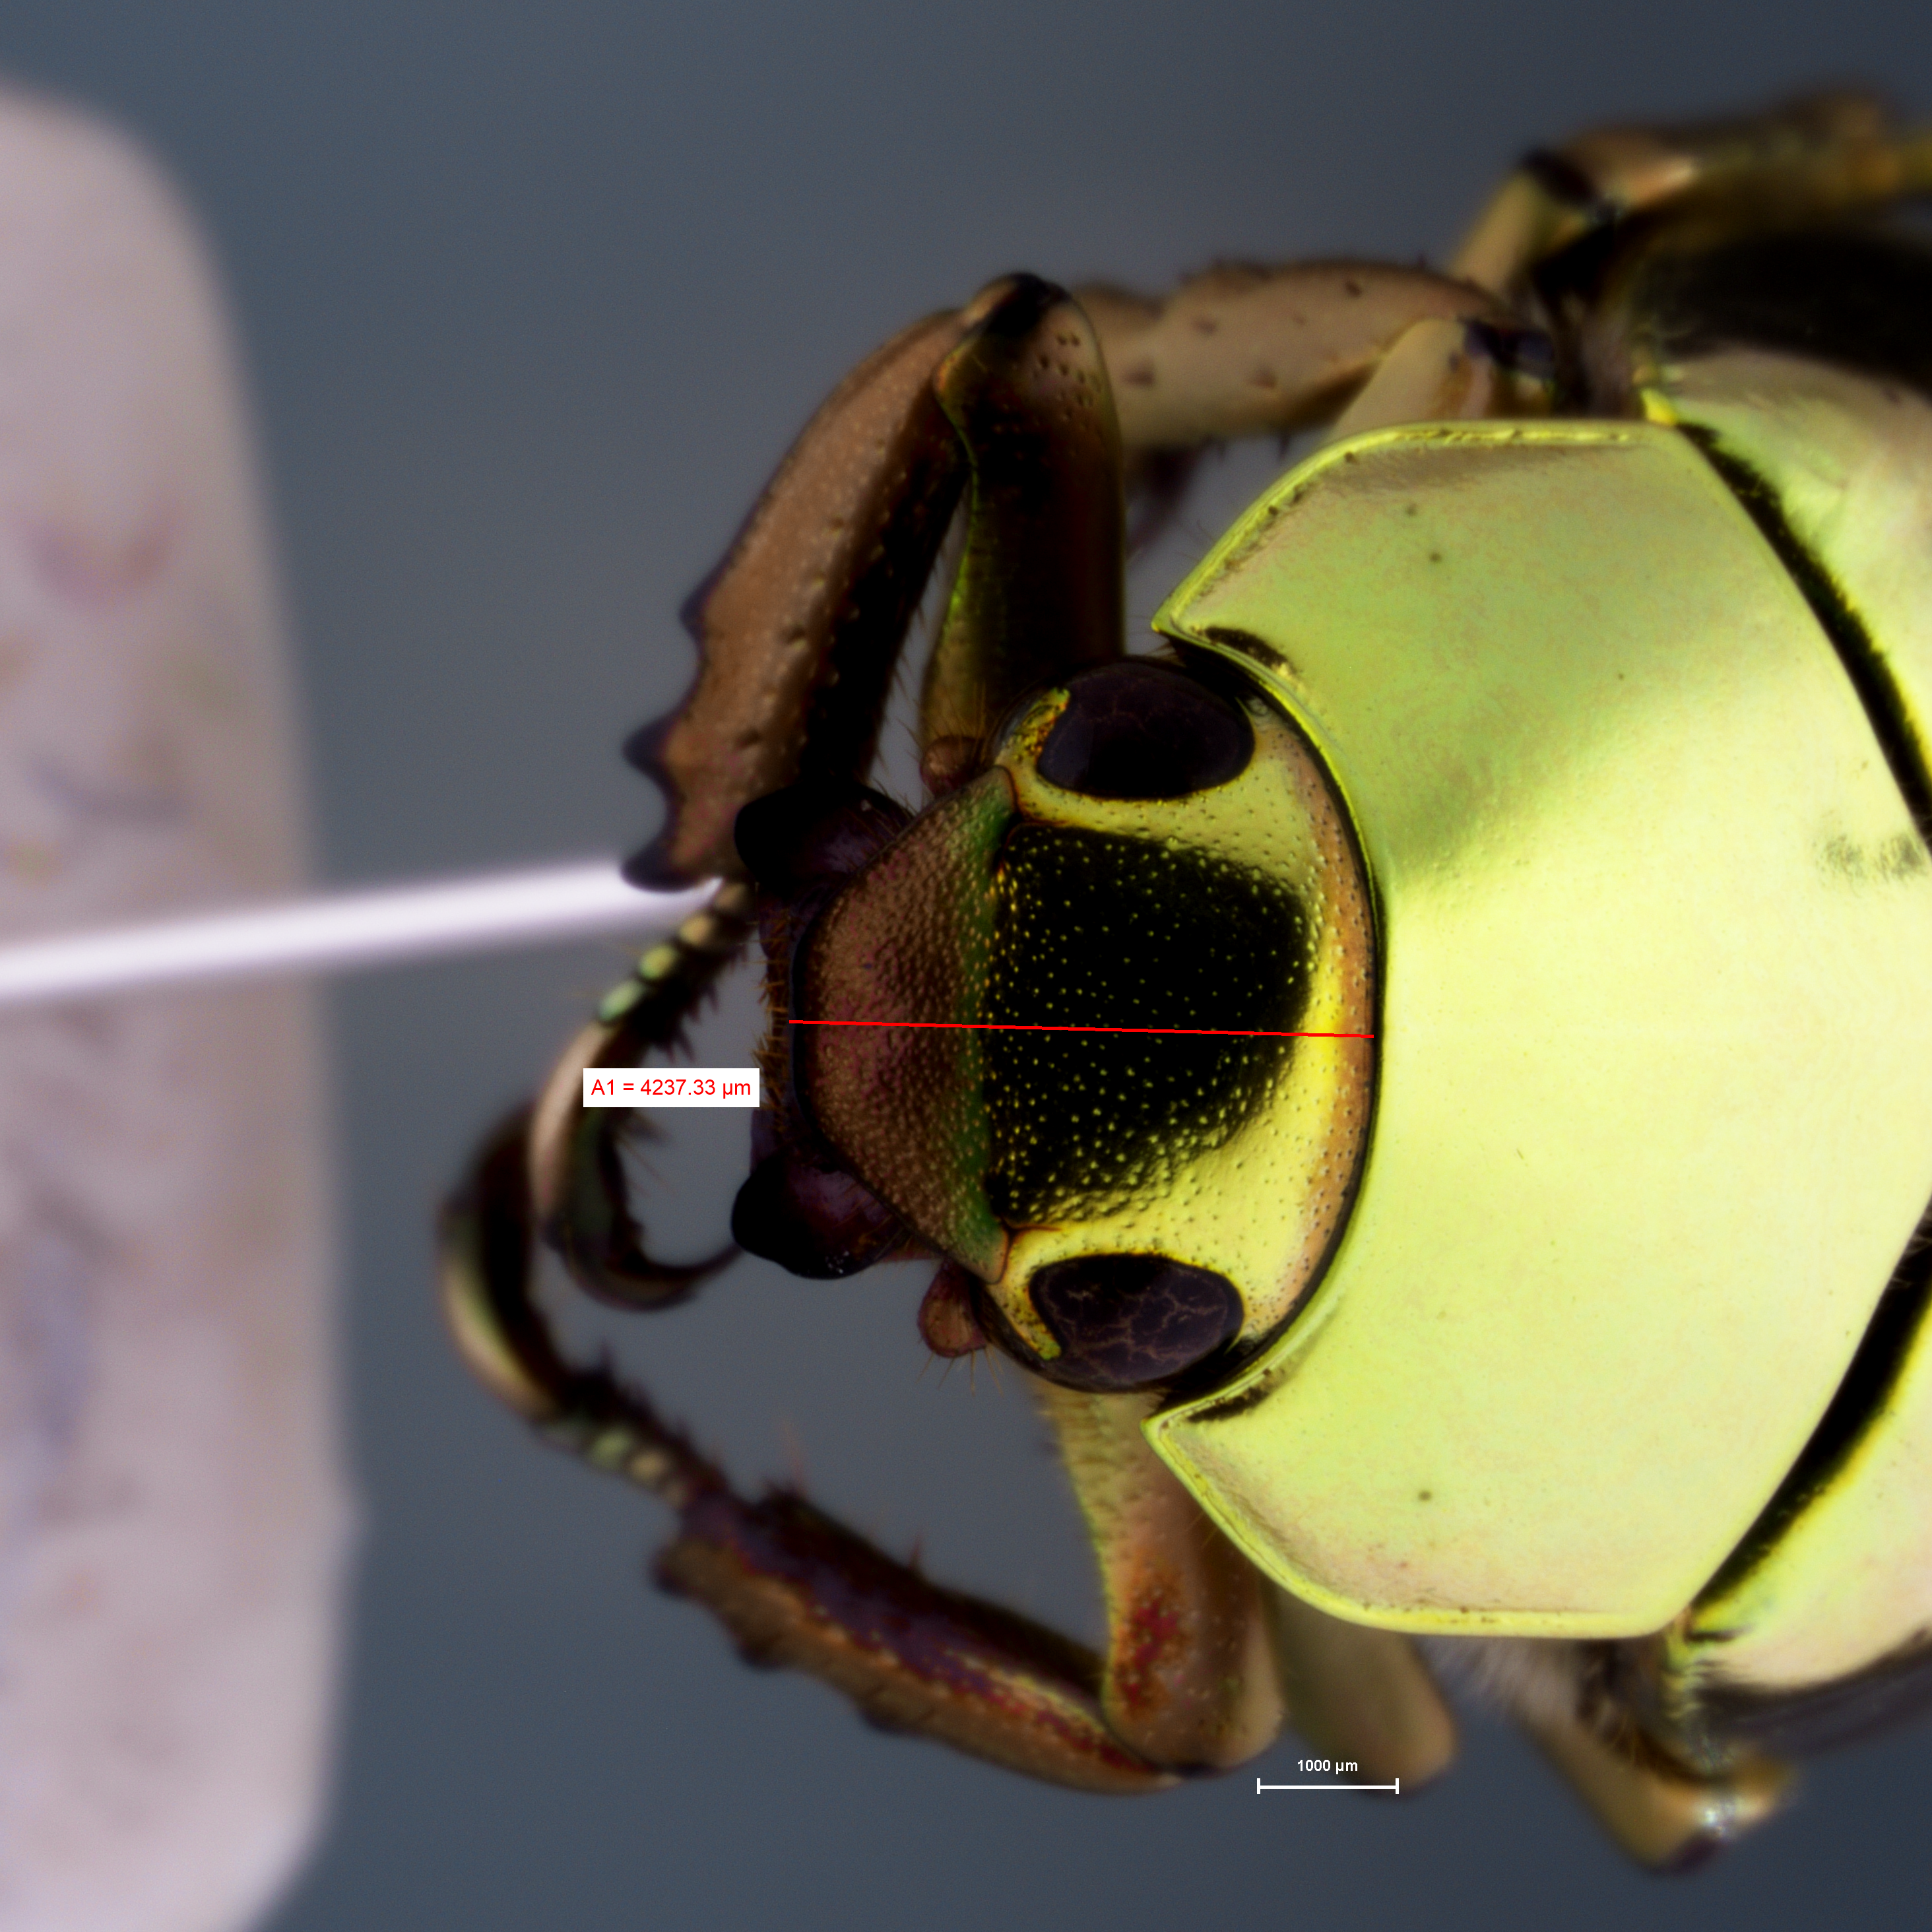
\includegraphics[width=0.5\linewidth]{images/protocol/Head_A1.png}
\caption{ Metric A1}
\end{figure}

\newpage
\subsection*{Metric: A2}

Horizontal length between the left and right sutures

\begin{figure}[H]
\centering
\includegraphics[width=0.7\linewidth]{images/boxplot/boxplot_A2.png}
\caption{  Boxplot and specimen distribution (superposed) for the metric  A2 by species}
\end{figure}

\noindent\textbf{Test Type:} Student's t-test \\
\noindent\textbf{Test Statistic:} -2.168 \\
\noindent\textbf{P-value:} 0.039 \\
\noindent\textbf{Interpretation:} significant difference

\begin{figure}[H]
\centering
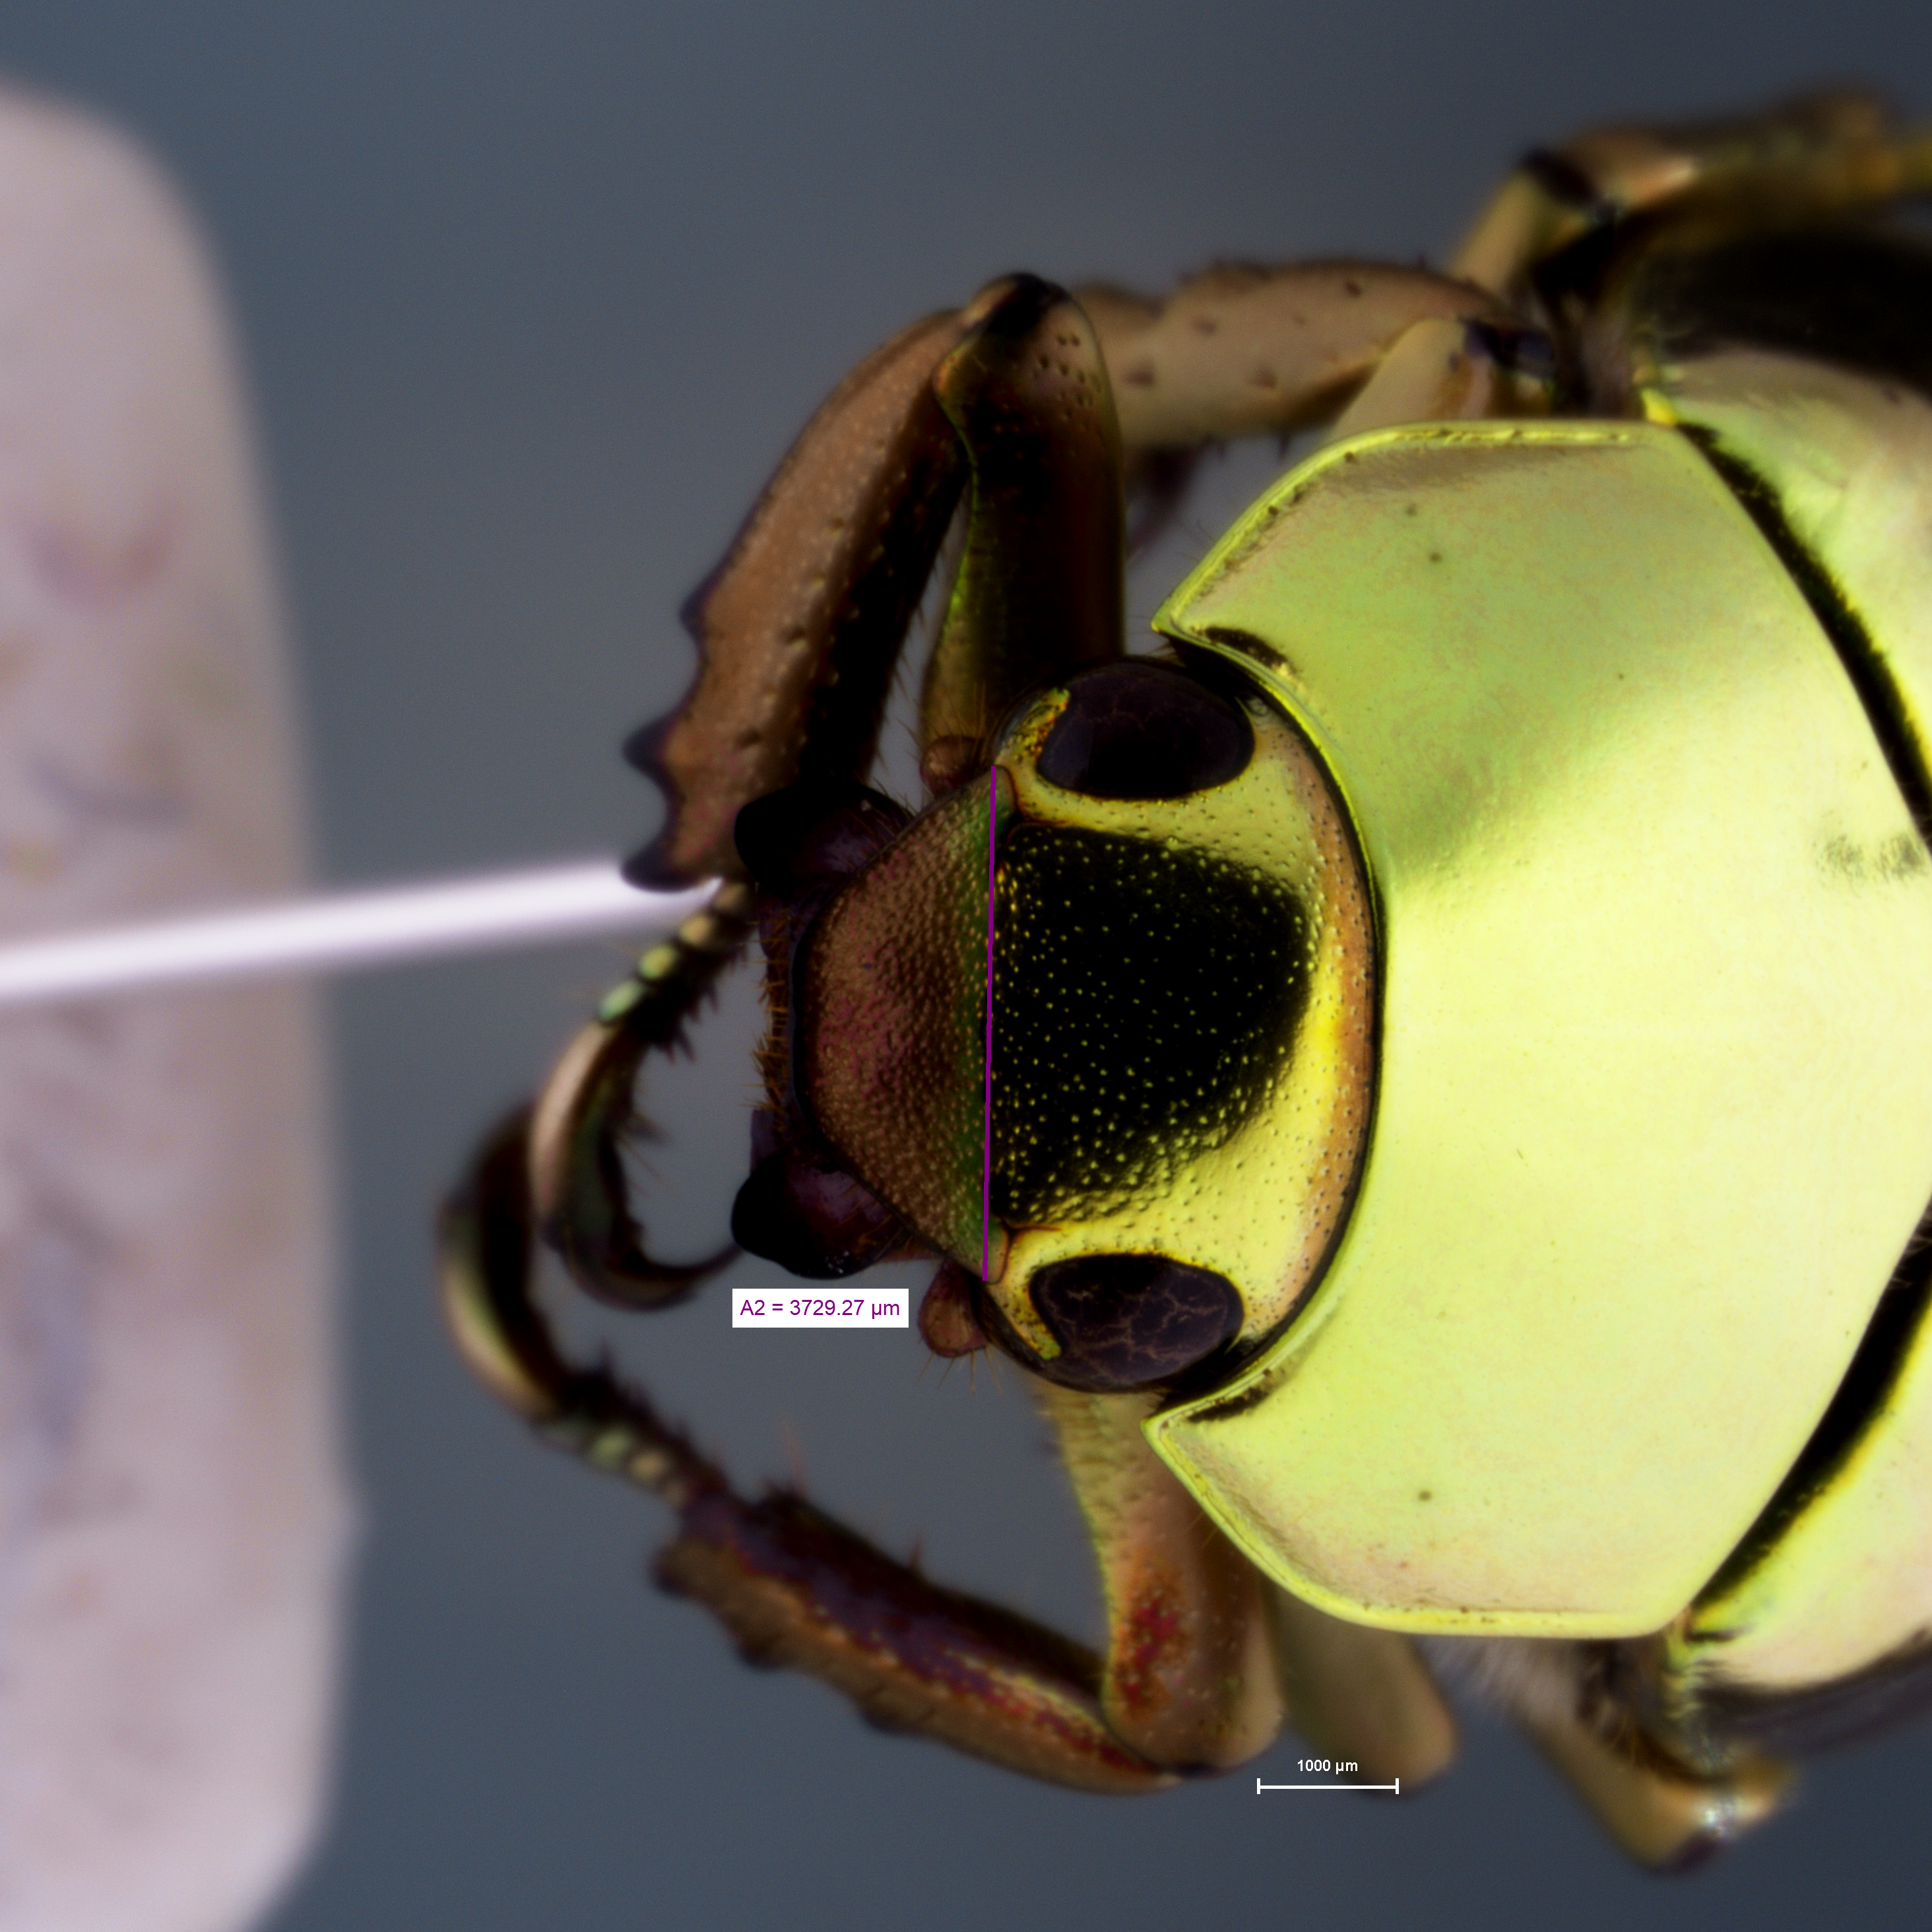
\includegraphics[width=0.5\linewidth]{images/protocol/Head_A2.png}
\caption{ Metric A2}
\end{figure}

\newpage
\subsection*{Metric: A3}

Horizontal length between the left and right eye’s canthus

\begin{figure}[H]
\centering
\includegraphics[width=0.7\linewidth]{images/boxplot/boxplot_A3.png}
\caption{  Boxplot and specimen distribution (superposed) for the metric  A3 by species}
\end{figure}

\noindent\textbf{Test Type:} Student's t-test \\
\noindent\textbf{Test Statistic:} -3.297 \\
\noindent\textbf{P-value:} 0.003 \\
\noindent\textbf{Interpretation:} significant difference

\begin{figure}[H]
\centering
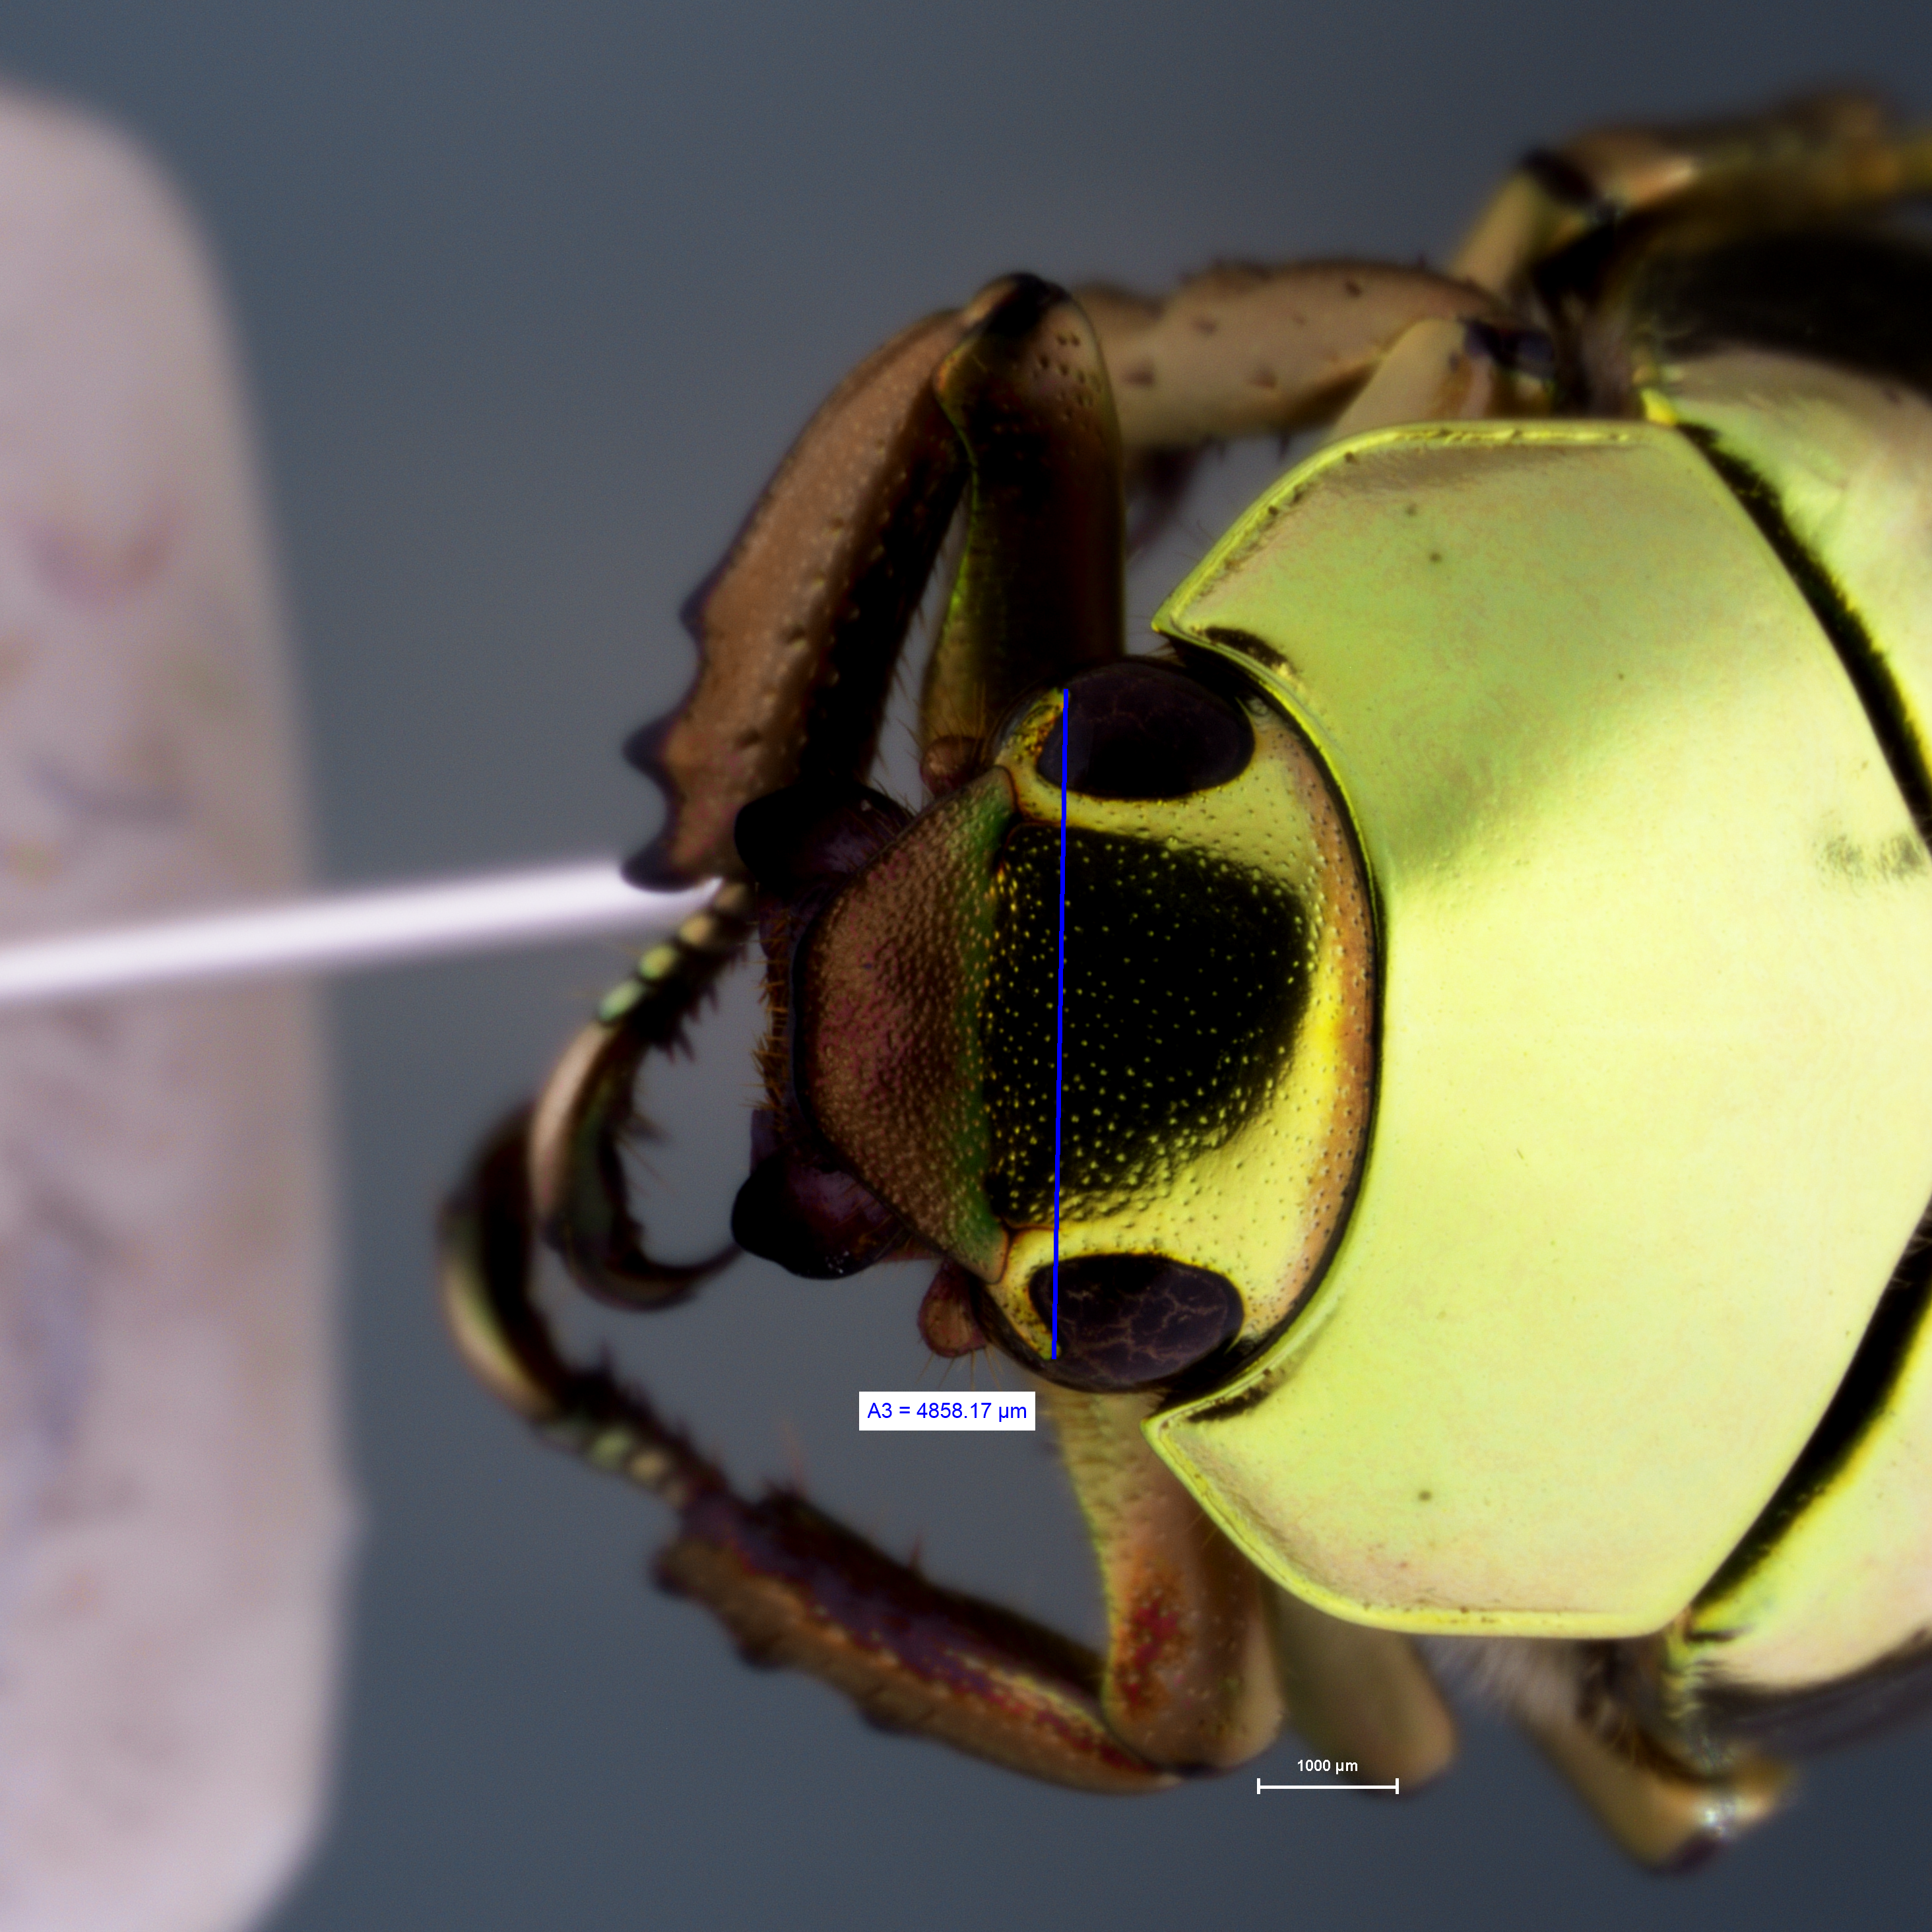
\includegraphics[width=0.5\linewidth]{images/protocol/Head_A3.png}
\caption{ Metric A3}
\end{figure}

\newpage
\subsection*{Metric: A4}

Vertical ortogonal length of the clipeus measured from the front down to A2 line

\begin{figure}[H]
\centering
\includegraphics[width=0.7\linewidth]{images/boxplot/boxplot_A4.png}
\caption{  Boxplot and specimen distribution (superposed) for the metric  A4 by species}
\end{figure}

\noindent\textbf{Test Type:} Mann-Whitney U test \\
\noindent\textbf{Test Statistic:} 46.000 \\
\noindent\textbf{P-value:} 0.232 \\
\noindent\textbf{Interpretation:} no significant difference

\begin{figure}[H]
\centering
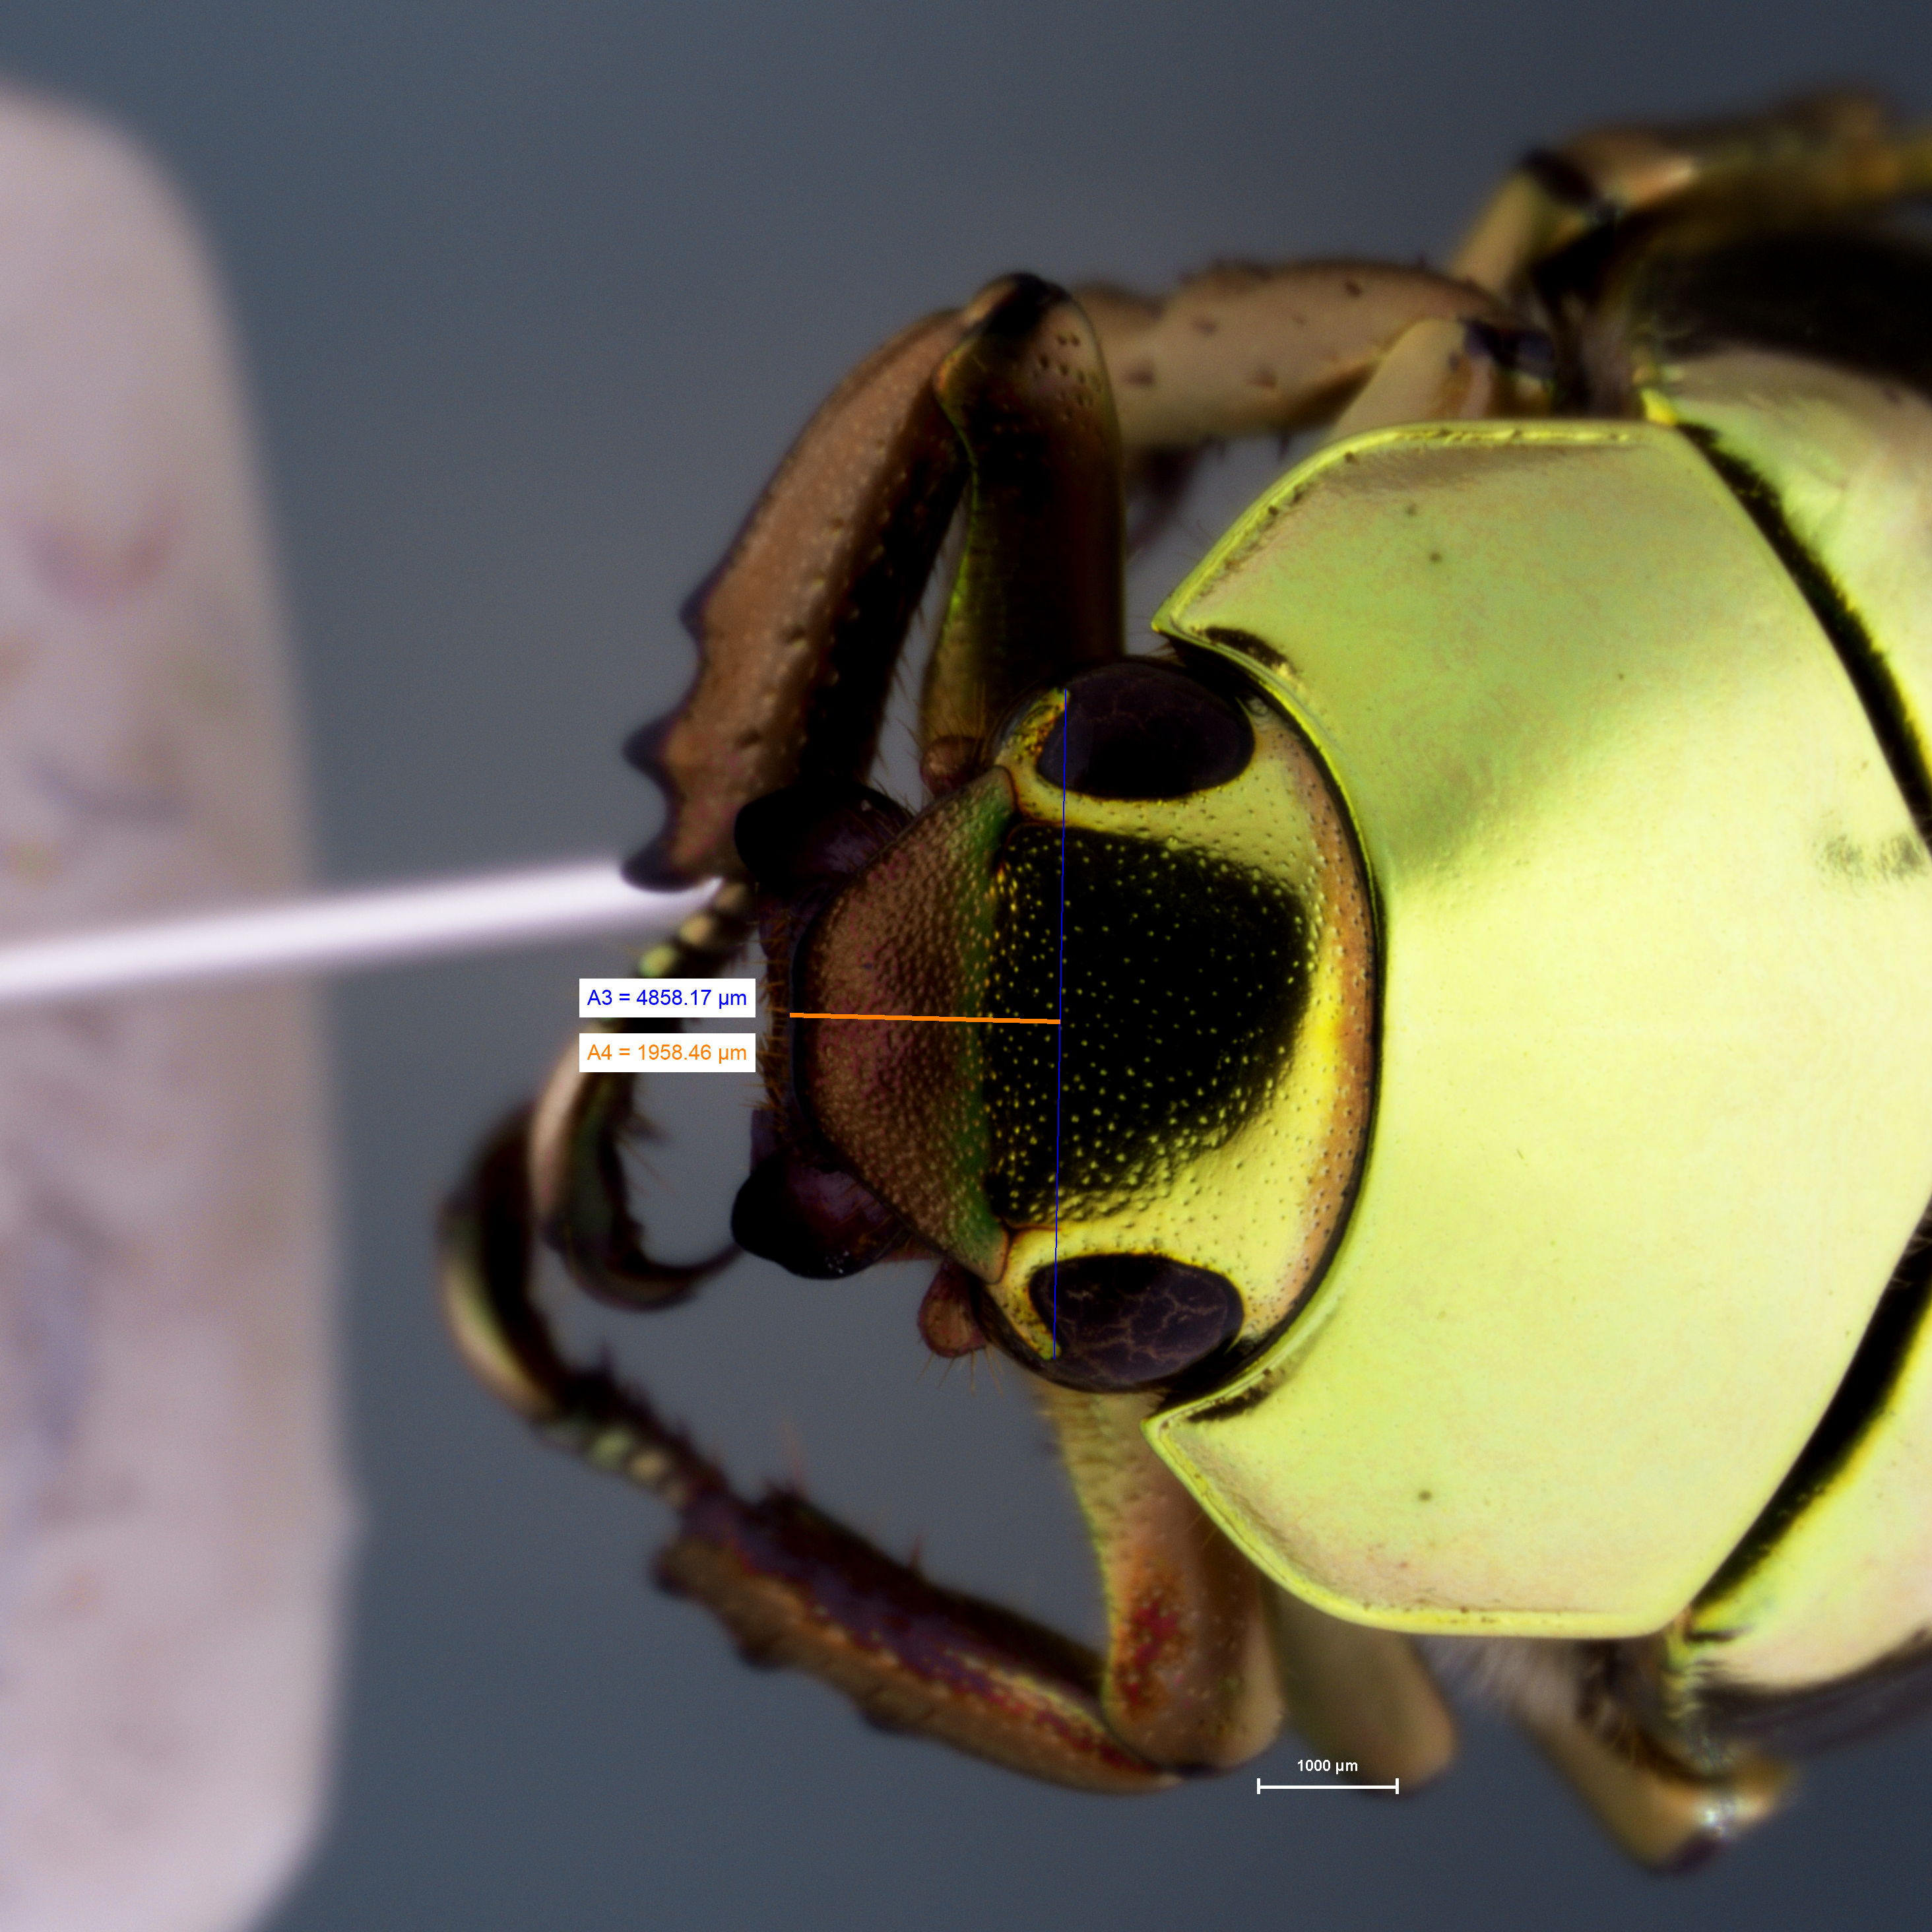
\includegraphics[width=0.5\linewidth]{images/protocol/Head_A4.png}
\caption{ Metric A4}
\end{figure}

\newpage
\subsection*{Metric: A5}

Perpendicular vertical length of the clypeus, measured from its front edge to the $A2$ line, representing the clypeus height.

\begin{figure}[H]
\centering
\includegraphics[width=0.7\linewidth]{images/boxplot/boxplot_A5.png}
\caption{  Boxplot and specimen distribution (superposed) for the metric  A5 by species}
\end{figure}

\noindent\textbf{Test Type:} Mann-Whitney U test \\
\noindent\textbf{Test Statistic:} 68.000 \\
\noindent\textbf{P-value:} 0.979 \\
\noindent\textbf{Interpretation:} no significant difference

\begin{figure}[H]
\centering
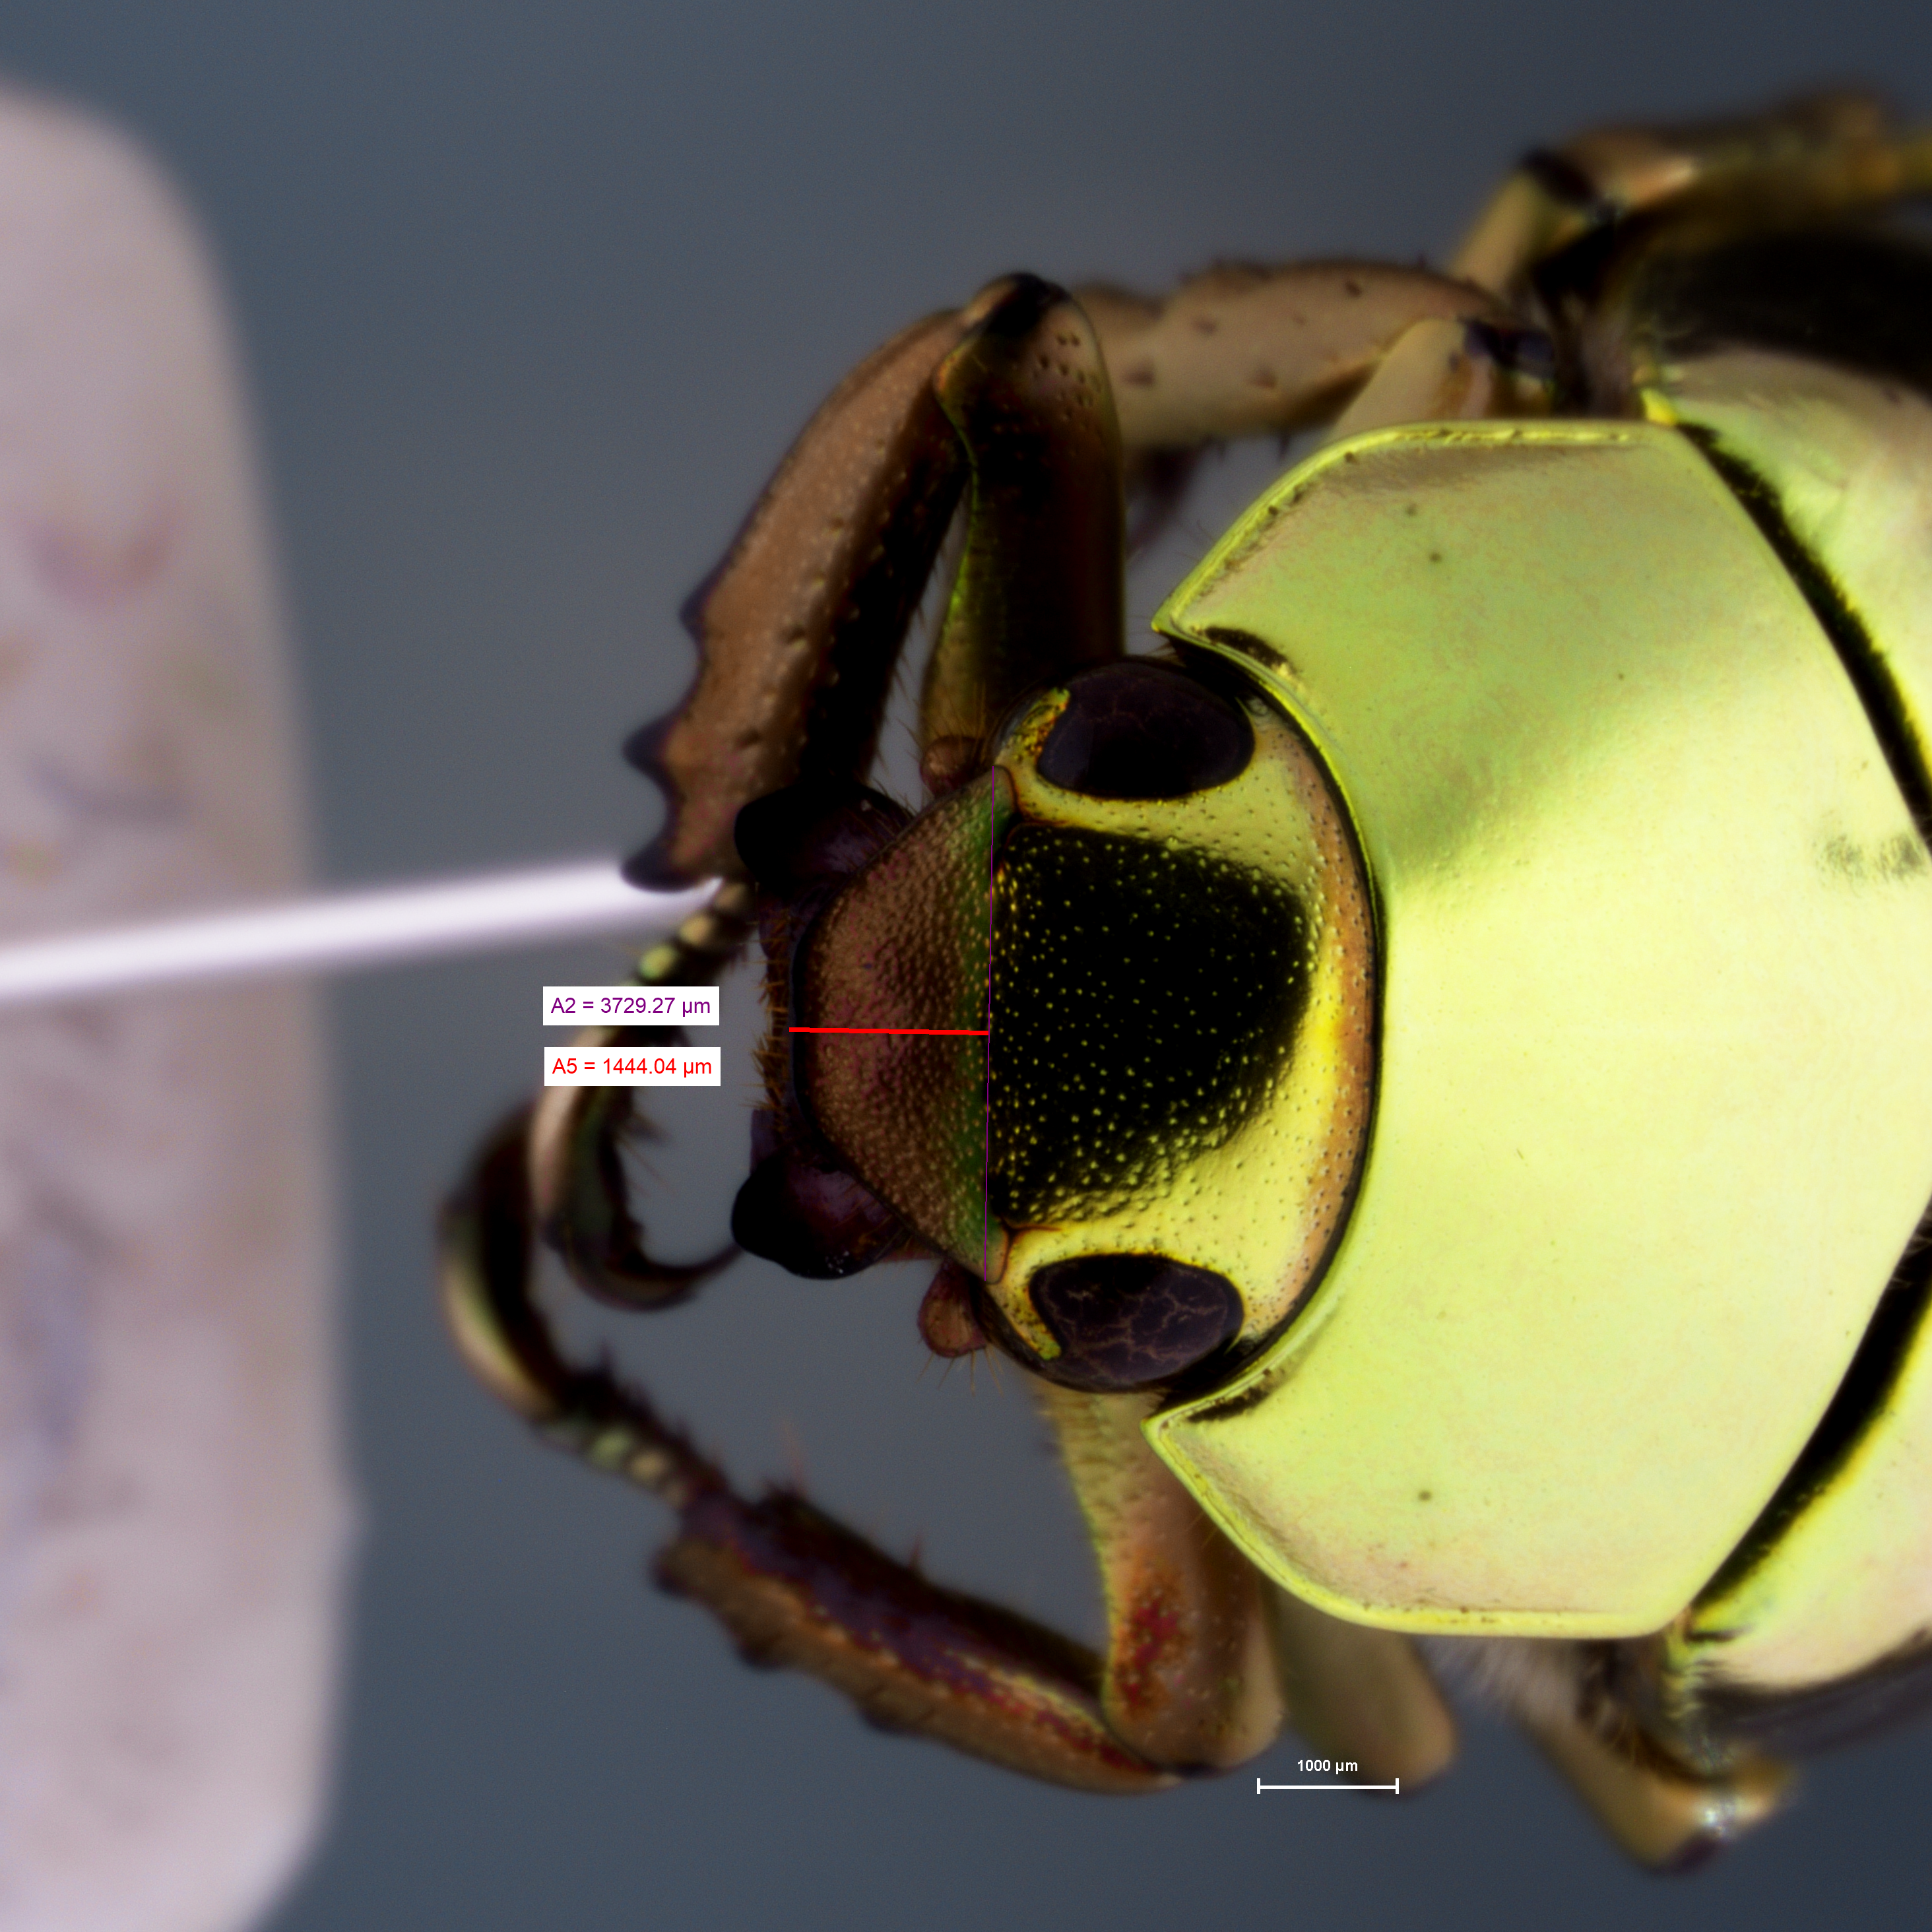
\includegraphics[width=0.5\linewidth]{images/protocol/Head_A5.png}
\caption{ Metric A5}
\end{figure}

\newpage
\subsection*{Metric: B1}

Horizontal length between the pronotum’s frontal angles

\begin{figure}[H]
\centering
\includegraphics[width=0.7\linewidth]{images/boxplot/boxplot_B1.png}
\caption{  Boxplot and specimen distribution (superposed) for the metric  B1 by species}
\end{figure}

\noindent\textbf{Test Type:} Mann-Whitney U test \\
\noindent\textbf{Test Statistic:} 58.000 \\
\noindent\textbf{P-value:} 0.012 \\
\noindent\textbf{Interpretation:} significant difference

\begin{figure}[H]
\centering
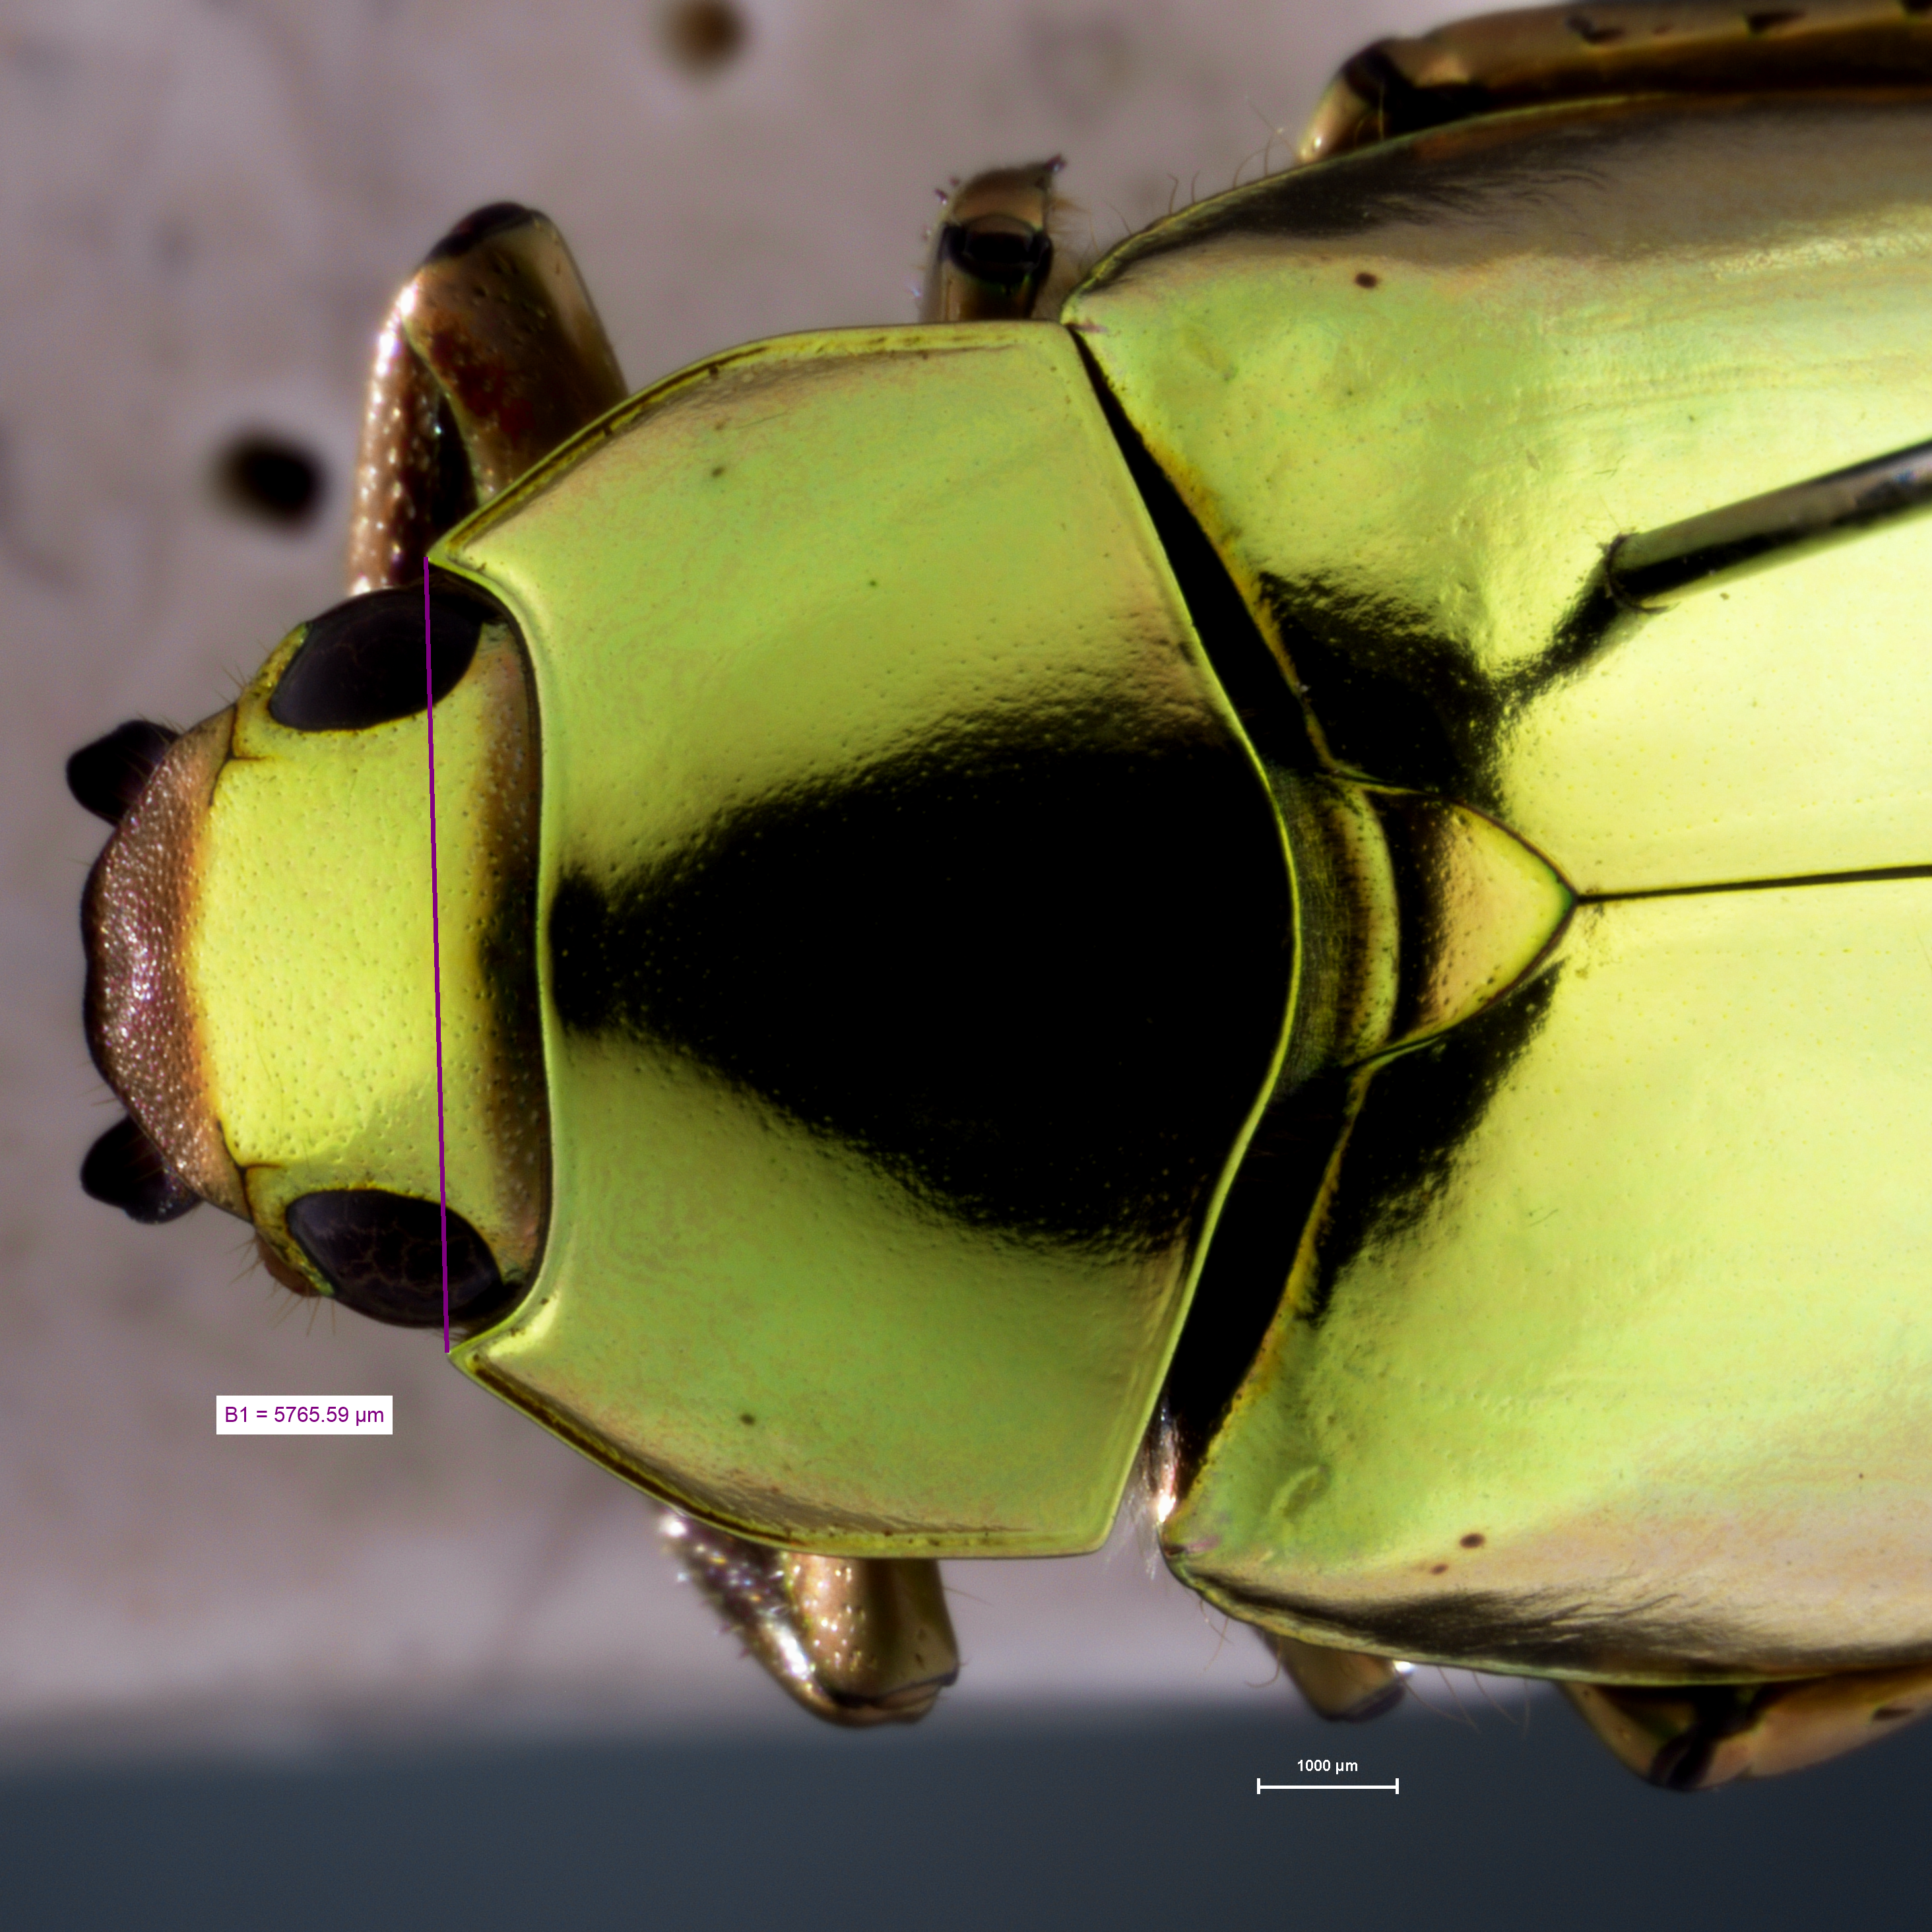
\includegraphics[width=0.5\linewidth]{images/protocol/Pronotum_B1.png}
\caption{ Metric B1}
\end{figure}

\newpage
\subsection*{Metric: B2}

Horizontal length between the pronotum’s middle angles

\begin{figure}[H]
\centering
\includegraphics[width=0.7\linewidth]{images/boxplot/boxplot_B2.png}
\caption{  Boxplot and specimen distribution (superposed) for the metric  B2 by species}
\end{figure}

\noindent\textbf{Test Type:} Student's t-test \\
\noindent\textbf{Test Statistic:} -2.710 \\
\noindent\textbf{P-value:} 0.011 \\
\noindent\textbf{Interpretation:} significant difference

\begin{figure}[H]
\centering
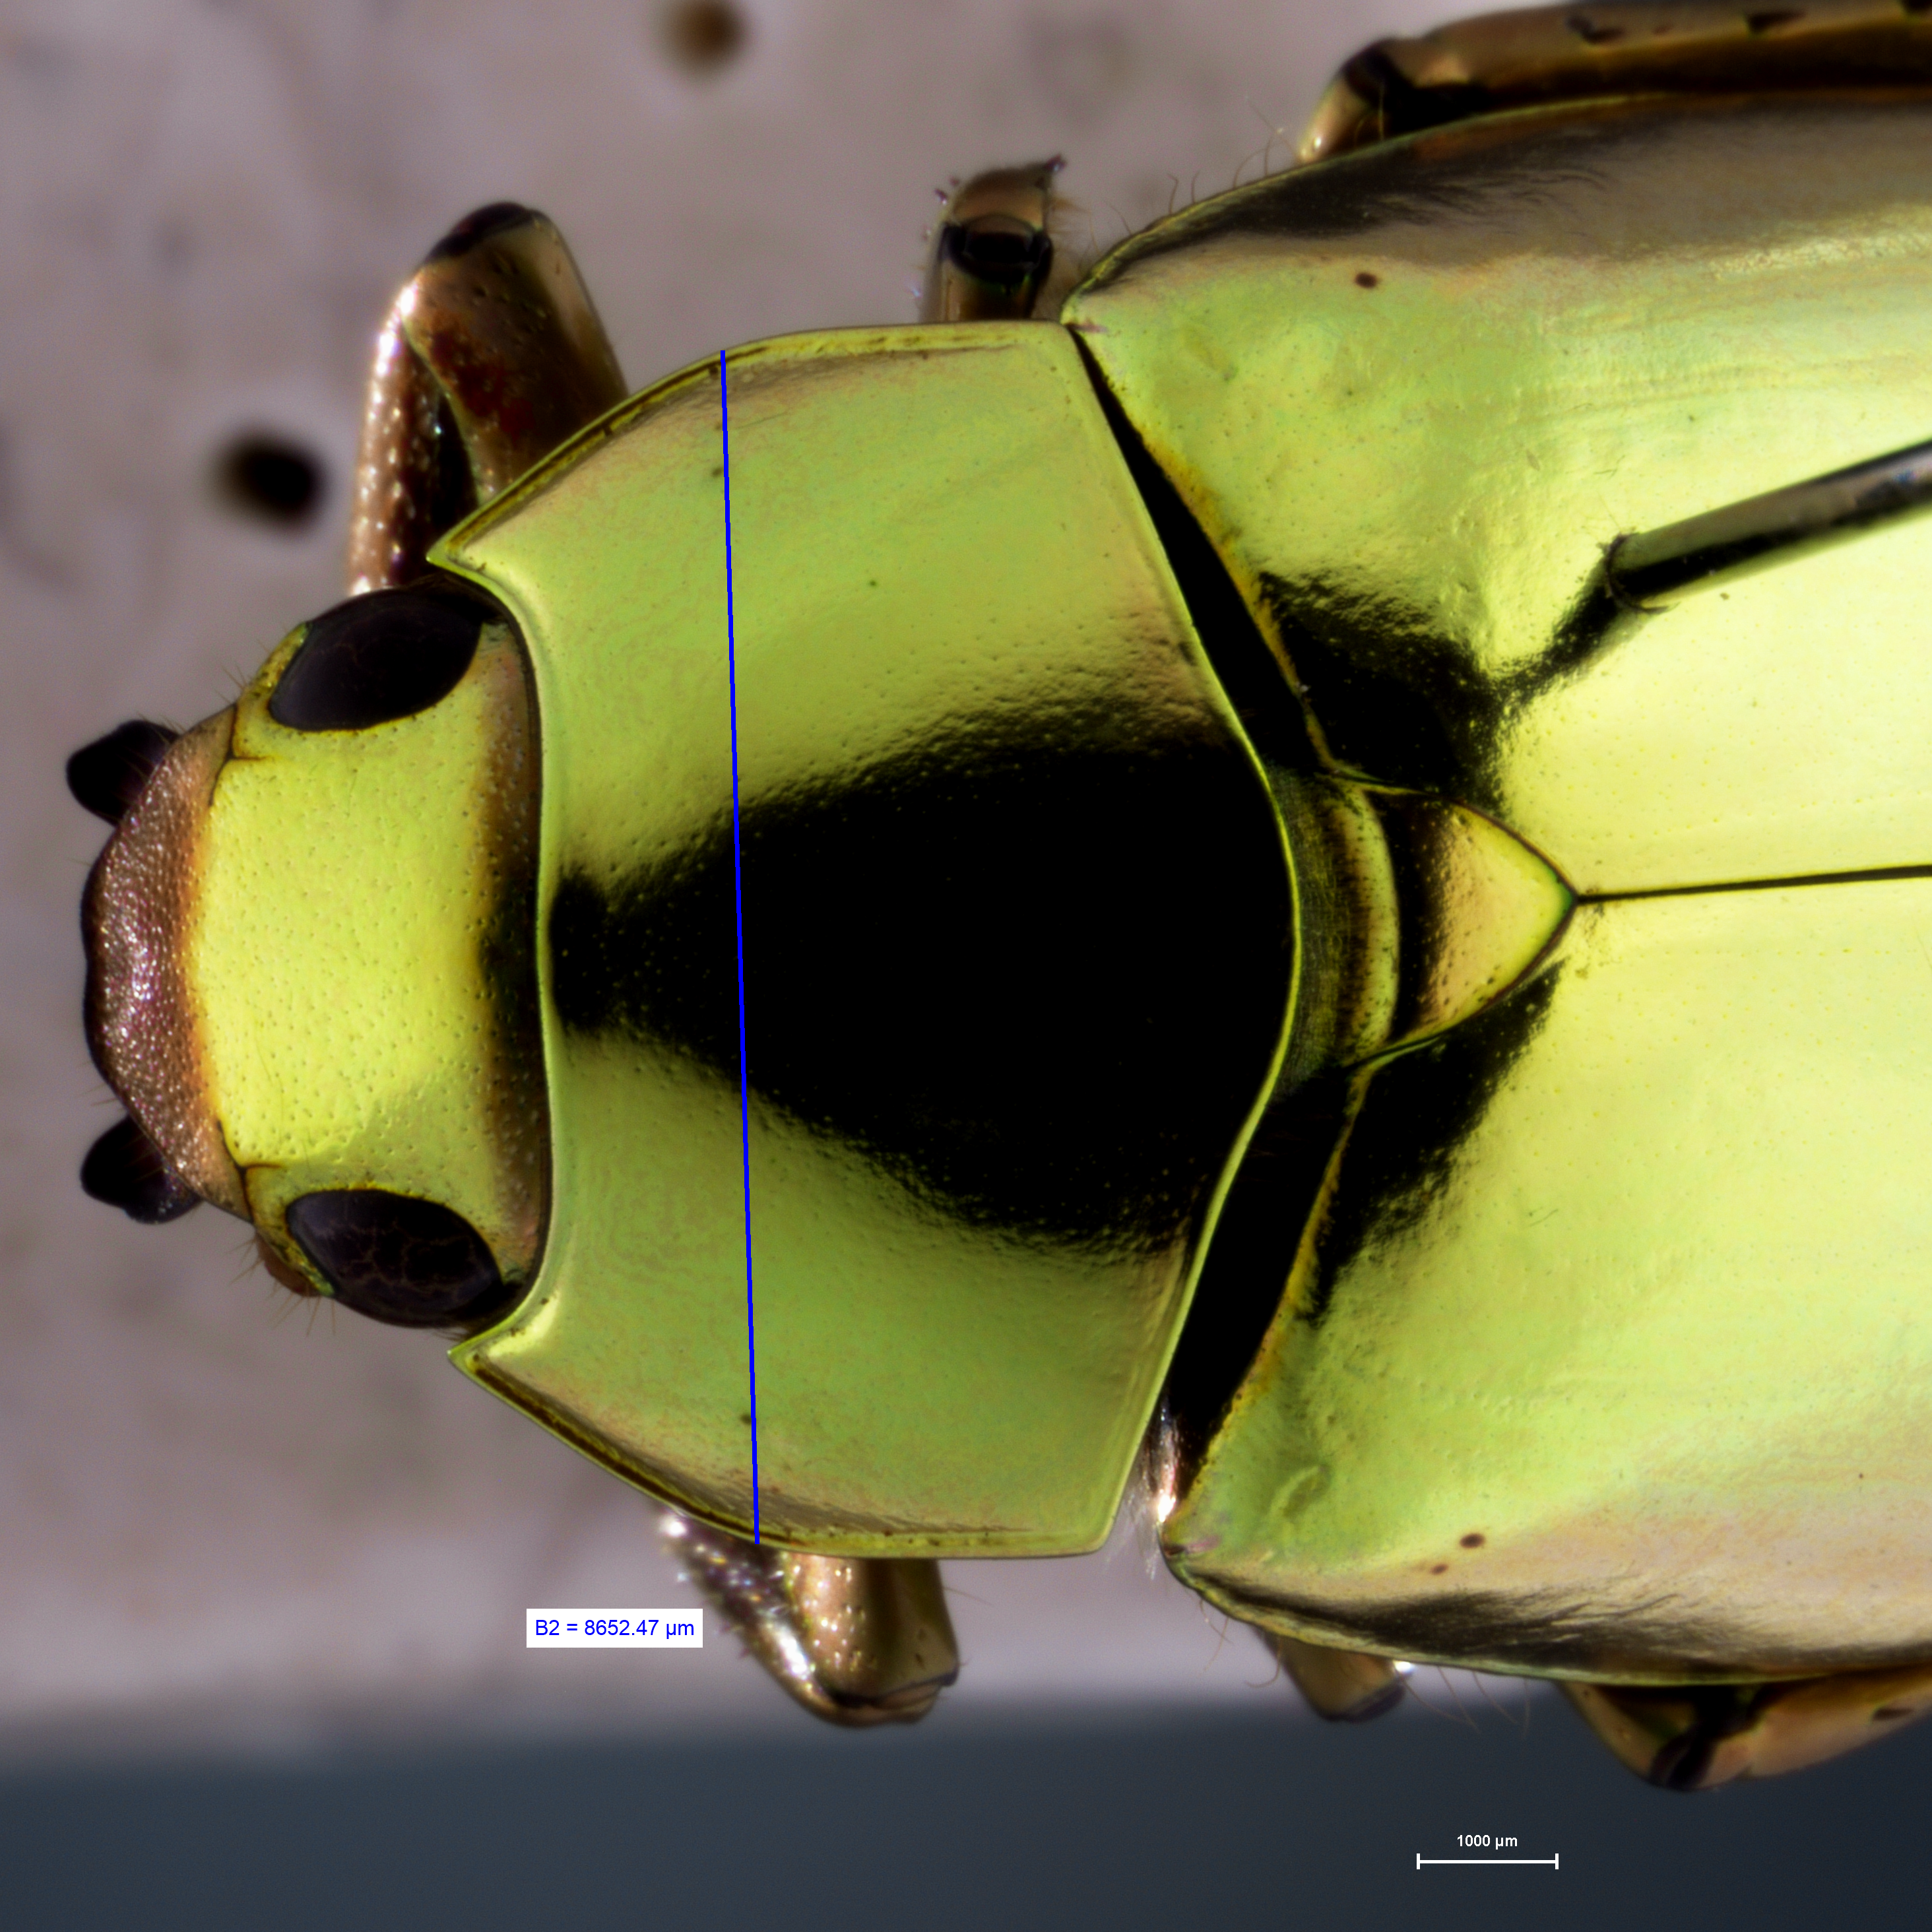
\includegraphics[width=0.5\linewidth]{images/protocol/Pronotum_B2.png}
\caption{ Metric B2}
\end{figure}

\newpage
\subsection*{Metric: B3}

Horizontal length between the pronotum’s hind angles

\begin{figure}[H]
\centering
\includegraphics[width=0.7\linewidth]{images/boxplot/boxplot_B3.png}
\caption{  Boxplot and specimen distribution (superposed) for the metric  B3 by species}
\end{figure}

\noindent\textbf{Test Type:} Student's t-test \\
\noindent\textbf{Test Statistic:} -1.697 \\
\noindent\textbf{P-value:} 0.099 \\
\noindent\textbf{Interpretation:} no significant difference

\begin{figure}[H]
\centering
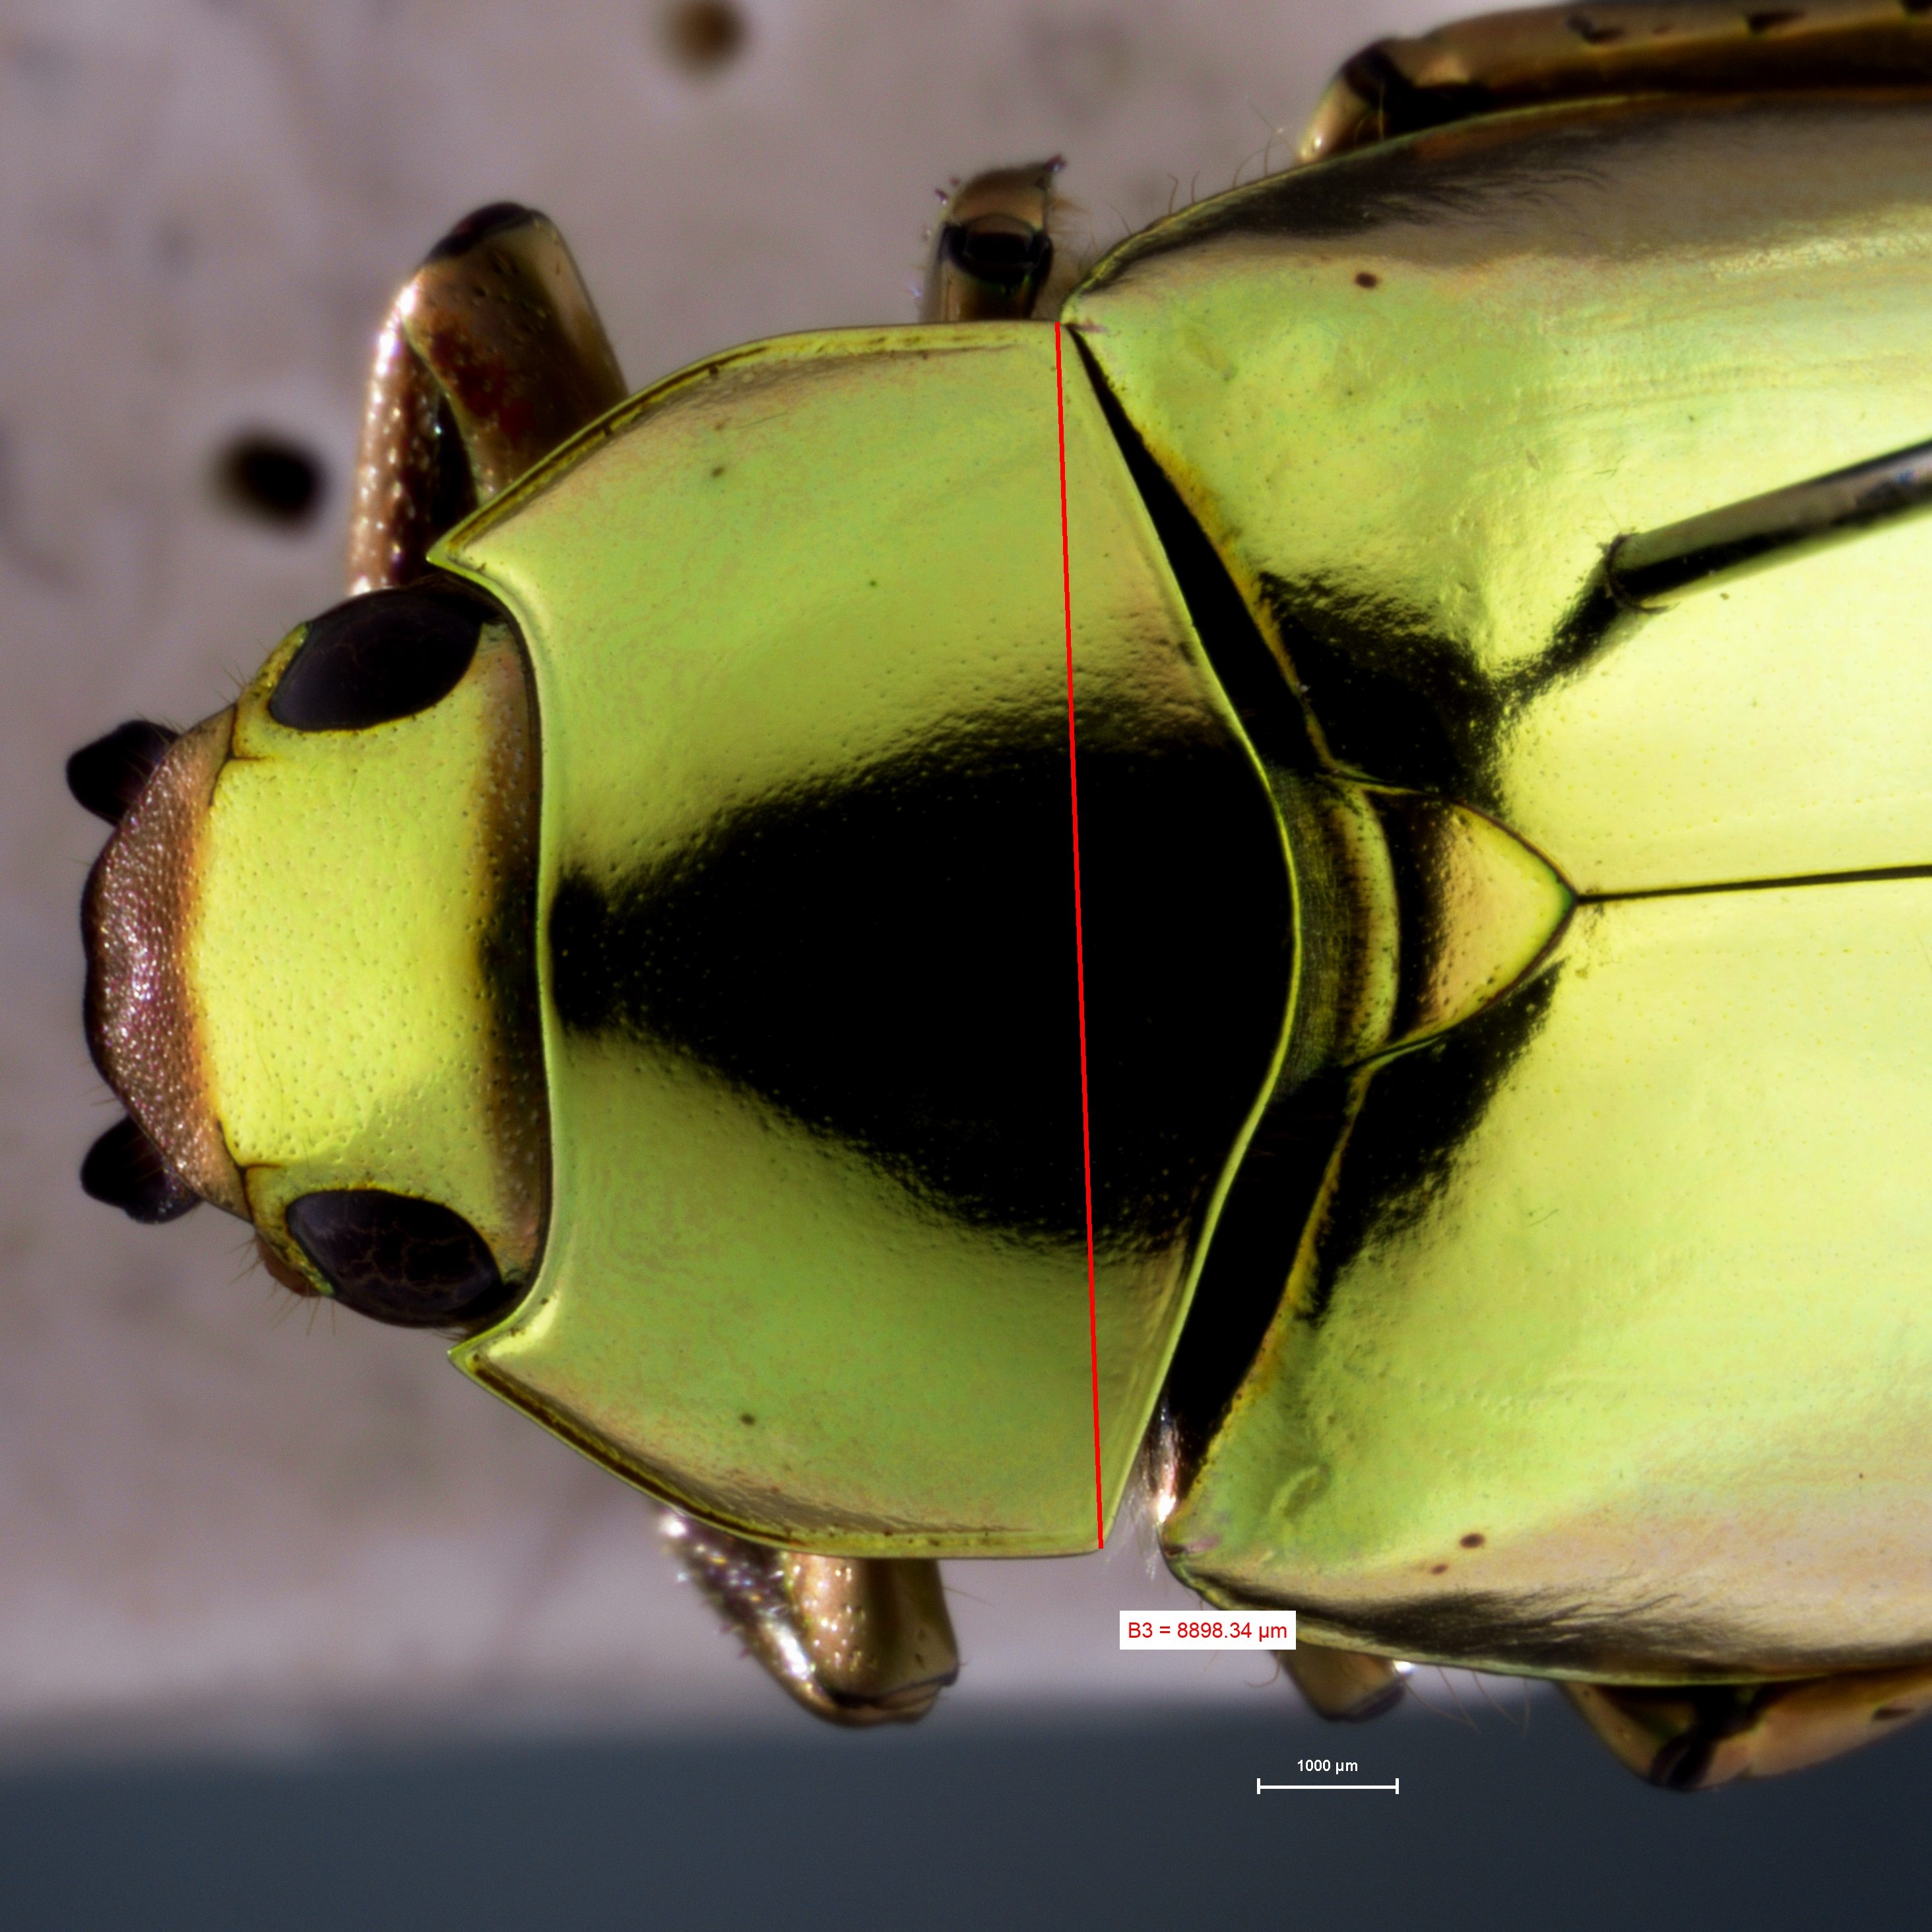
\includegraphics[width=0.5\linewidth]{images/protocol/Pronotum_B3.png}
\caption{ Metric B3}
\end{figure}

\newpage
\subsection*{Metric: B4}

Vertical length of the pronotum’s measured from the middle point of its front down to the middlepoint of its rear

\begin{figure}[H]
\centering
\includegraphics[width=0.7\linewidth]{images/boxplot/boxplot_B4.png}
\caption{  Boxplot and specimen distribution (superposed) for the metric  B4 by species}
\end{figure}

\noindent\textbf{Test Type:} Student's t-test \\
\noindent\textbf{Test Statistic:} -1.155 \\
\noindent\textbf{P-value:} 0.257 \\
\noindent\textbf{Interpretation:} no significant difference

\begin{figure}[H]
\centering
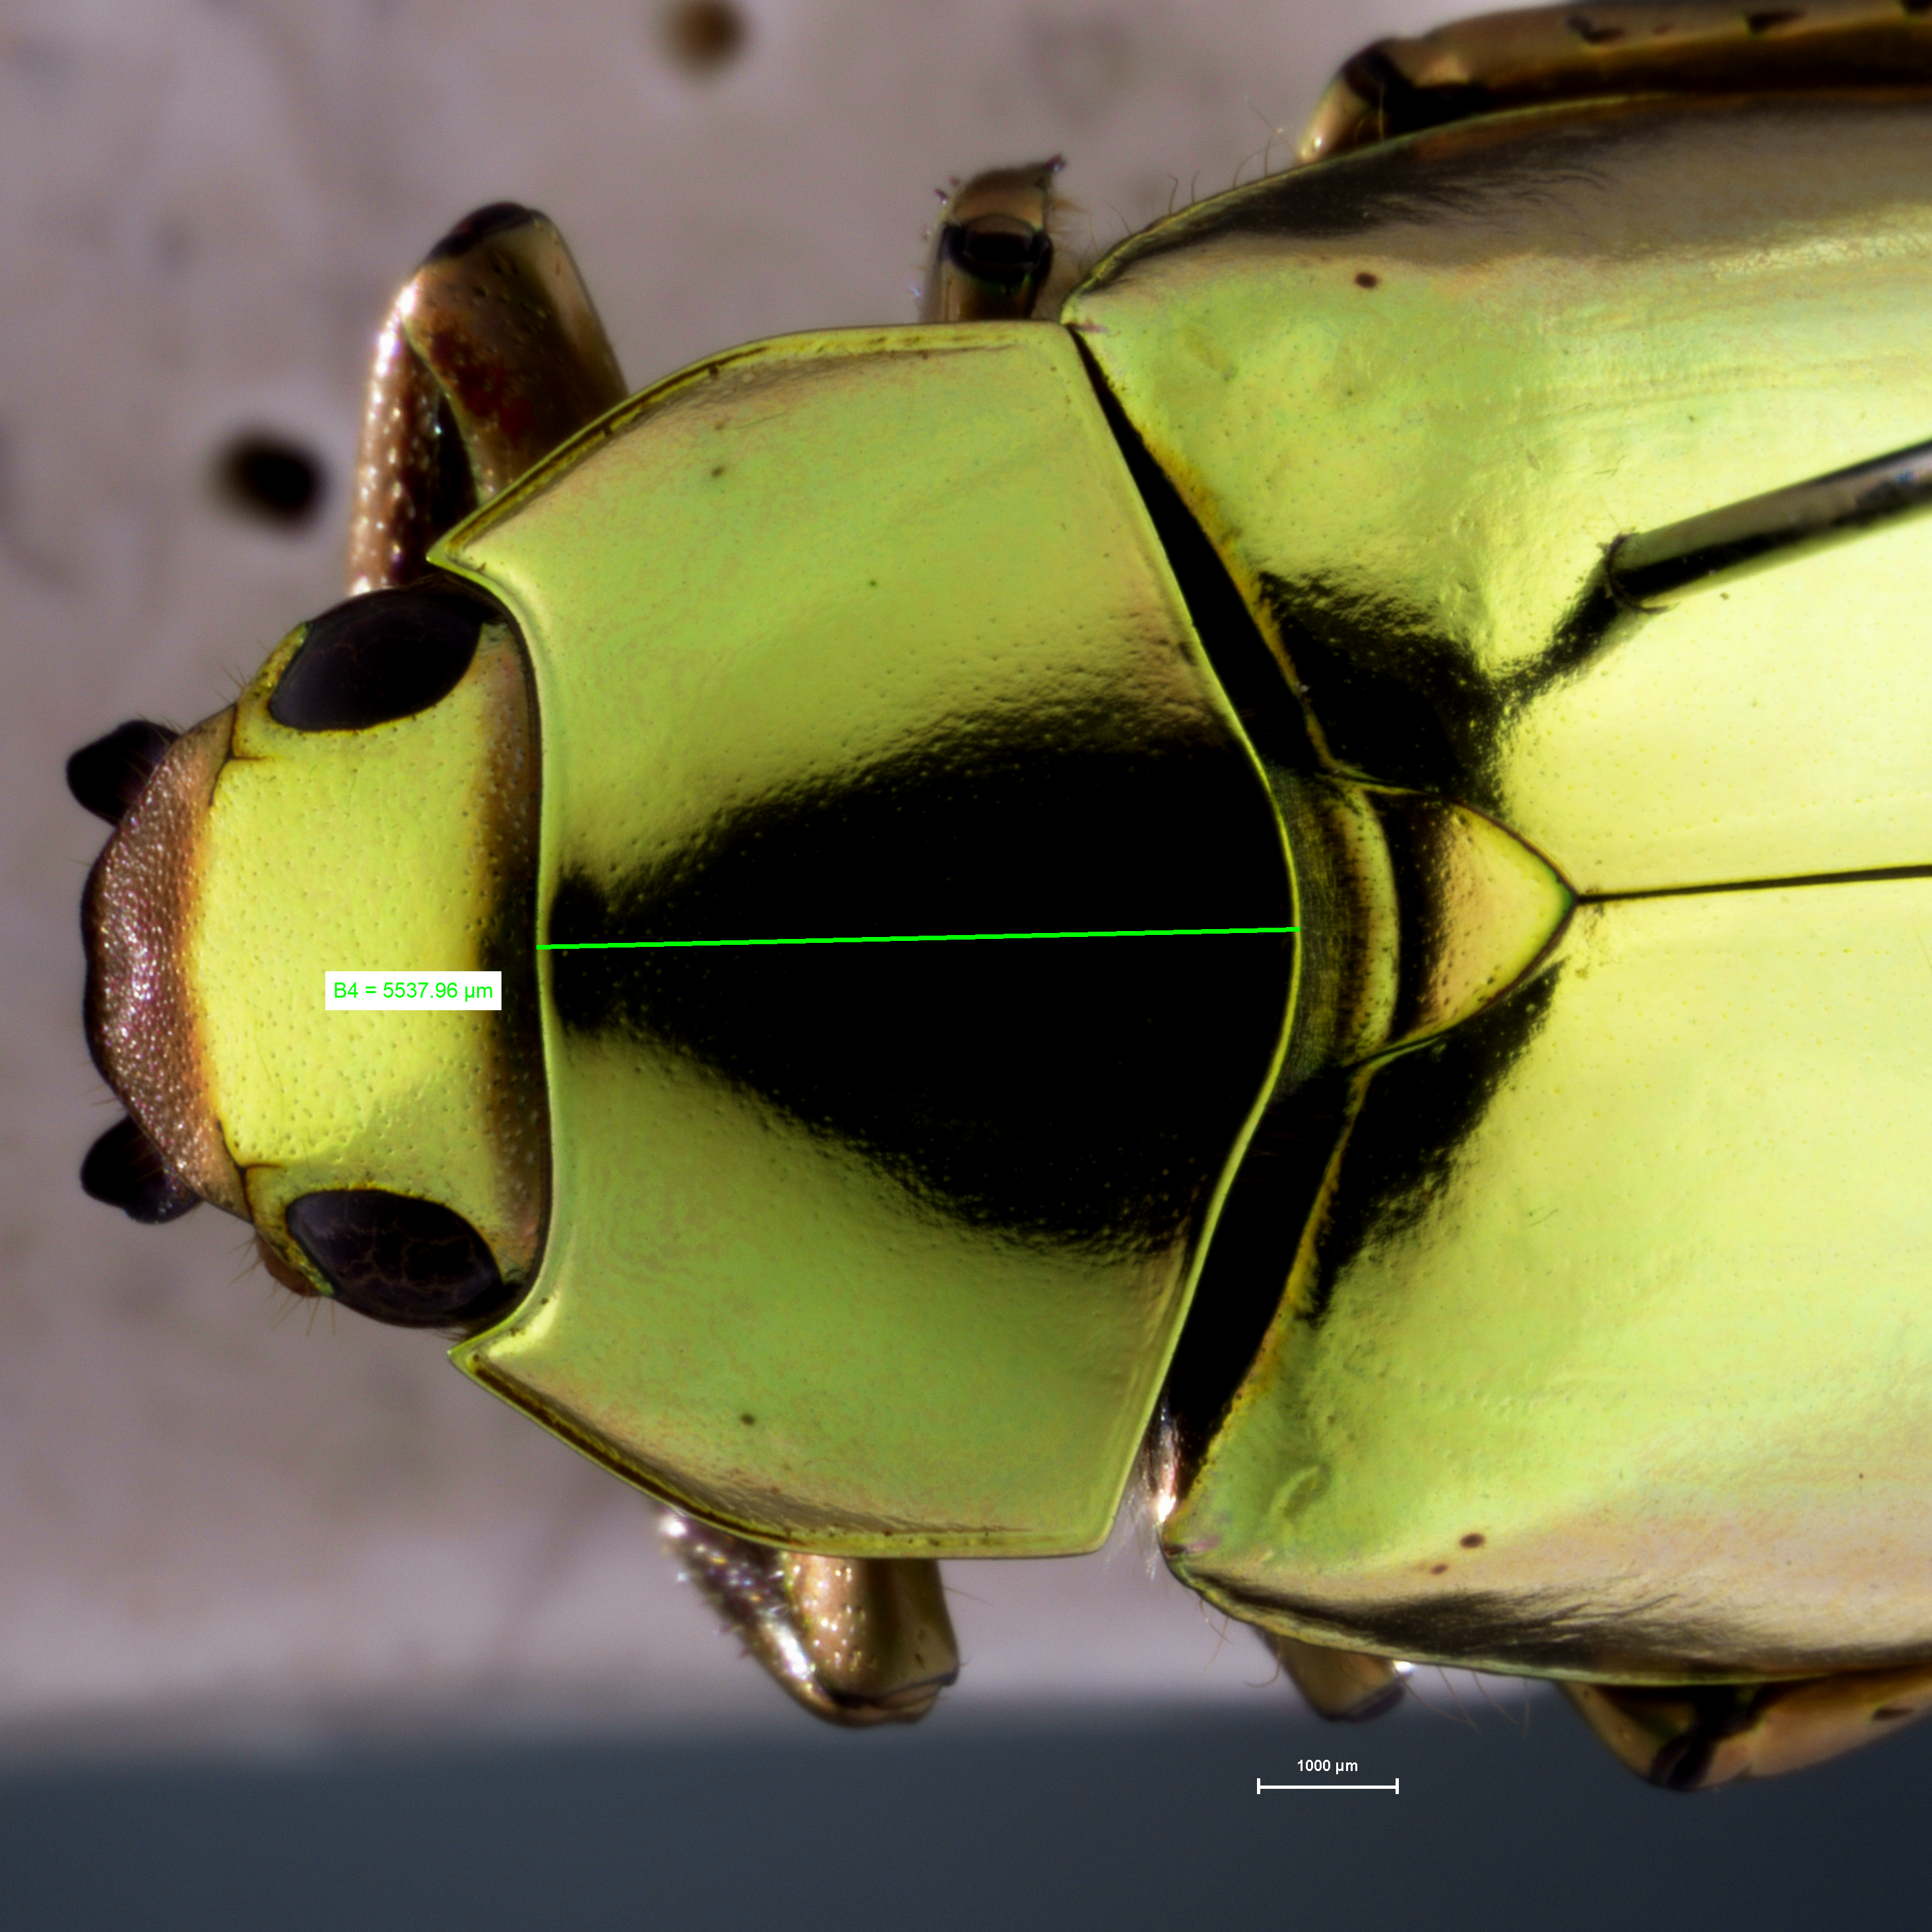
\includegraphics[width=0.5\linewidth]{images/protocol/Pronotum_B4.png}
\caption{ Metric B4}
\end{figure}

\newpage
\subsection*{Metric: B5}

Angle of its side measured between the tangent lines to its straightest sections in the front and back, as seen from the top 

\begin{figure}[H]
\centering
\includegraphics[width=0.7\linewidth]{images/boxplot/boxplot_B5.png}
\caption{  Boxplot and specimen distribution (superposed) for the metric  B5 by species}
\end{figure}

\noindent\textbf{Test Type:} Mann-Whitney U test \\
\noindent\textbf{Test Statistic:} 170.000 \\
\noindent\textbf{P-value:} 0.113 \\
\noindent\textbf{Interpretation:} no significant difference

\begin{figure}[H]
\centering
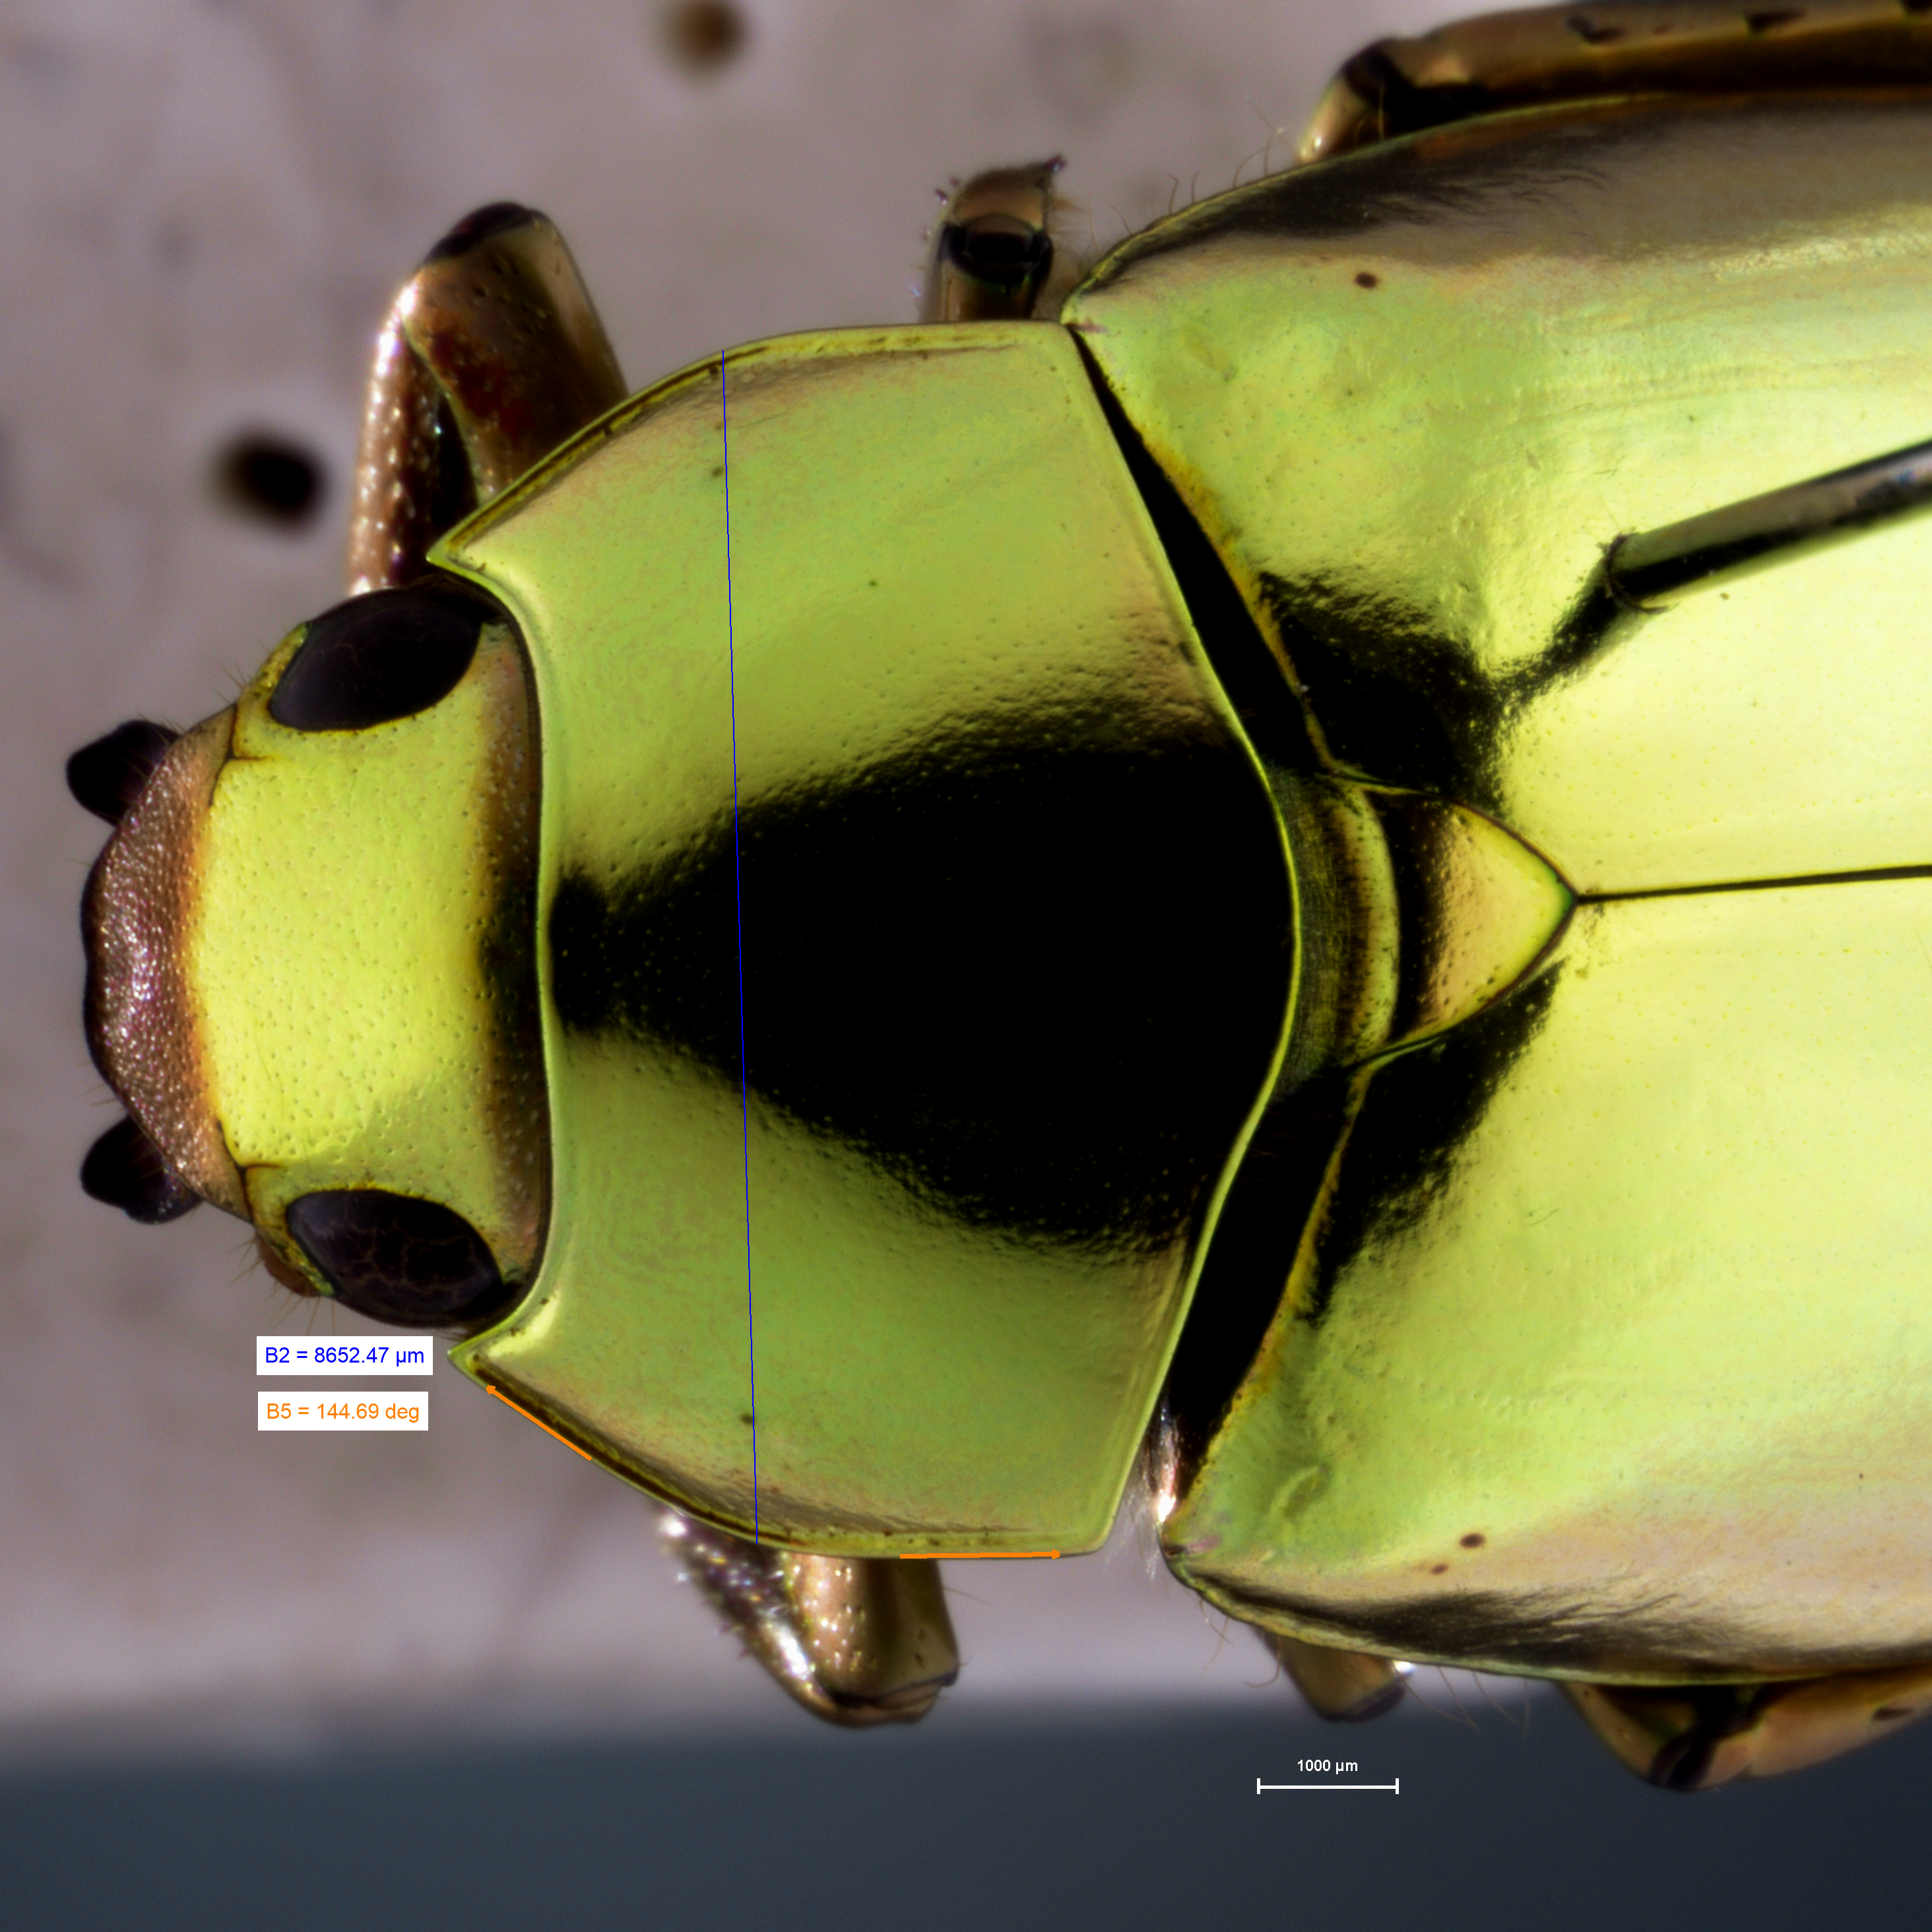
\includegraphics[width=0.5\linewidth]{images/protocol/Pronotum_B5.png}
\caption{ Metric B5}
\end{figure}

\newpage
\subsection*{Metric: C1}

Angle of its side measured between the tangent lines to its straightest sections in the front and back as seen by the side

\begin{figure}[H]
\centering
\includegraphics[width=0.7\linewidth]{images/boxplot/boxplot_C1.png}
\caption{  Boxplot and specimen distribution (superposed) for the metric  C1 by species}
\end{figure}

\noindent\textbf{Test Type:} Student's t-test \\
\noindent\textbf{Test Statistic:} 0.851 \\
\noindent\textbf{P-value:} 0.401 \\
\noindent\textbf{Interpretation:} no significant difference

\begin{figure}[H]
\centering
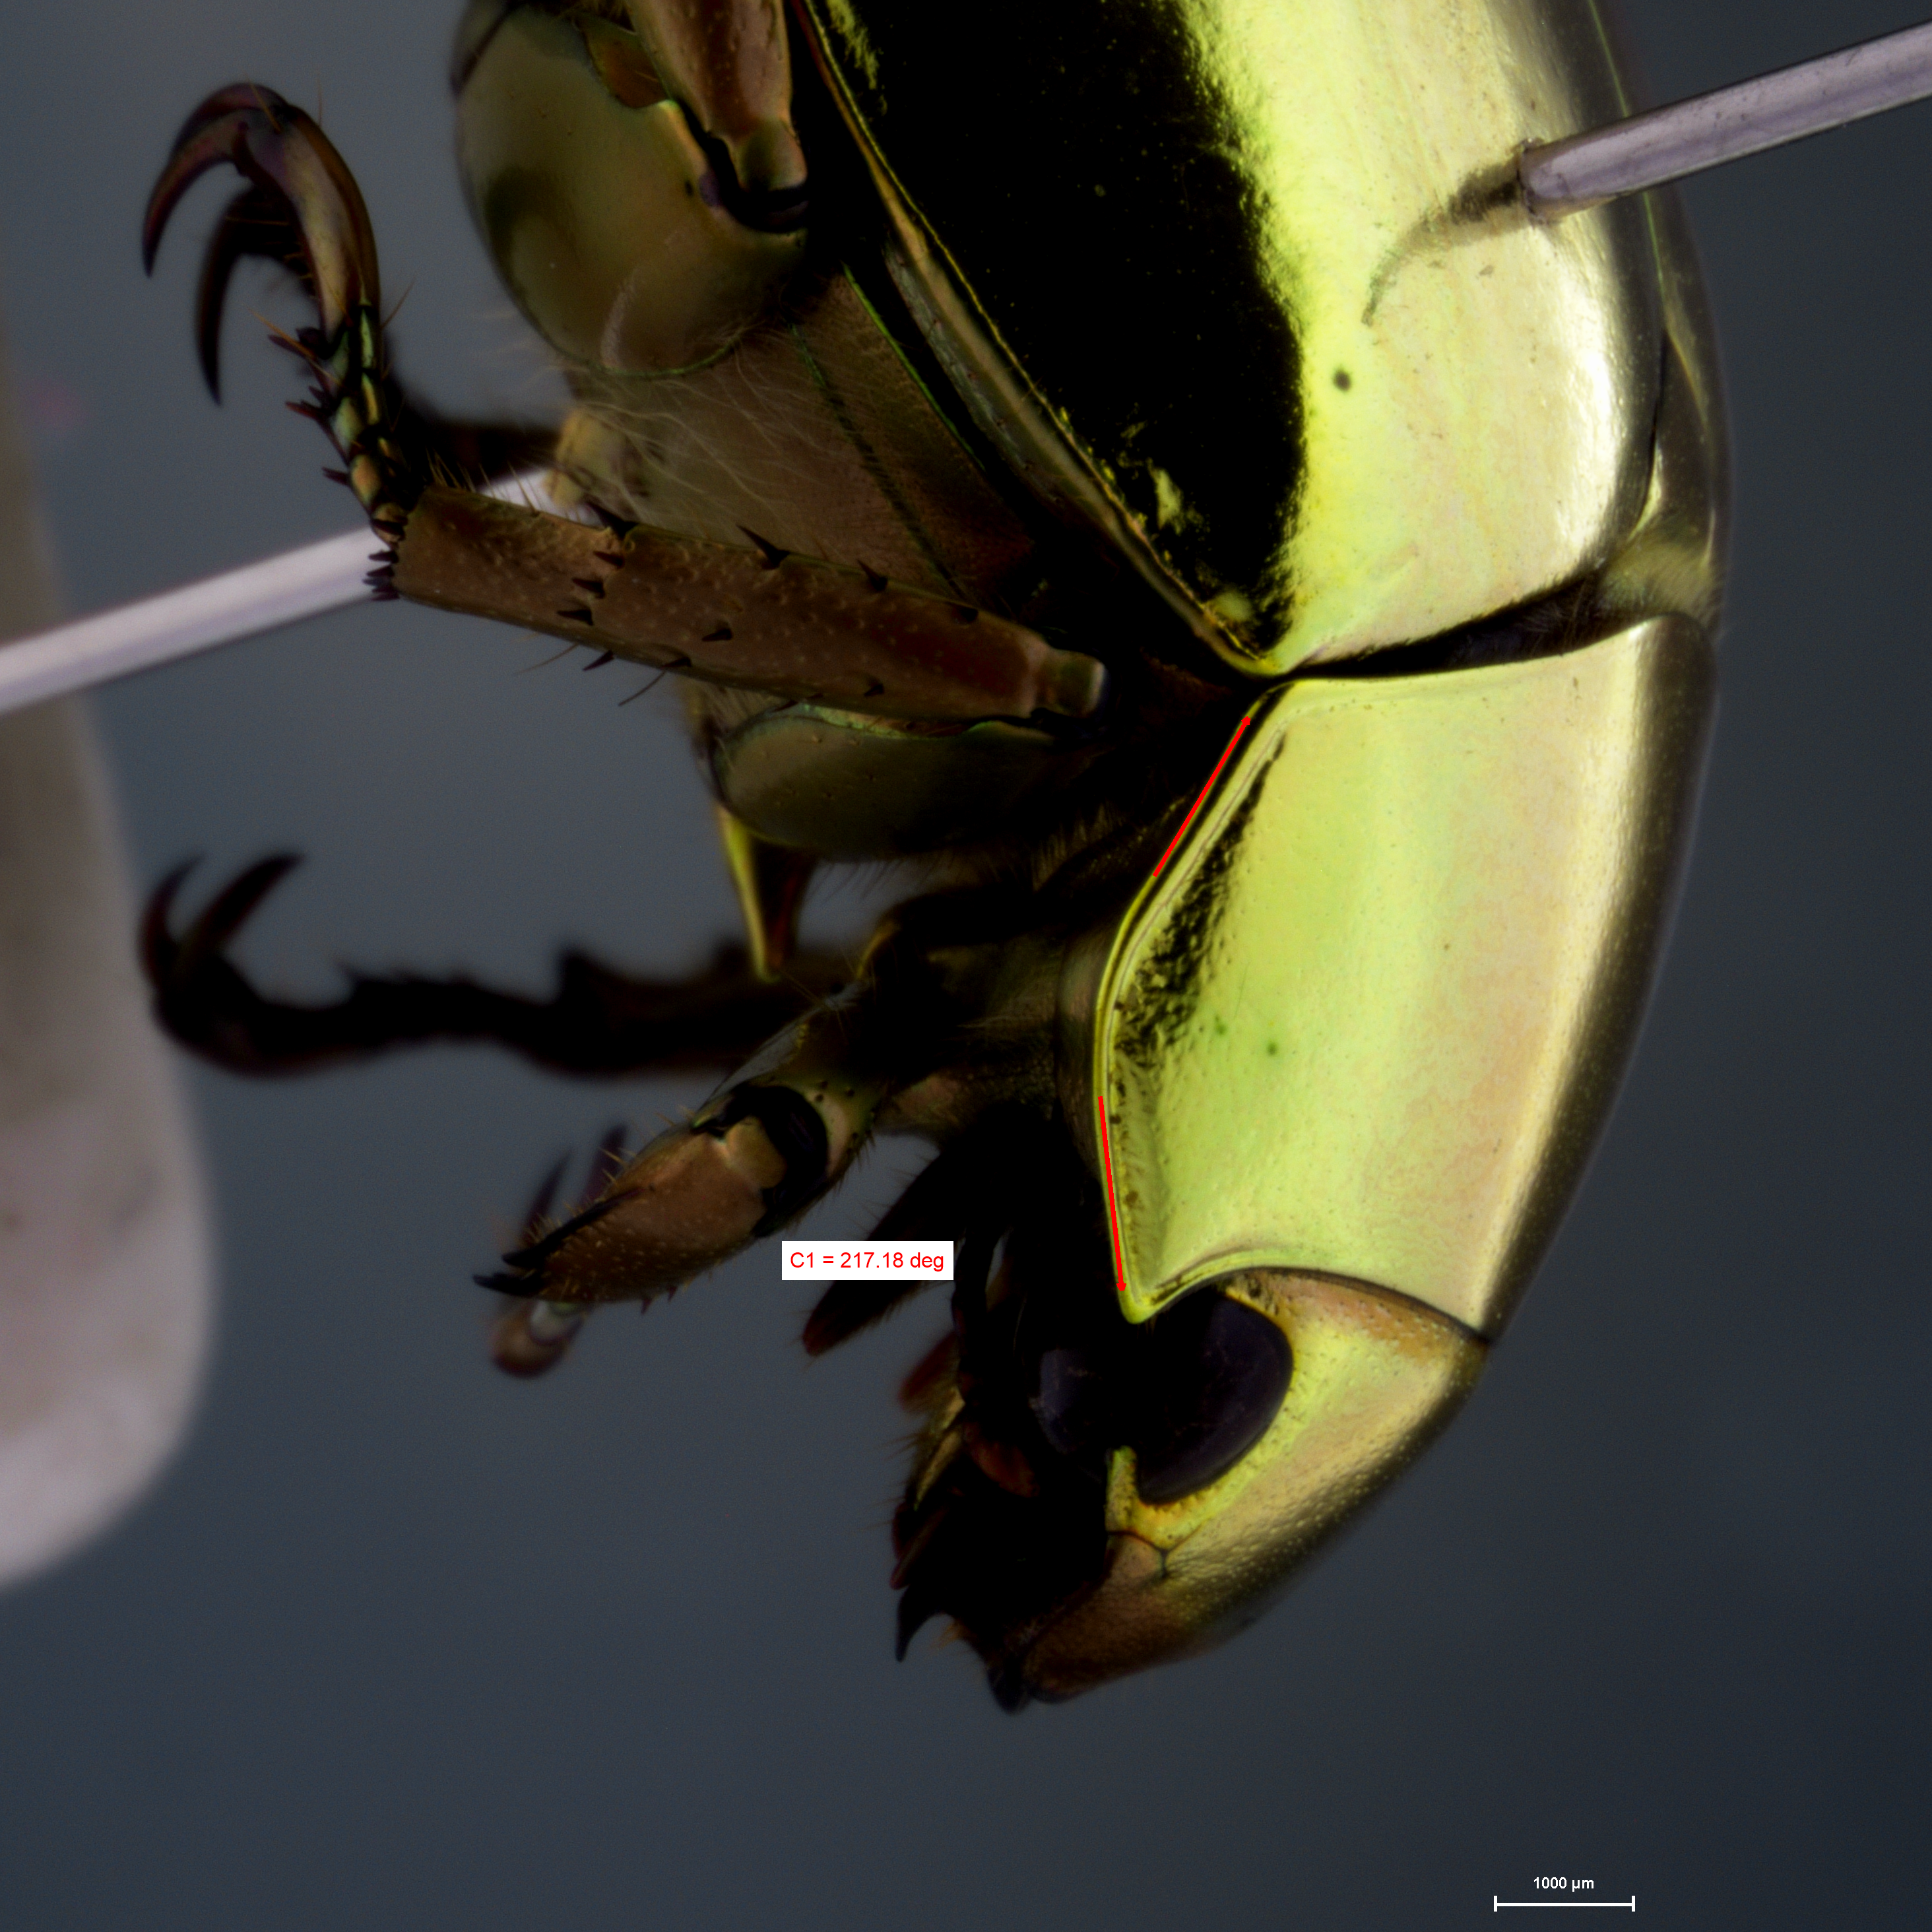
\includegraphics[width=0.5\linewidth]{images/protocol/Lateral_C1.png}
\caption{ Metric C1}
\end{figure}

\newpage
\subsection*{Metric: D1}

Mesosternal process’ horizontal length measured from the secant point of the tangents of its sides with the horizontal line used to measure D1. 

\begin{figure}[H]
\centering
\includegraphics[width=0.7\linewidth]{images/boxplot/boxplot_D1.png}
\caption{  Boxplot and specimen distribution (superposed) for the metric  D1 by species}
\end{figure}

\noindent\textbf{Test Type:} Student's t-test \\
\noindent\textbf{Test Statistic:} -1.458 \\
\noindent\textbf{P-value:} 0.155 \\
\noindent\textbf{Interpretation:} no significant difference

\begin{figure}[H]
\centering
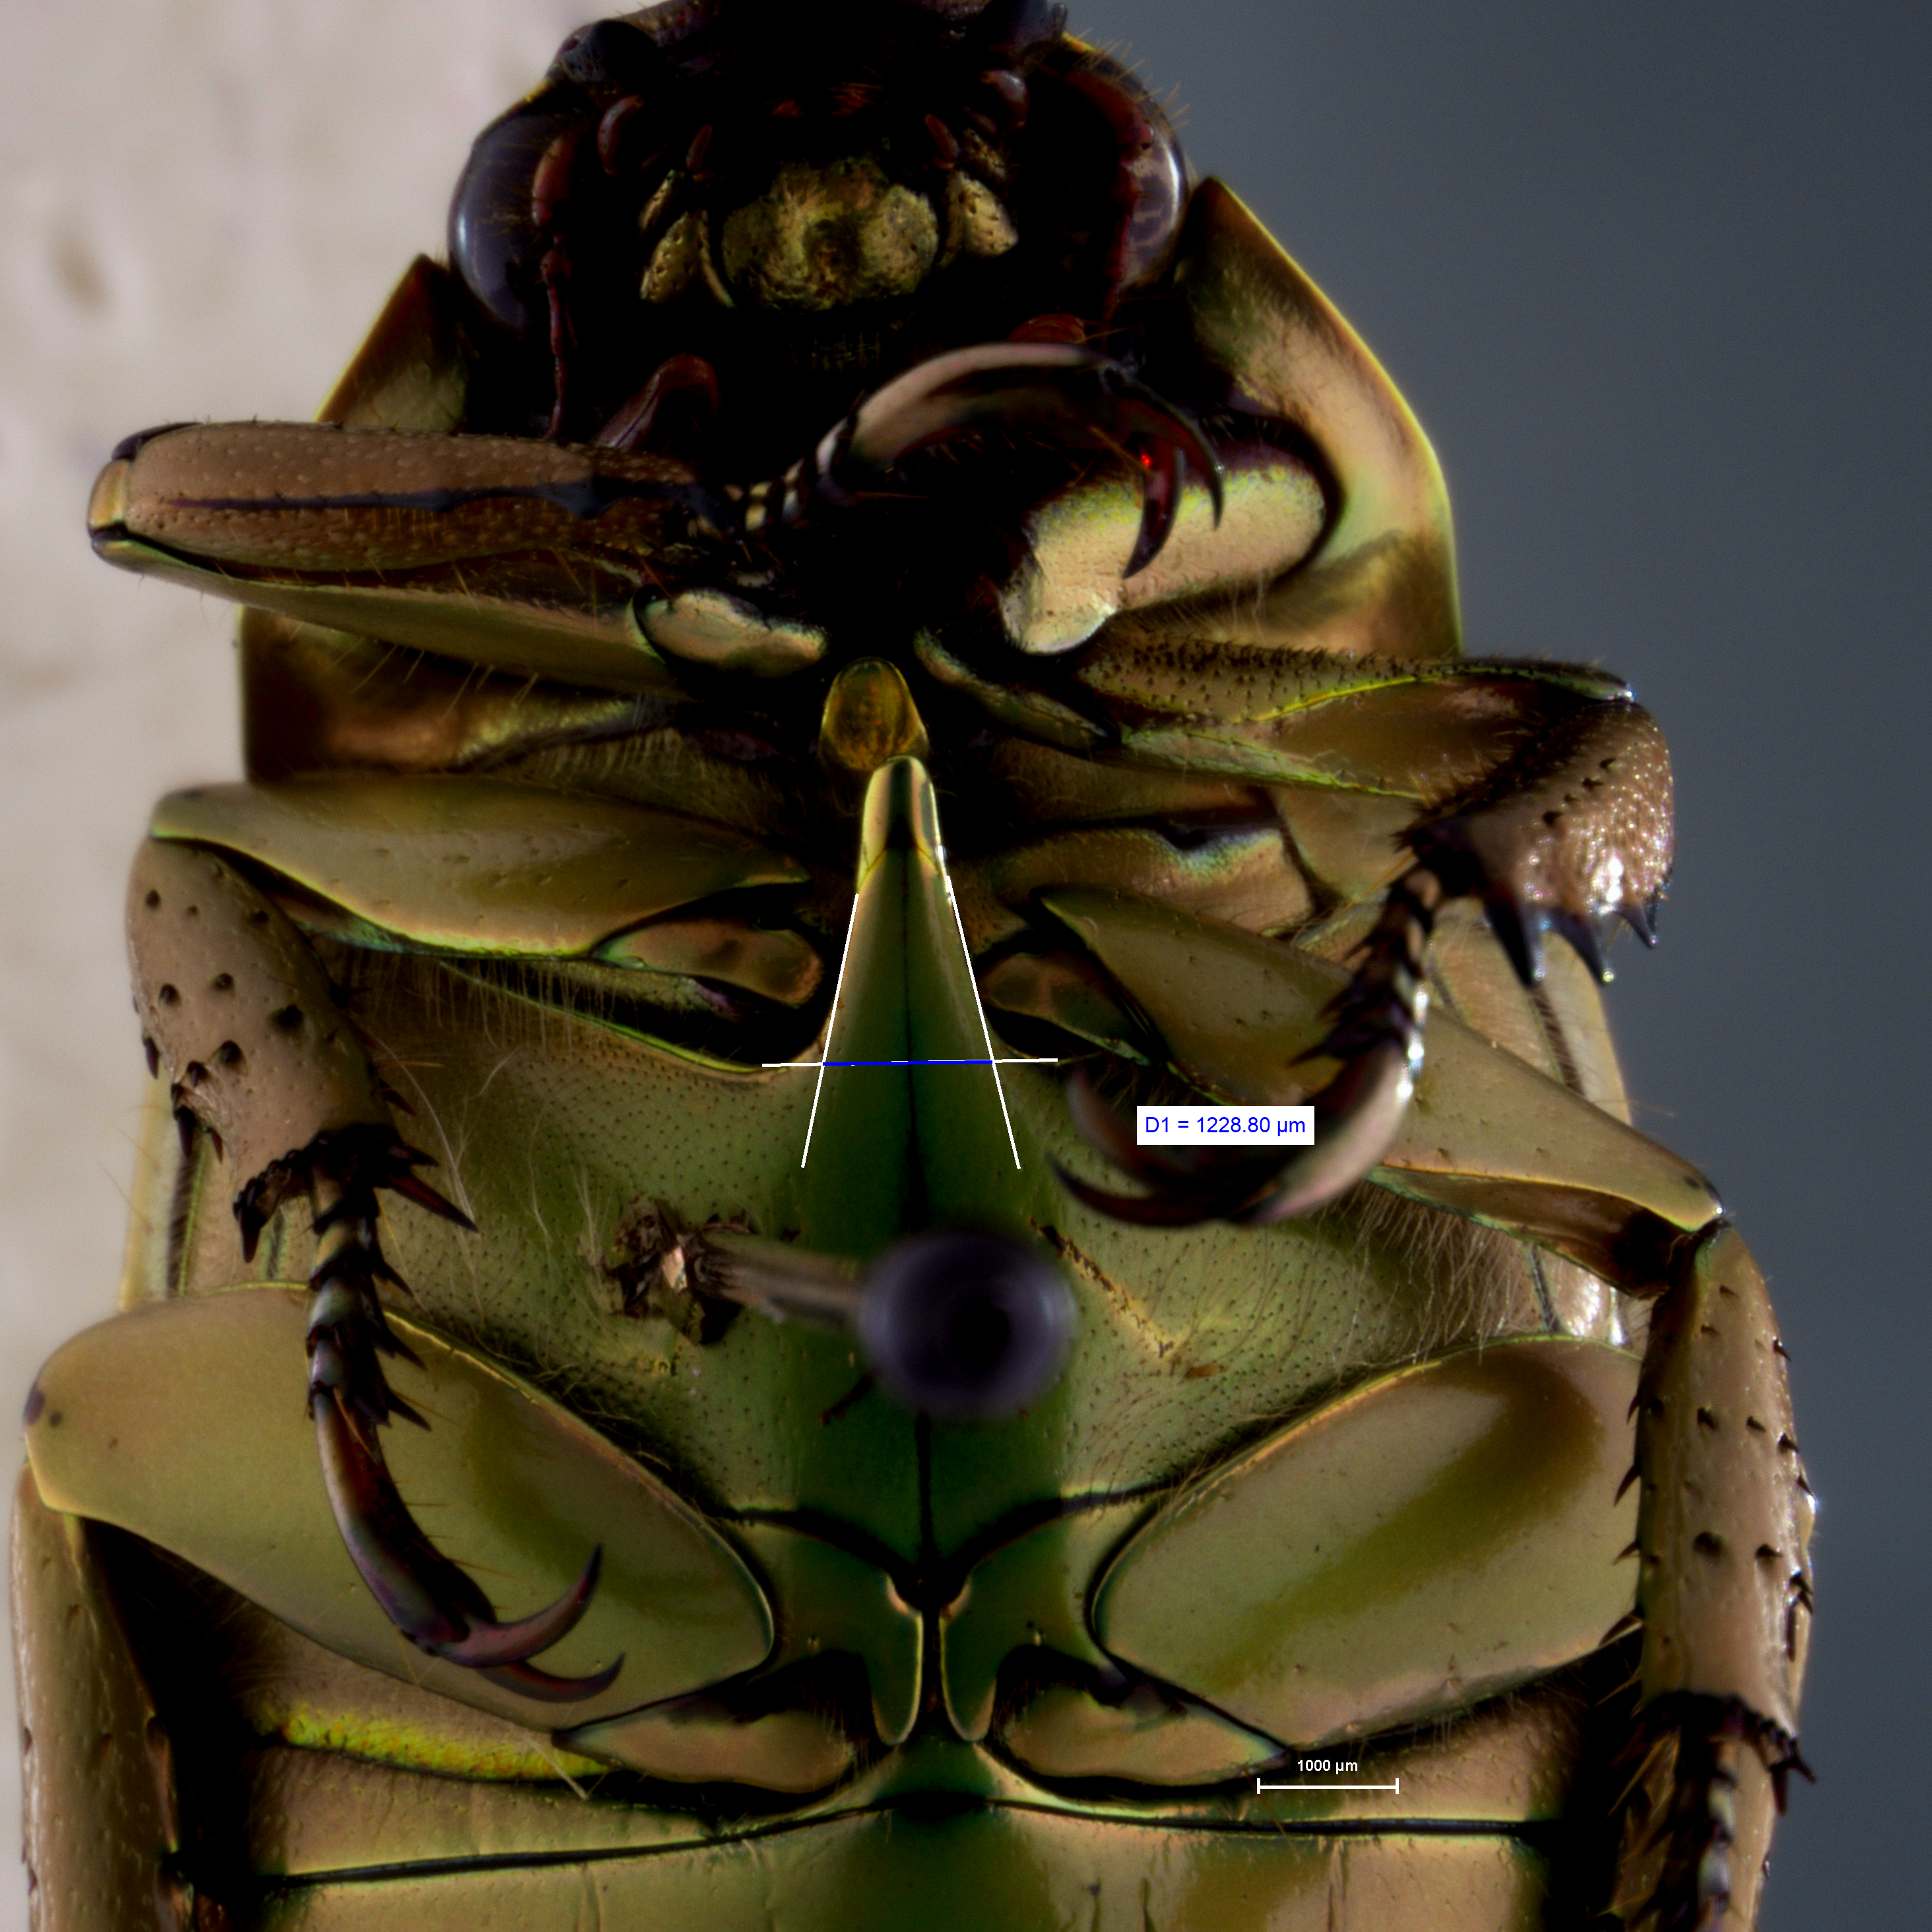
\includegraphics[width=0.5\linewidth]{images/protocol/Mesosternal_process_D1.png}
\caption{ Metric D1}
\end{figure}

\newpage
\subsection*{Metric: D2}

Mesosternal process’ vertical length measured from the tip of the mesosternal process down to the line that joins the two lowest curves at the sides of the mesosternal process base

\begin{figure}[H]
\centering
\includegraphics[width=0.7\linewidth]{images/boxplot/boxplot_D2.png}
\caption{  Boxplot and specimen distribution (superposed) for the metric  D2 by species}
\end{figure}

\noindent\textbf{Test Type:} Student's t-test \\
\noindent\textbf{Test Statistic:} -0.647 \\
\noindent\textbf{P-value:} 0.522 \\
\noindent\textbf{Interpretation:} no significant difference

\begin{figure}[H]
\centering
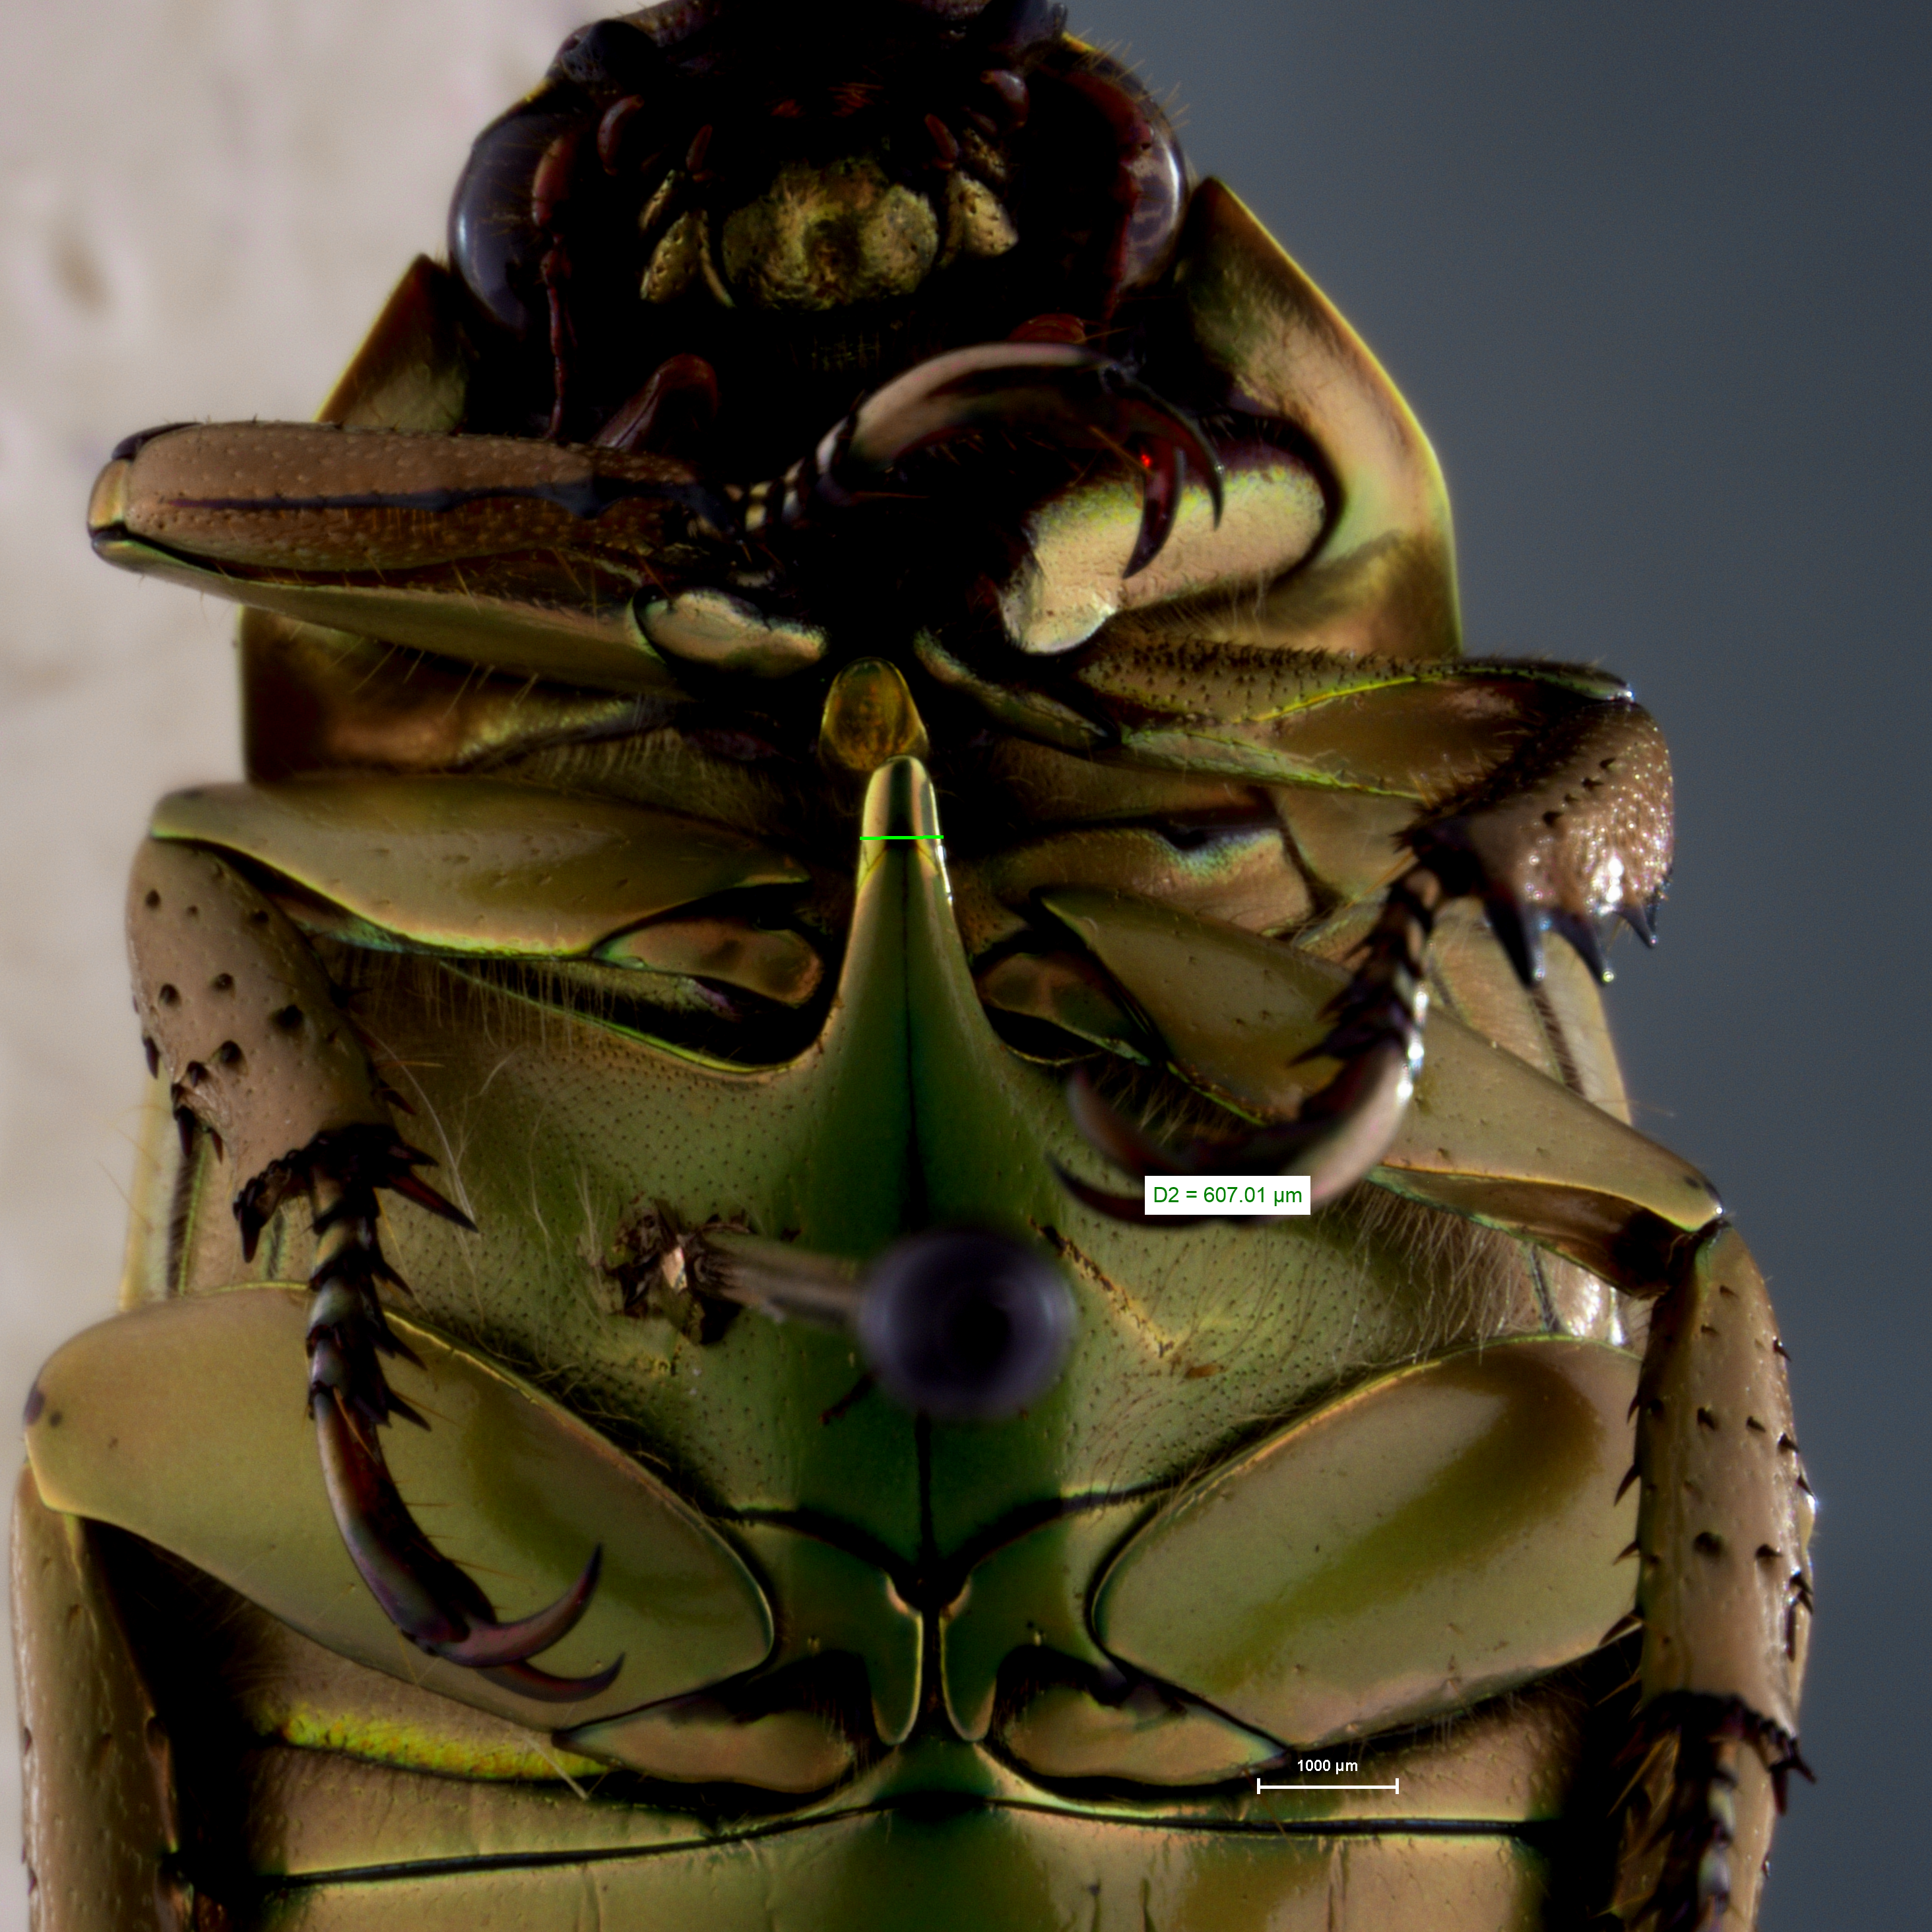
\includegraphics[width=0.5\linewidth]{images/protocol/Mesosternal_process_D2.png}
\caption{ Metric D2}
\end{figure}

\newpage
\subsection*{Metric: D3}

Horizontal width of the dark middle line measured from its two lower ends

\begin{figure}[H]
\centering
\includegraphics[width=0.7\linewidth]{images/boxplot/boxplot_D3.png}
\caption{  Boxplot and specimen distribution (superposed) for the metric  D3 by species}
\end{figure}

\noindent\textbf{Test Type:} Student's t-test \\
\noindent\textbf{Test Statistic:} -1.148 \\
\noindent\textbf{P-value:} 0.260 \\
\noindent\textbf{Interpretation:} no significant difference

\begin{figure}[H]
\centering
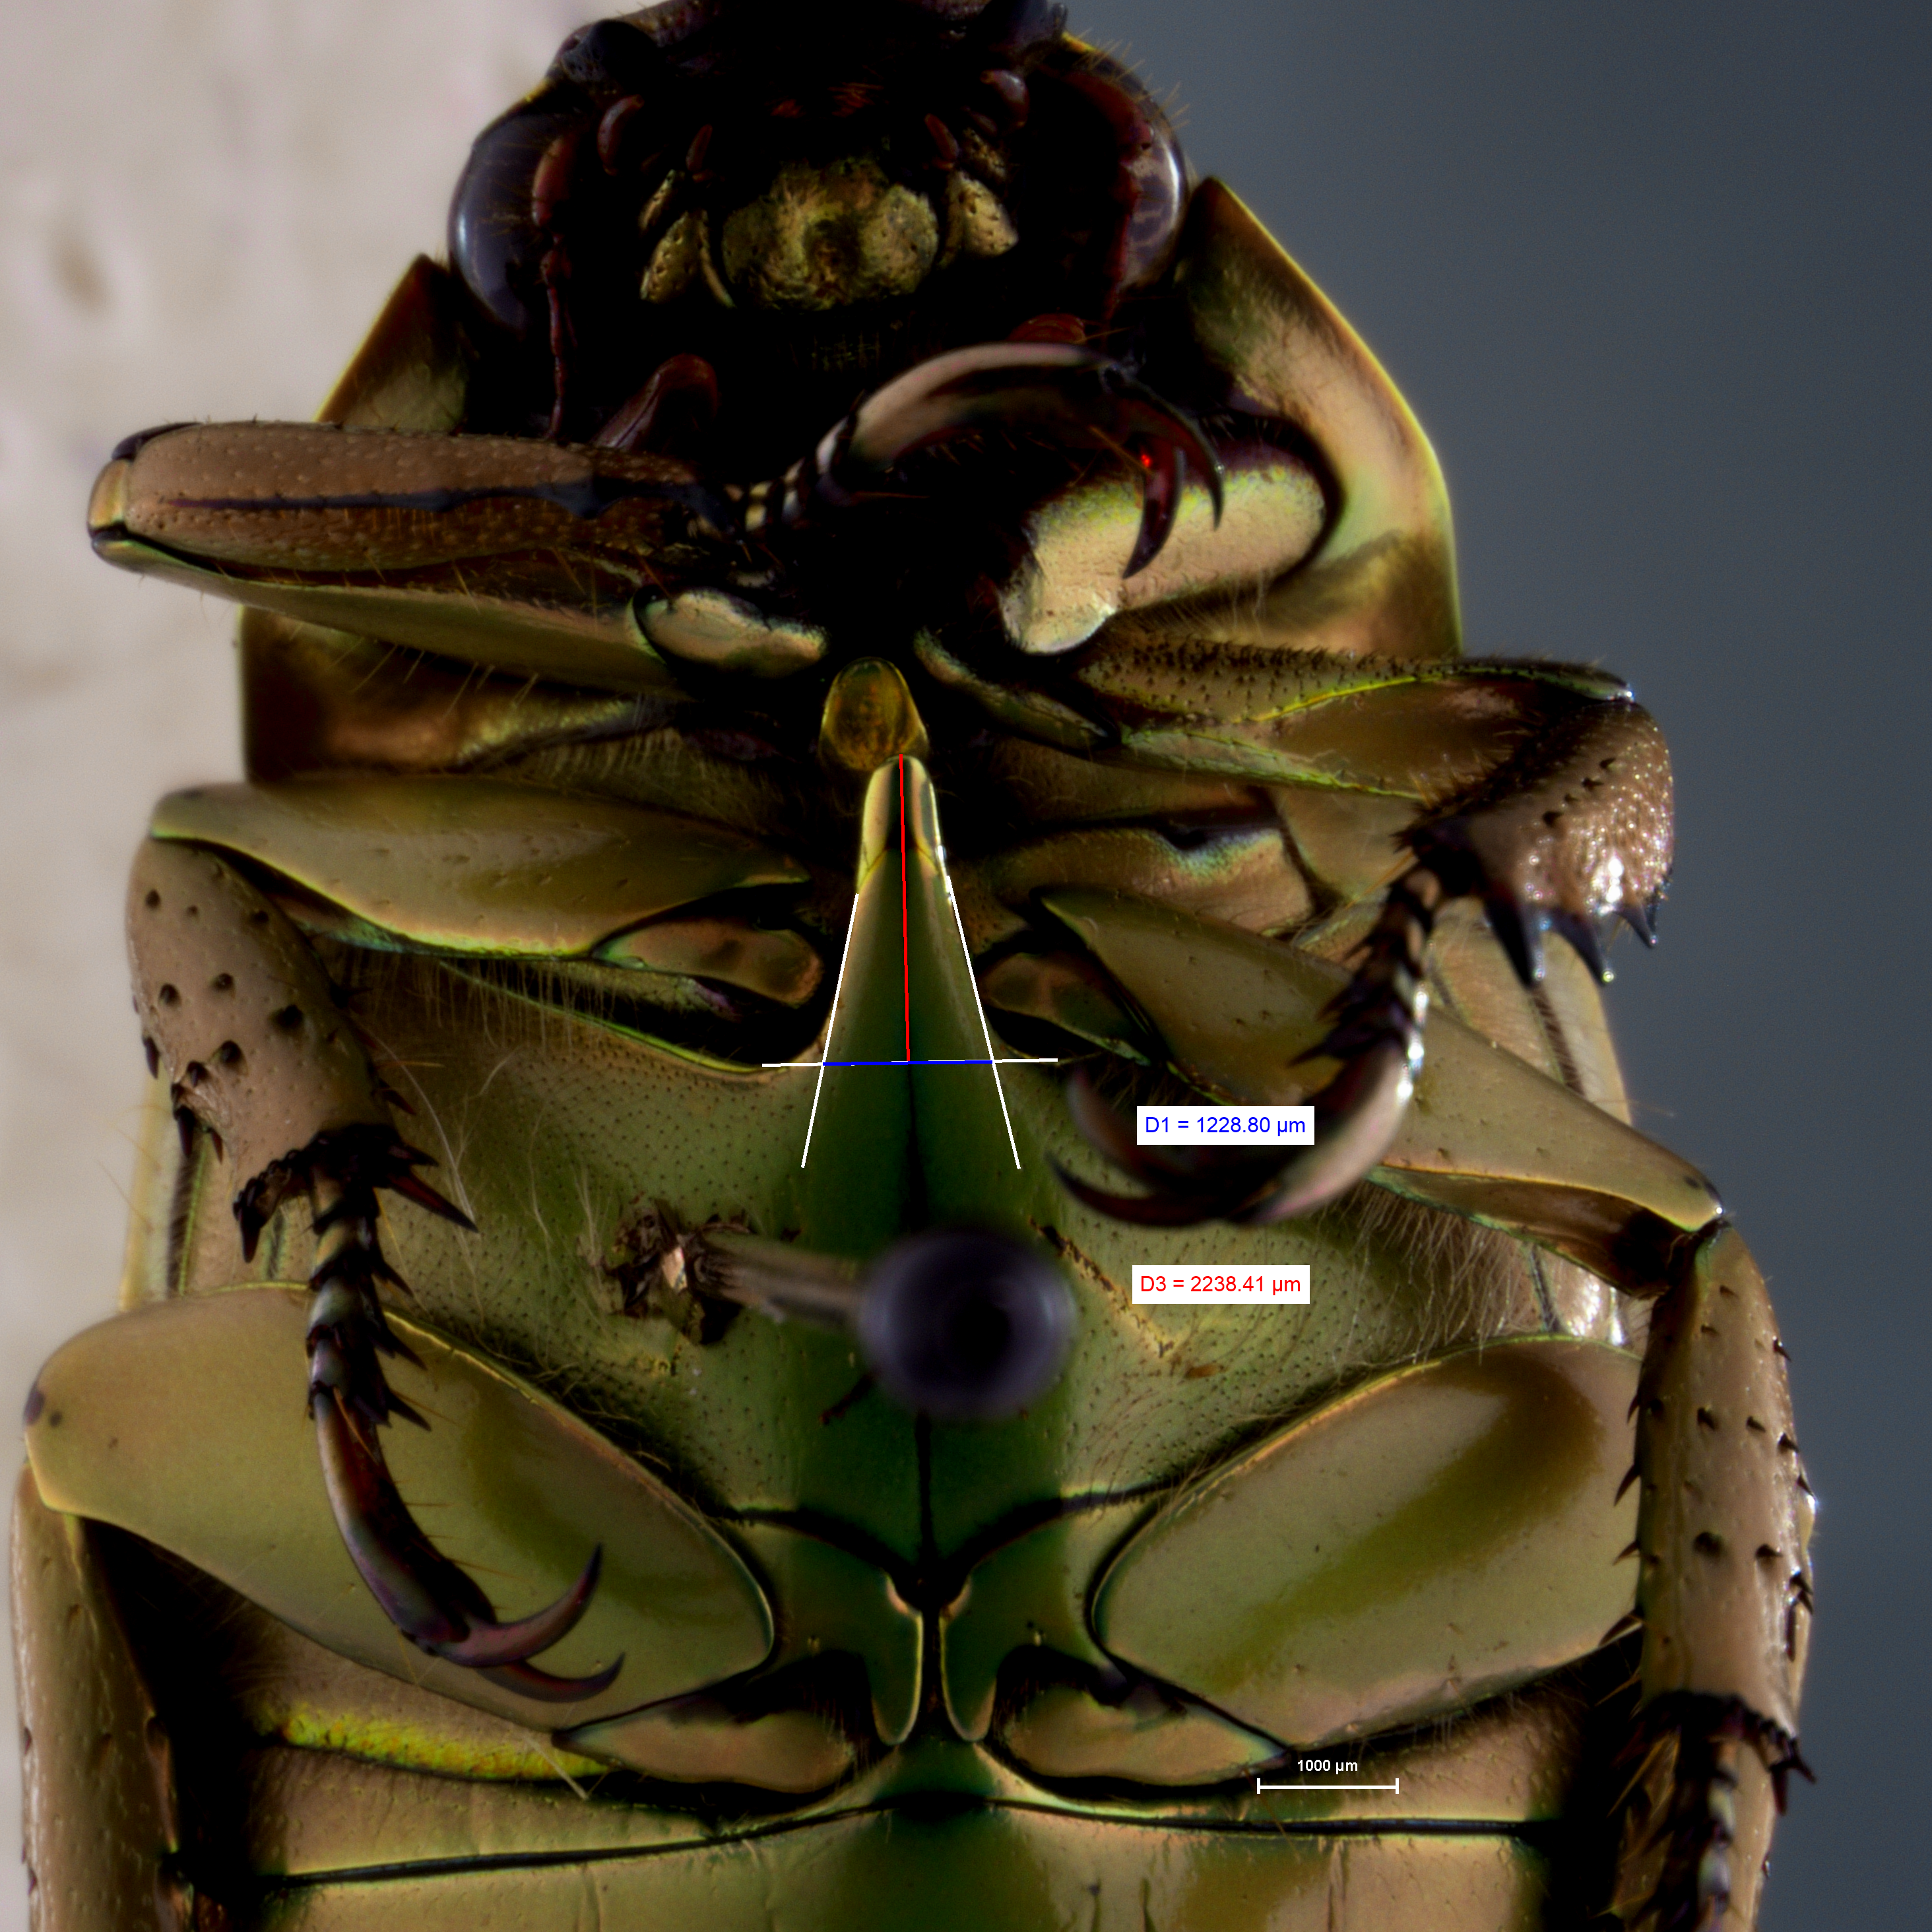
\includegraphics[width=0.5\linewidth]{images/protocol/Mesosternal_process_D3.png}
\caption{ Metric D3}
\end{figure}

\newpage
\subsection*{Metric: D4}

Vertical length from the tip of the mesosternal process down to the lowest point of the black patch in the middle of the mesosternal process

\begin{figure}[H]
\centering
\includegraphics[width=0.7\linewidth]{images/boxplot/boxplot_D4.png}
\caption{  Boxplot and specimen distribution (superposed) for the metric  D4 by species}
\end{figure}

\noindent\textbf{Test Type:} Student's t-test \\
\noindent\textbf{Test Statistic:} -2.552 \\
\noindent\textbf{P-value:} 0.016 \\
\noindent\textbf{Interpretation:} significant difference

\begin{figure}[H]
\centering
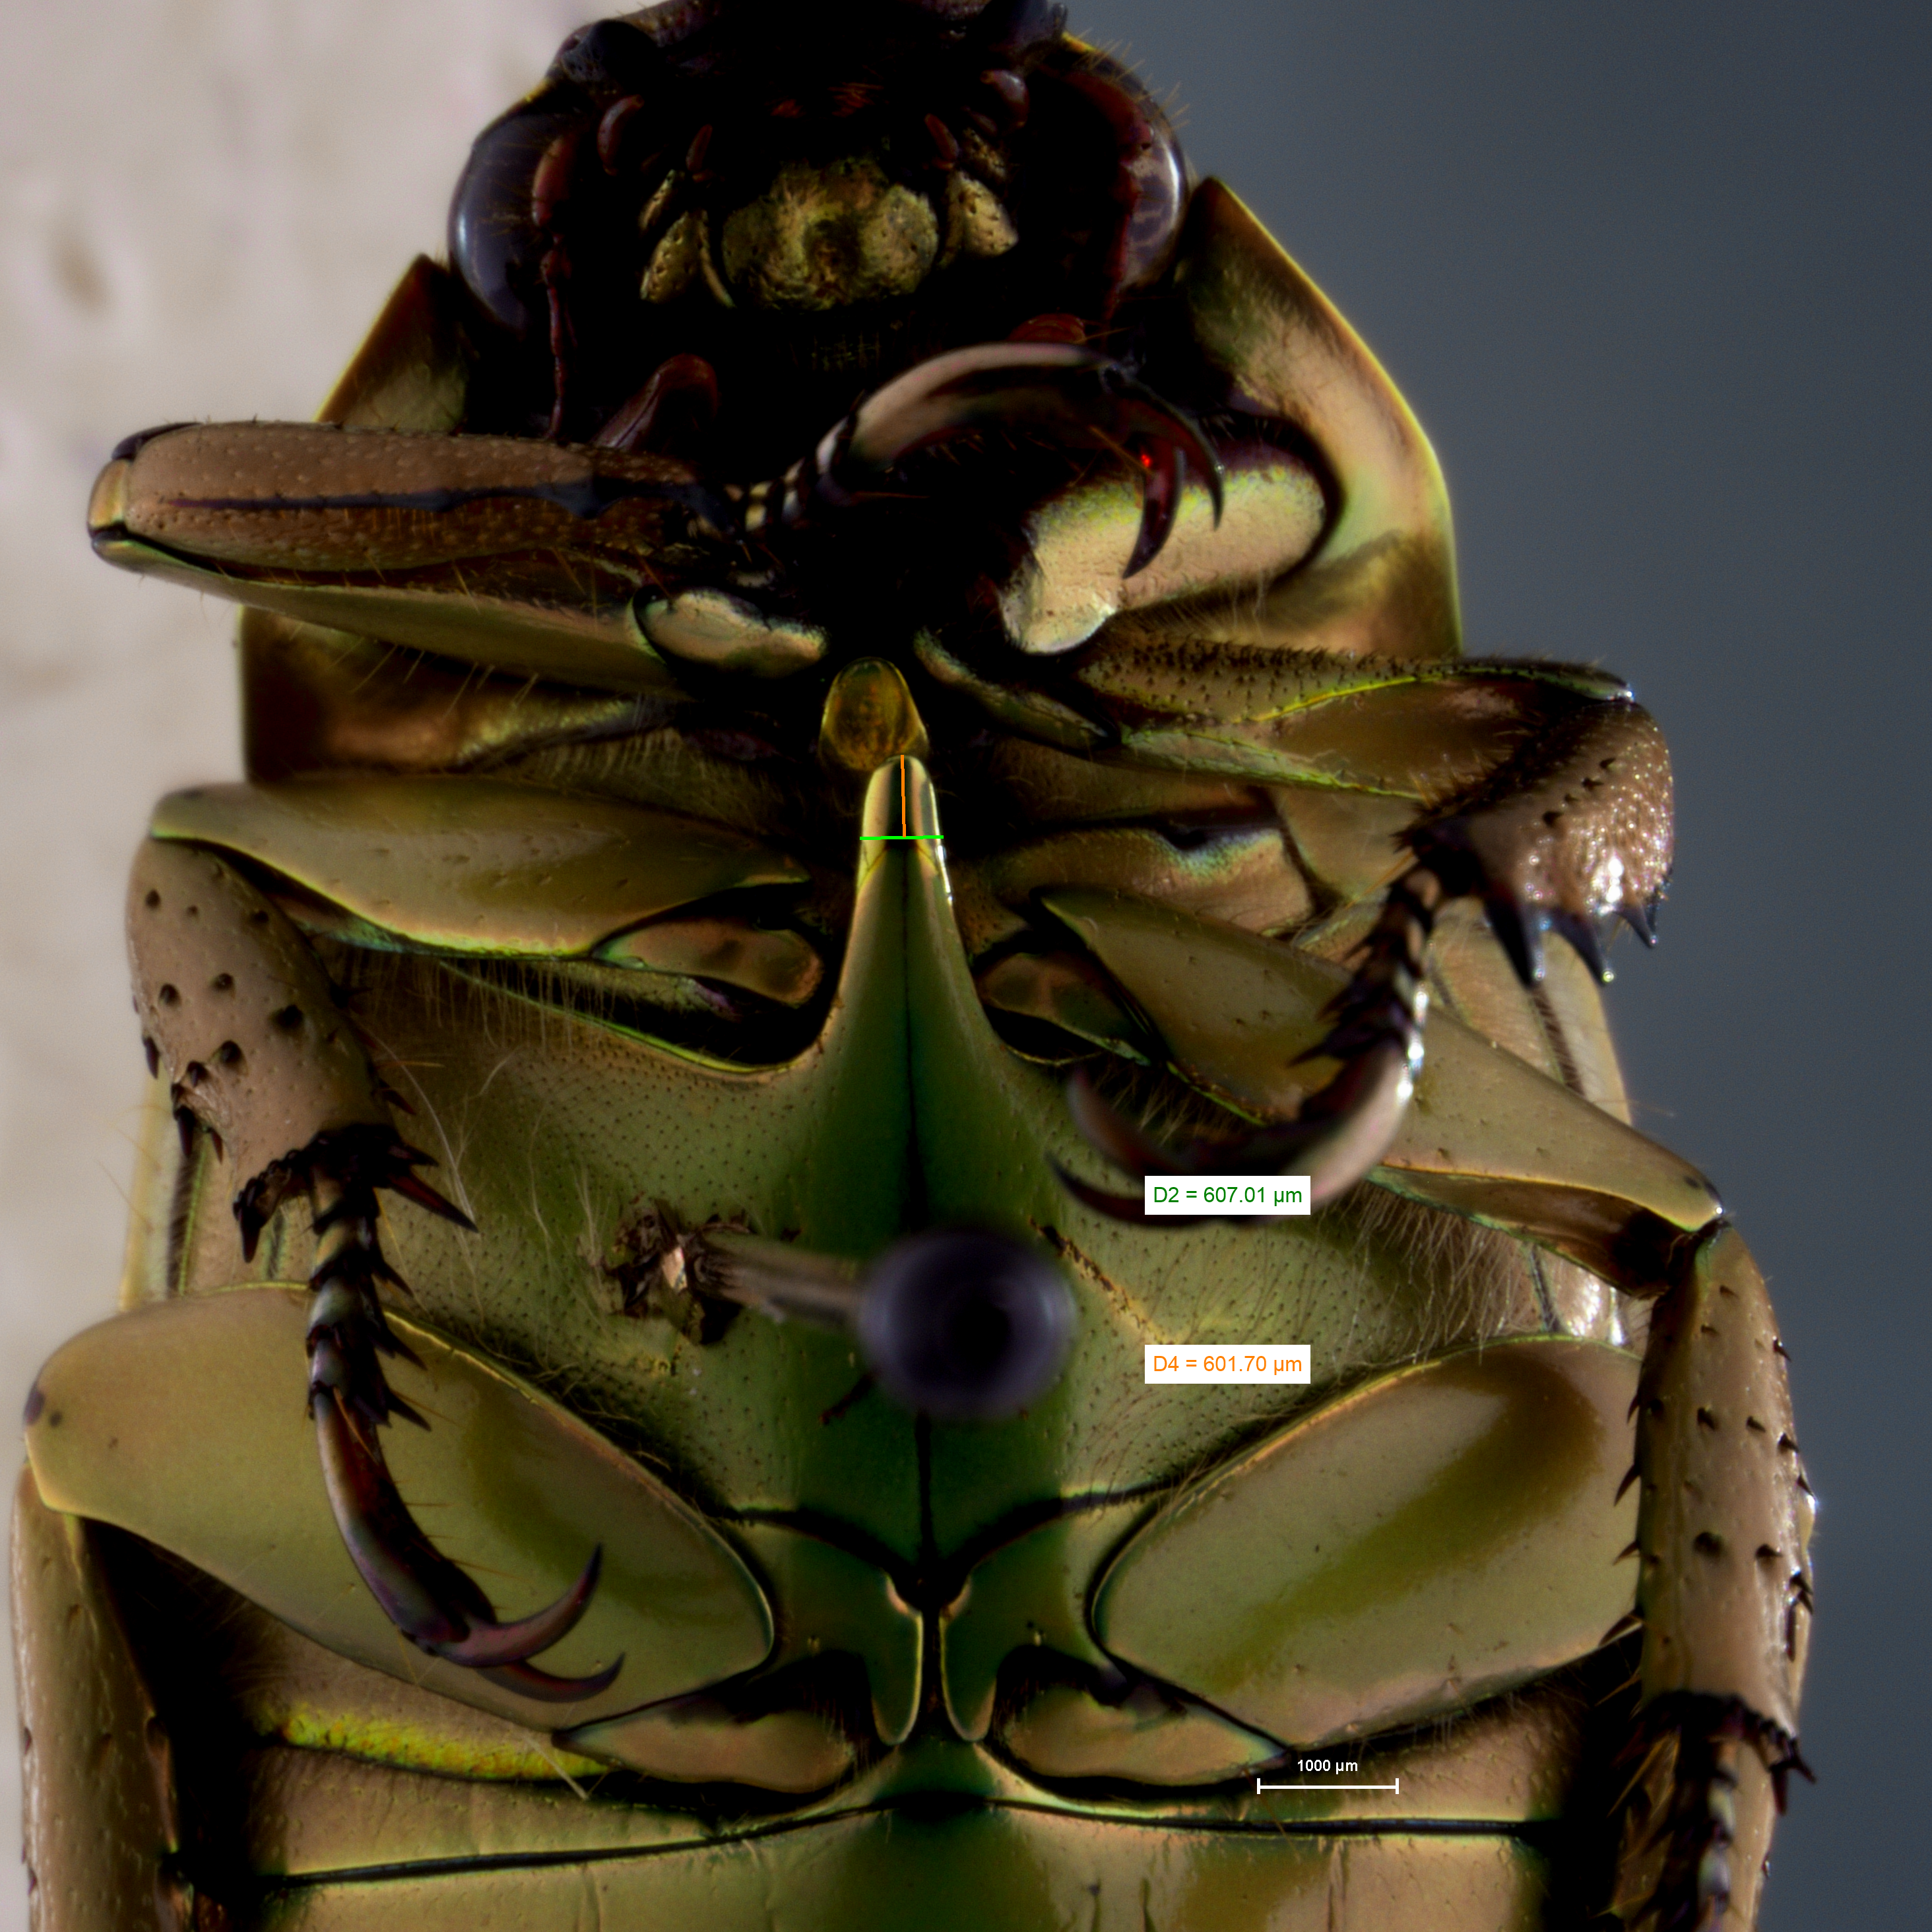
\includegraphics[width=0.5\linewidth]{images/protocol/Mesosternal_process_D4.png}
\caption{ Metric D4}
\end{figure}

\newpage
\subsection*{Metric: E1}

Horizontal top width of the prosternal plate 

\begin{figure}[H]
\centering
\includegraphics[width=0.7\linewidth]{images/boxplot/boxplot_E1.png}
\caption{  Boxplot and specimen distribution (superposed) for the metric  E1 by species}
\end{figure}

\noindent\textbf{Test Type:} Student's t-test \\
\noindent\textbf{Test Statistic:} -2.453 \\
\noindent\textbf{P-value:} 0.020 \\
\noindent\textbf{Interpretation:} significant difference

\begin{figure}[H]
\centering
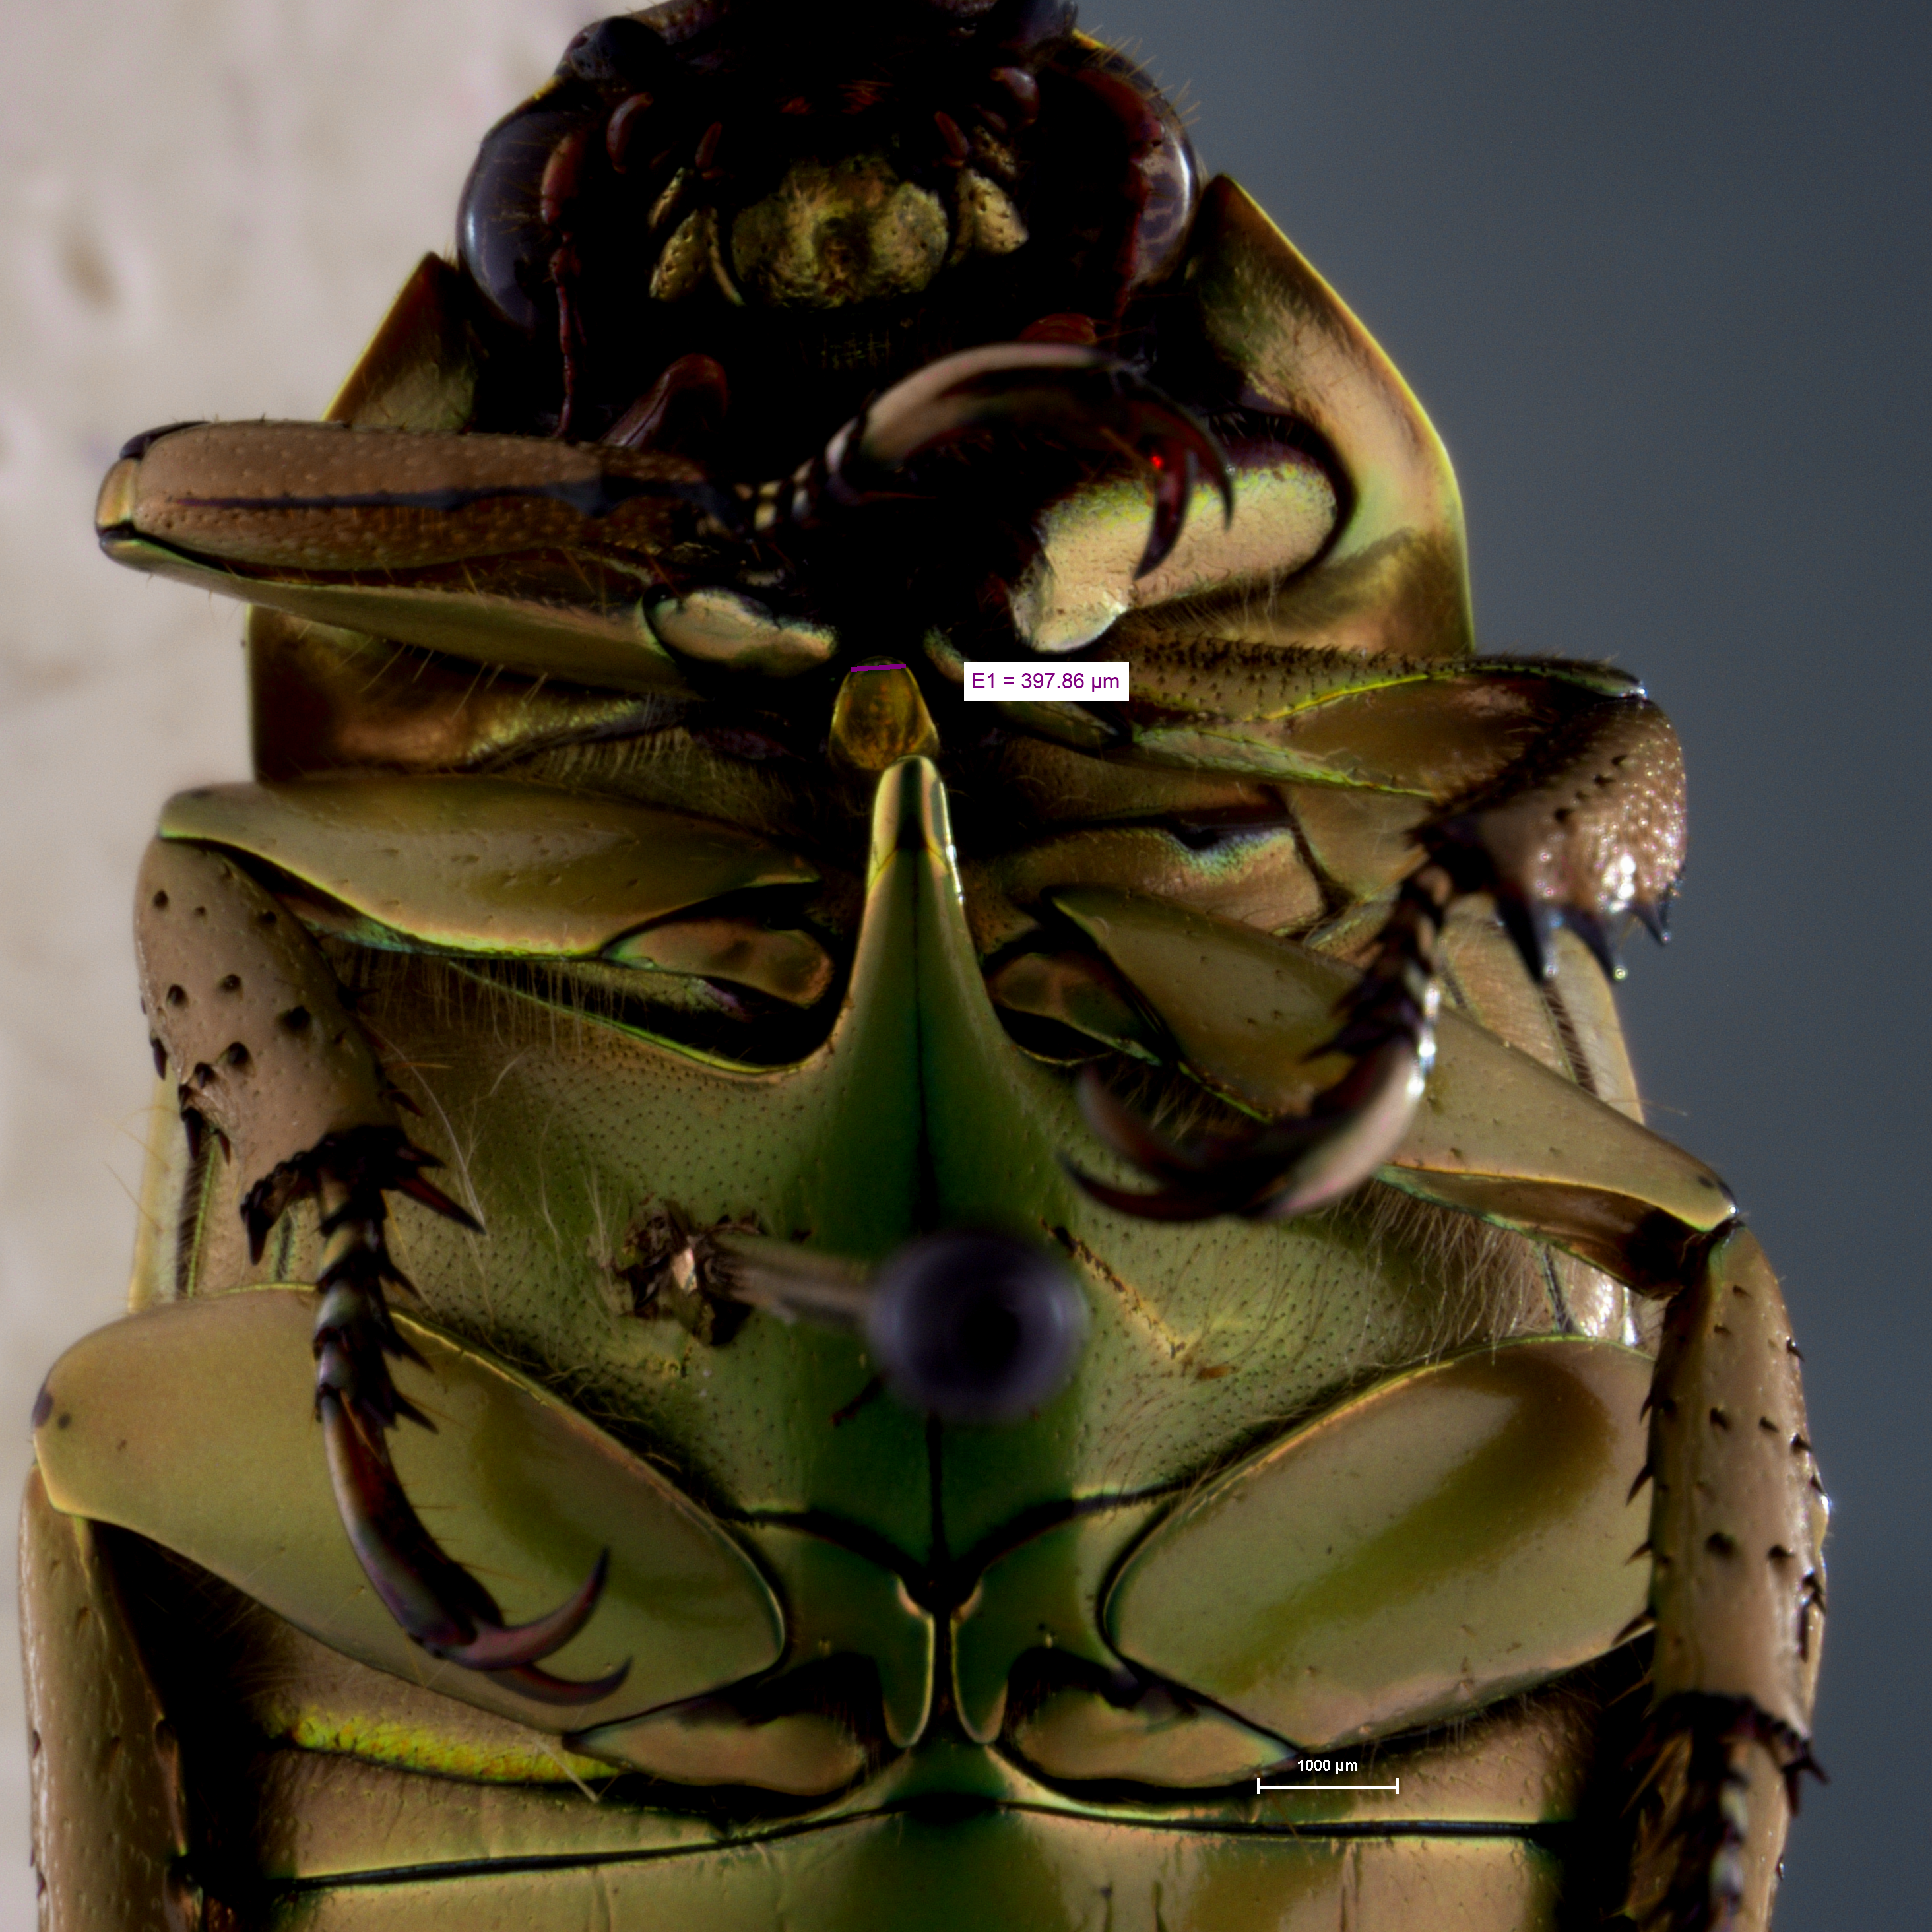
\includegraphics[width=0.5\linewidth]{images/protocol/Prosternal_process_E1.png}
\caption{ Metric E1}
\end{figure}

\newpage
\subsection*{Metric: E2}

Horizontal bottom width of the prosternal plate 

\begin{figure}[H]
\centering
\includegraphics[width=0.7\linewidth]{images/boxplot/boxplot_E2.png}
\caption{  Boxplot and specimen distribution (superposed) for the metric  E2 by species}
\end{figure}

\noindent\textbf{Test Type:} Mann-Whitney U test \\
\noindent\textbf{Test Statistic:} 124.000 \\
\noindent\textbf{P-value:} 0.941 \\
\noindent\textbf{Interpretation:} no significant difference

\begin{figure}[H]
\centering
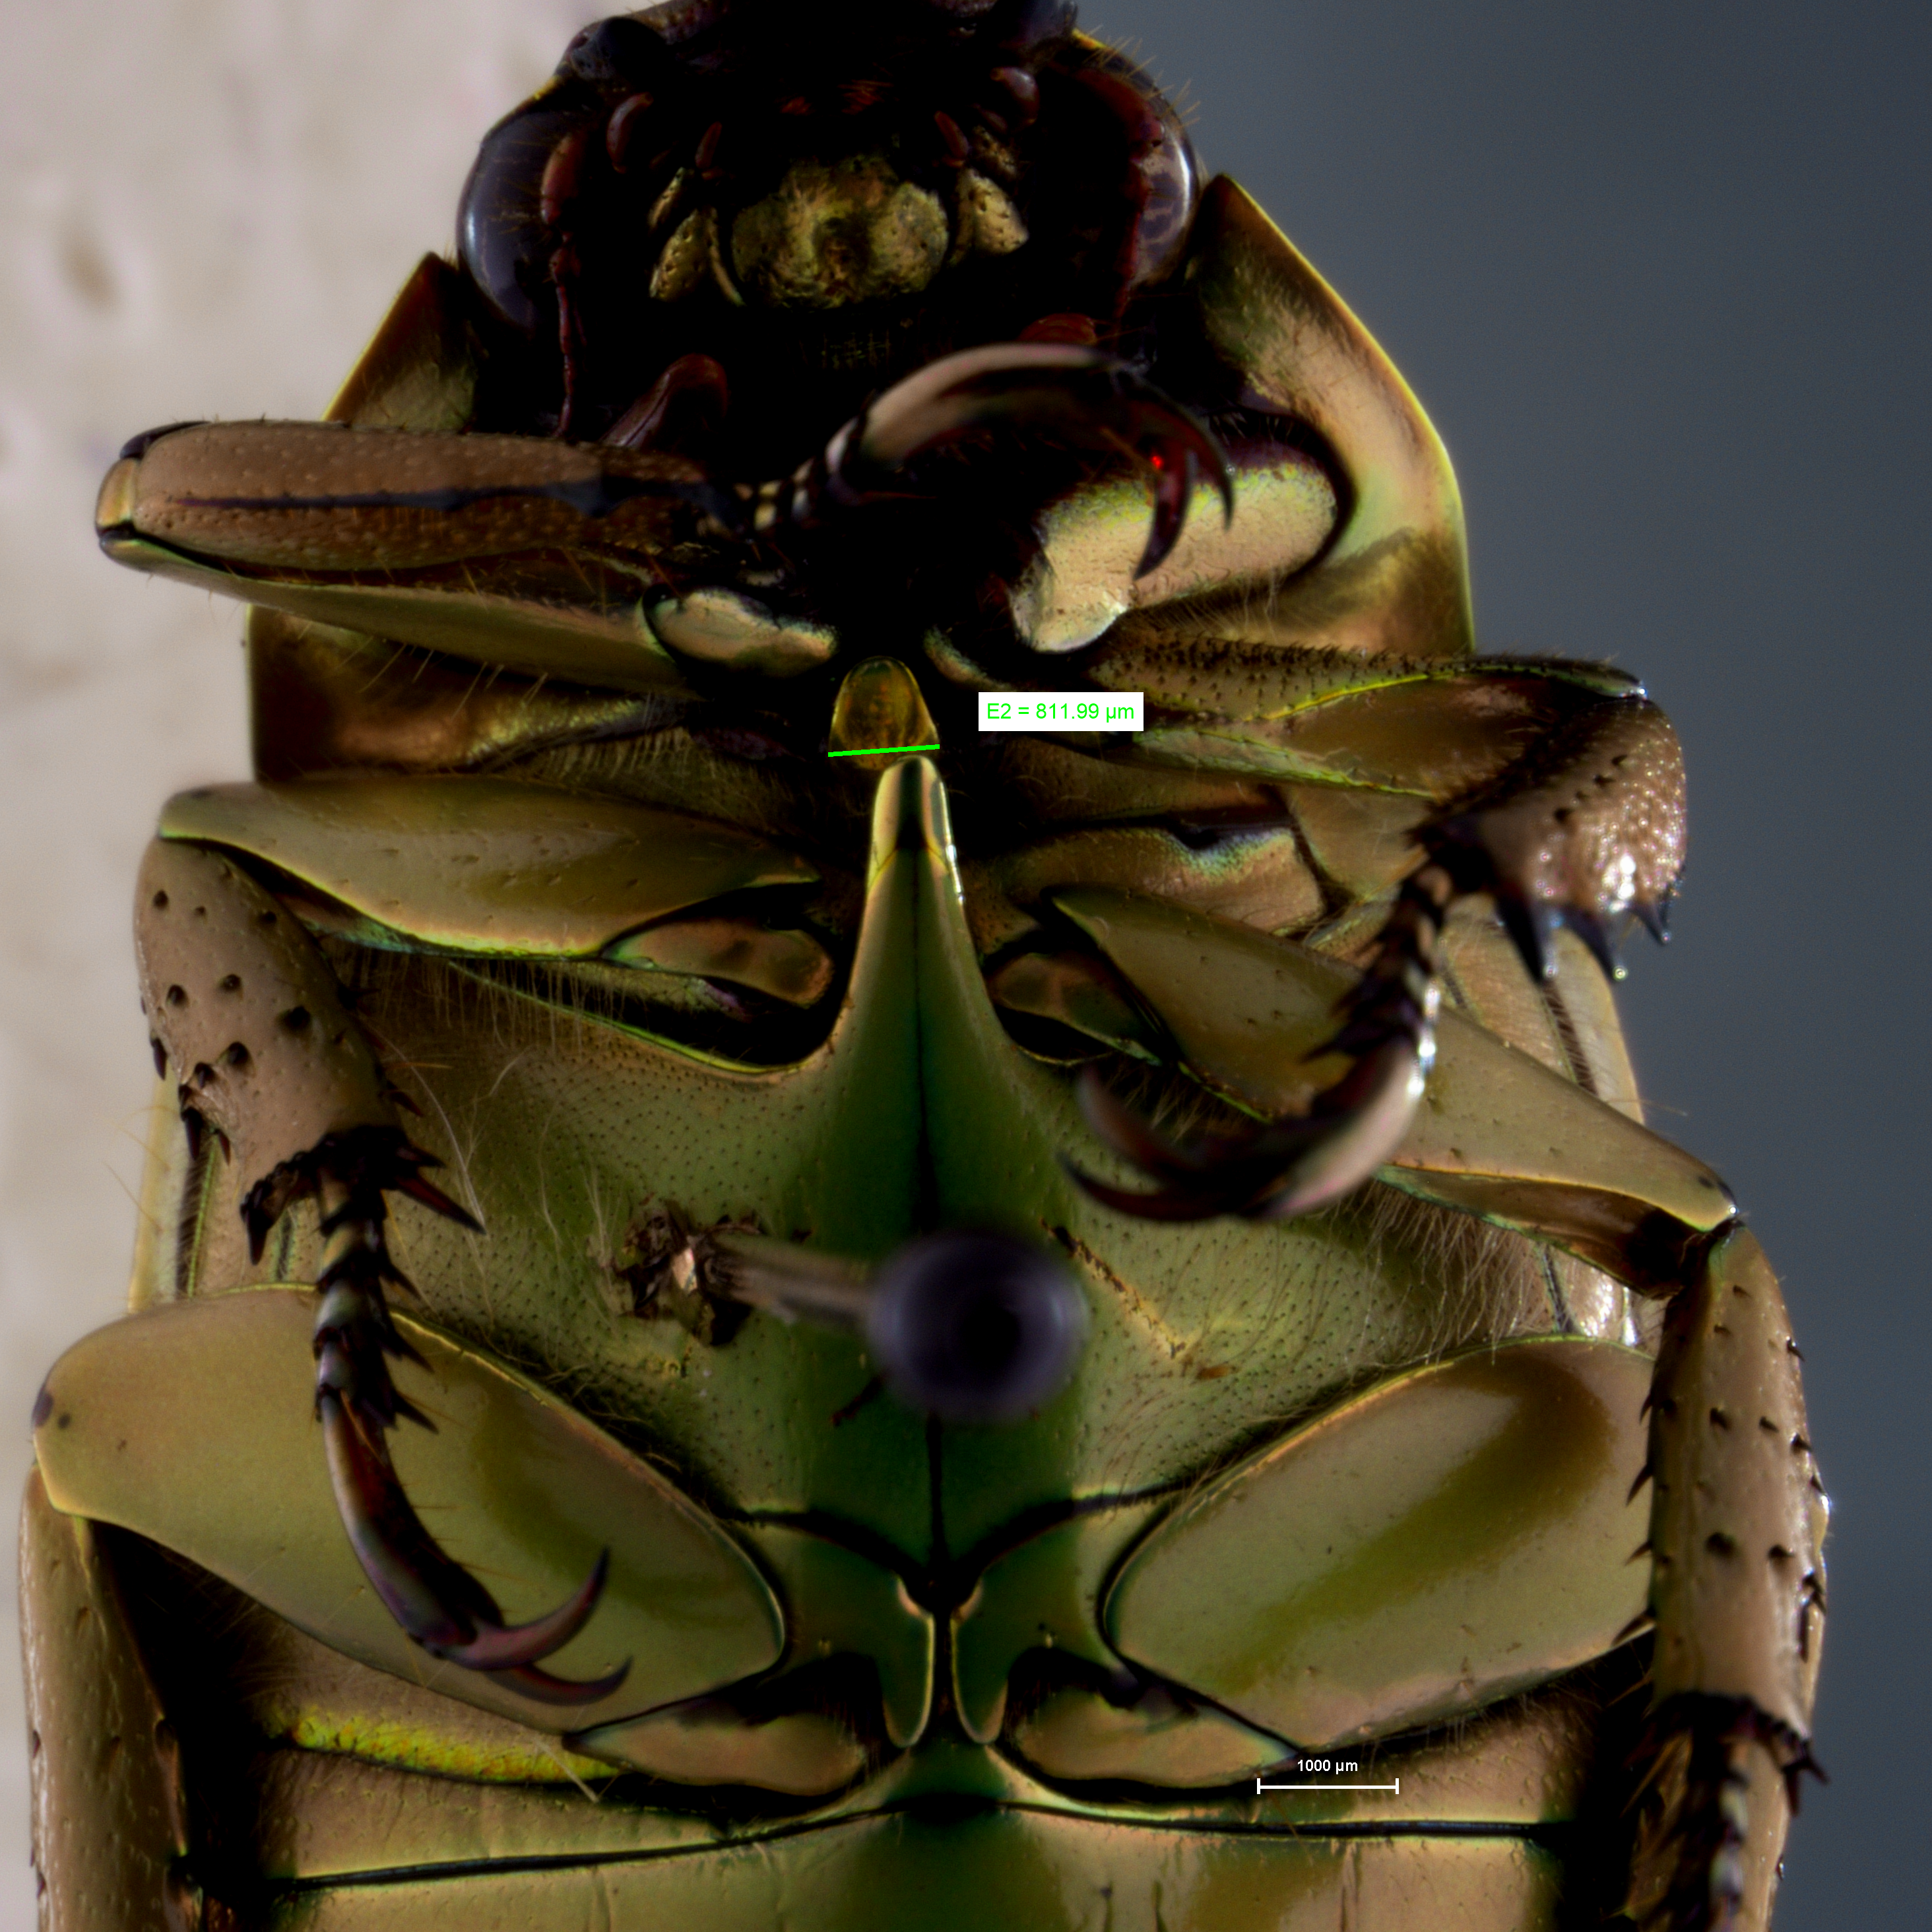
\includegraphics[width=0.5\linewidth]{images/protocol/Prosternal_process_E2.png}
\caption{ Metric E2}
\end{figure}

\newpage
\subsection*{Metric: F1}

Vertical length of the foremost ventral plate

\begin{figure}[H]
\centering
\includegraphics[width=0.7\linewidth]{images/boxplot/boxplot_F1.png}
\caption{  Boxplot and specimen distribution (superposed) for the metric  F1 by species}
\end{figure}

\noindent\textbf{Test Type:} Welch's t-test \\
\noindent\textbf{Test Statistic:} -2.665 \\
\noindent\textbf{P-value:} 0.012 \\
\noindent\textbf{Interpretation:} significant difference

\begin{figure}[H]
\centering
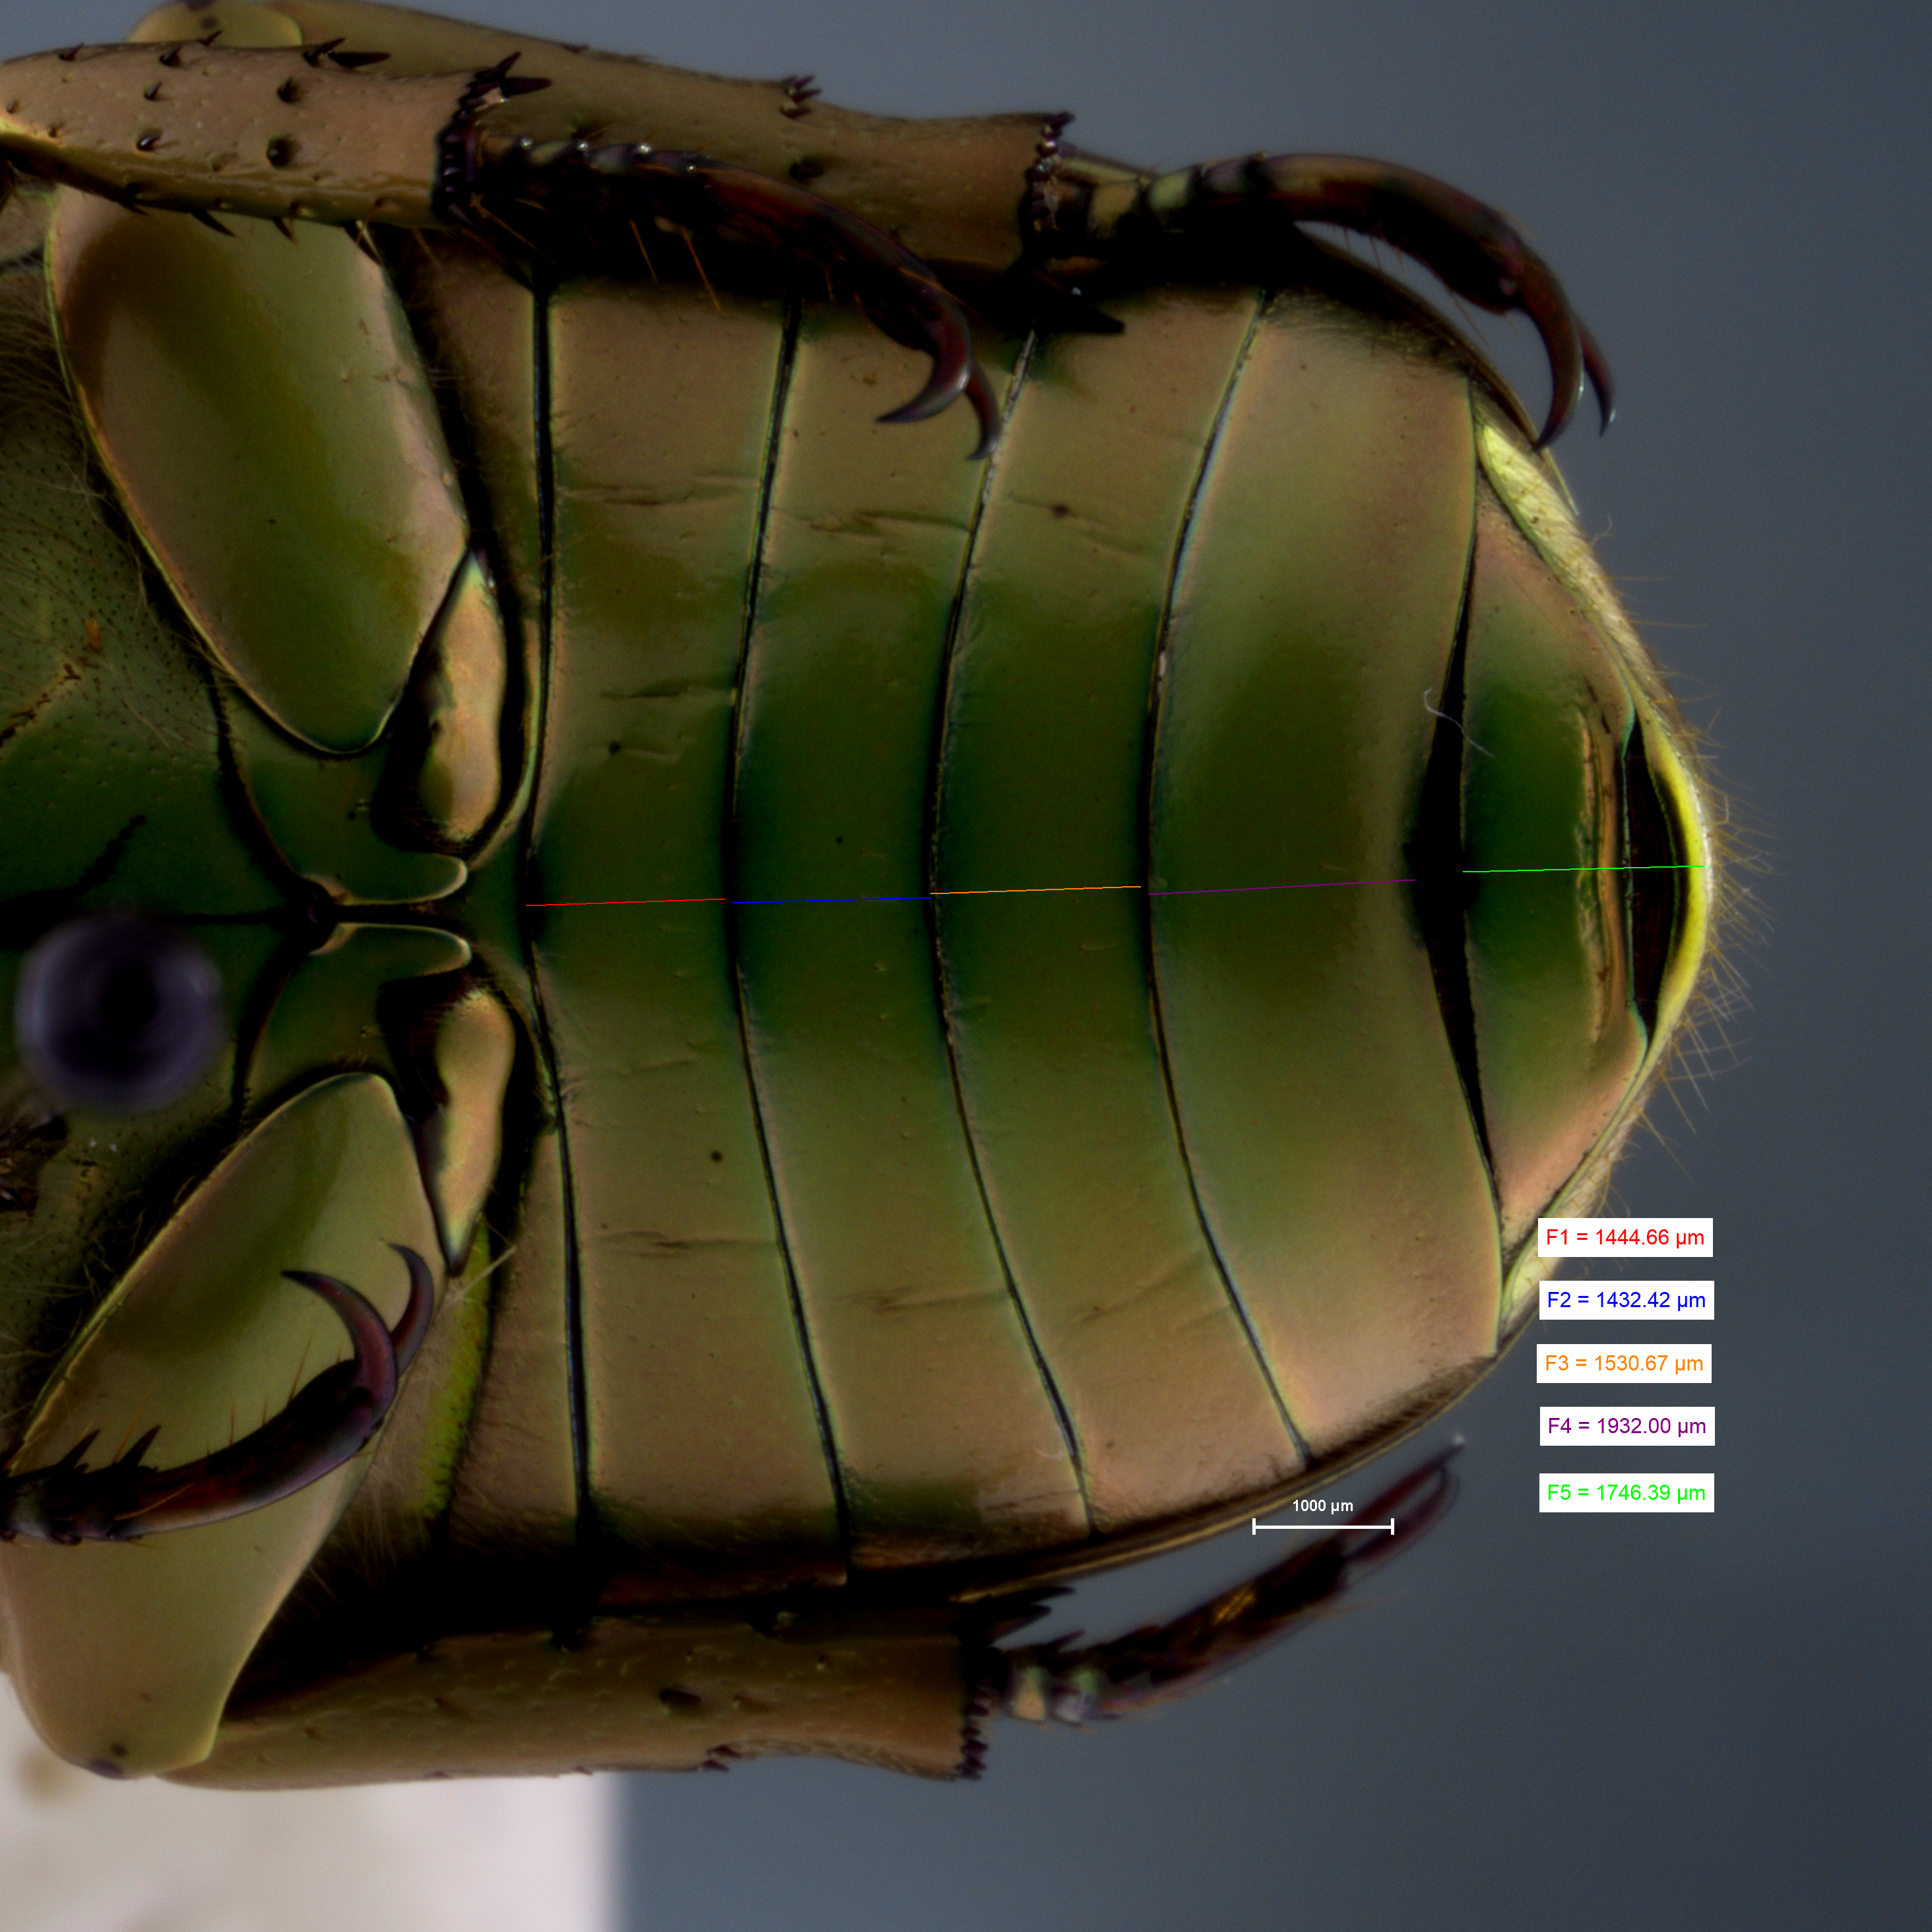
\includegraphics[width=0.5\linewidth]{images/protocol/Ventral.png}
\caption{ Metric F1}
\end{figure}

\newpage
\subsection*{Metric: F2}

Vertical length of the second foremost ventral plate

\begin{figure}[H]
\centering
\includegraphics[width=0.7\linewidth]{images/boxplot/boxplot_F2.png}
\caption{  Boxplot and specimen distribution (superposed) for the metric  F2 by species}
\end{figure}

\noindent\textbf{Test Type:} Student's t-test \\
\noindent\textbf{Test Statistic:} -2.331 \\
\noindent\textbf{P-value:} 0.026 \\
\noindent\textbf{Interpretation:} significant difference

\begin{figure}[H]
\centering
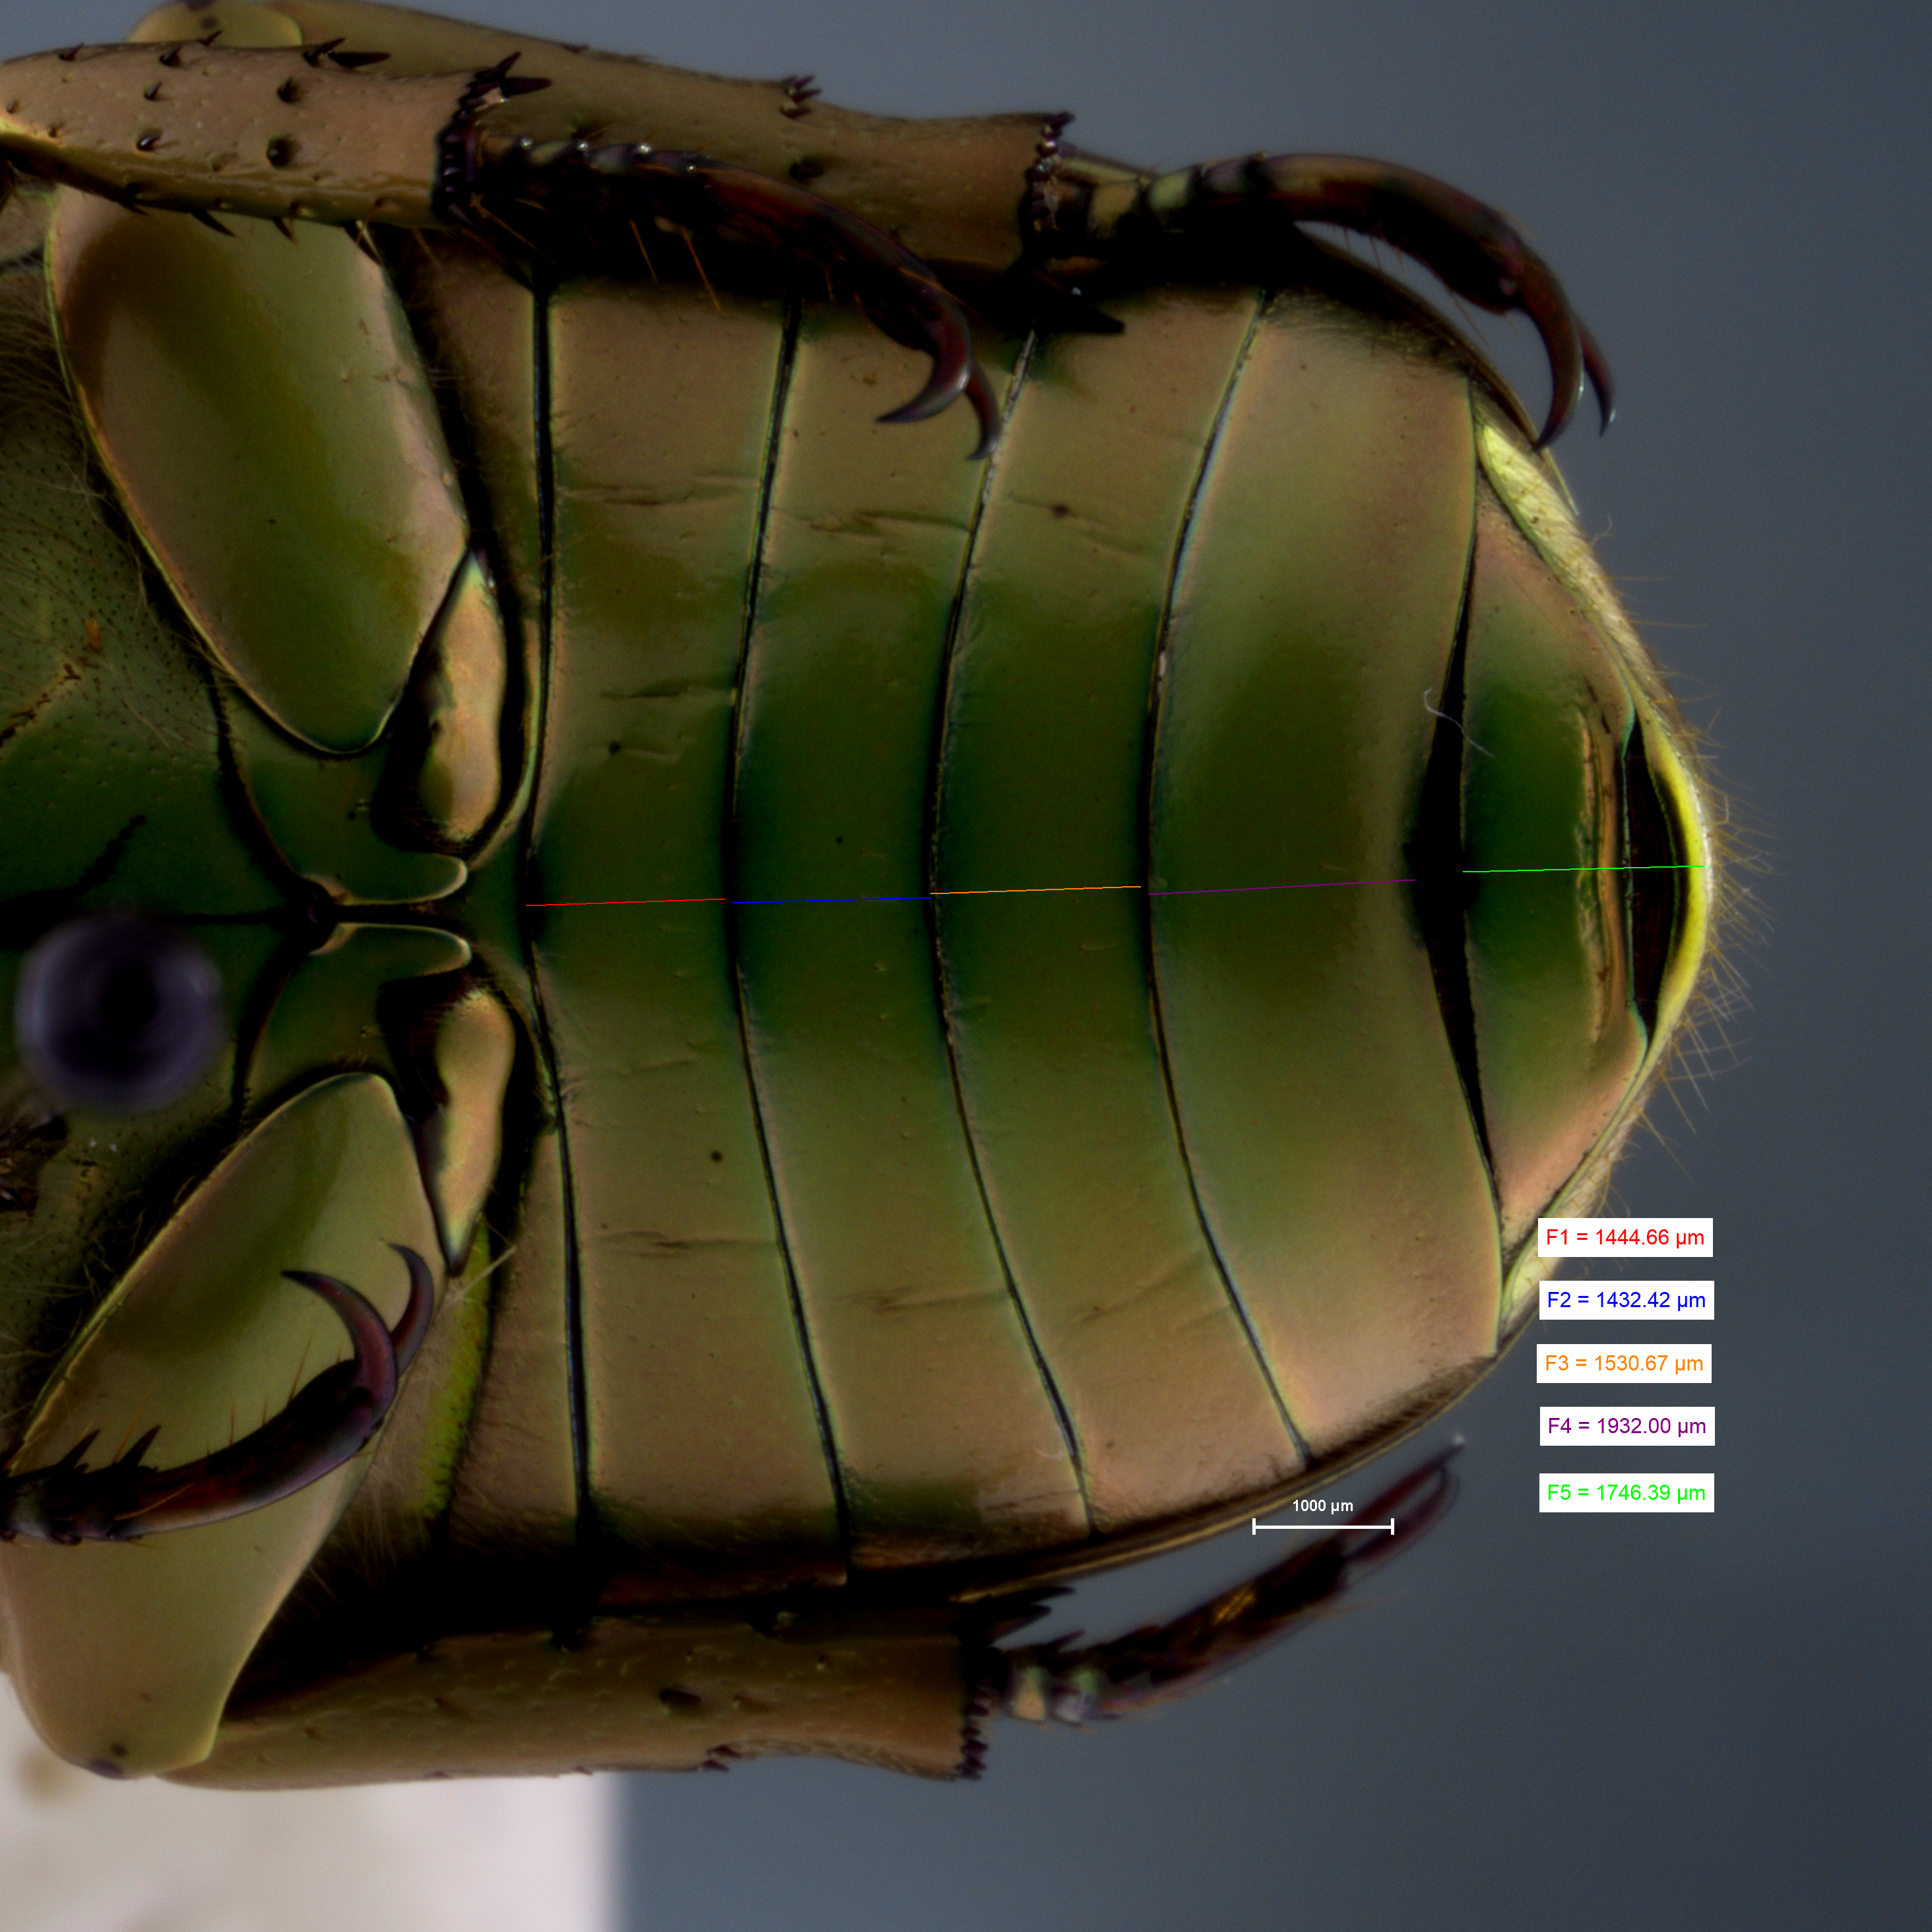
\includegraphics[width=0.5\linewidth]{images/protocol/Ventral.png}
\caption{ Metric F2}
\end{figure}

\newpage
\subsection*{Metric: F3}

Vertical length of the third foremost ventral plate

\begin{figure}[H]
\centering
\includegraphics[width=0.7\linewidth]{images/boxplot/boxplot_F3.png}
\caption{  Boxplot and specimen distribution (superposed) for the metric  F3 by species}
\end{figure}

\noindent\textbf{Test Type:} Student's t-test \\
\noindent\textbf{Test Statistic:} -2.605 \\
\noindent\textbf{P-value:} 0.014 \\
\noindent\textbf{Interpretation:} significant difference

\begin{figure}[H]
\centering
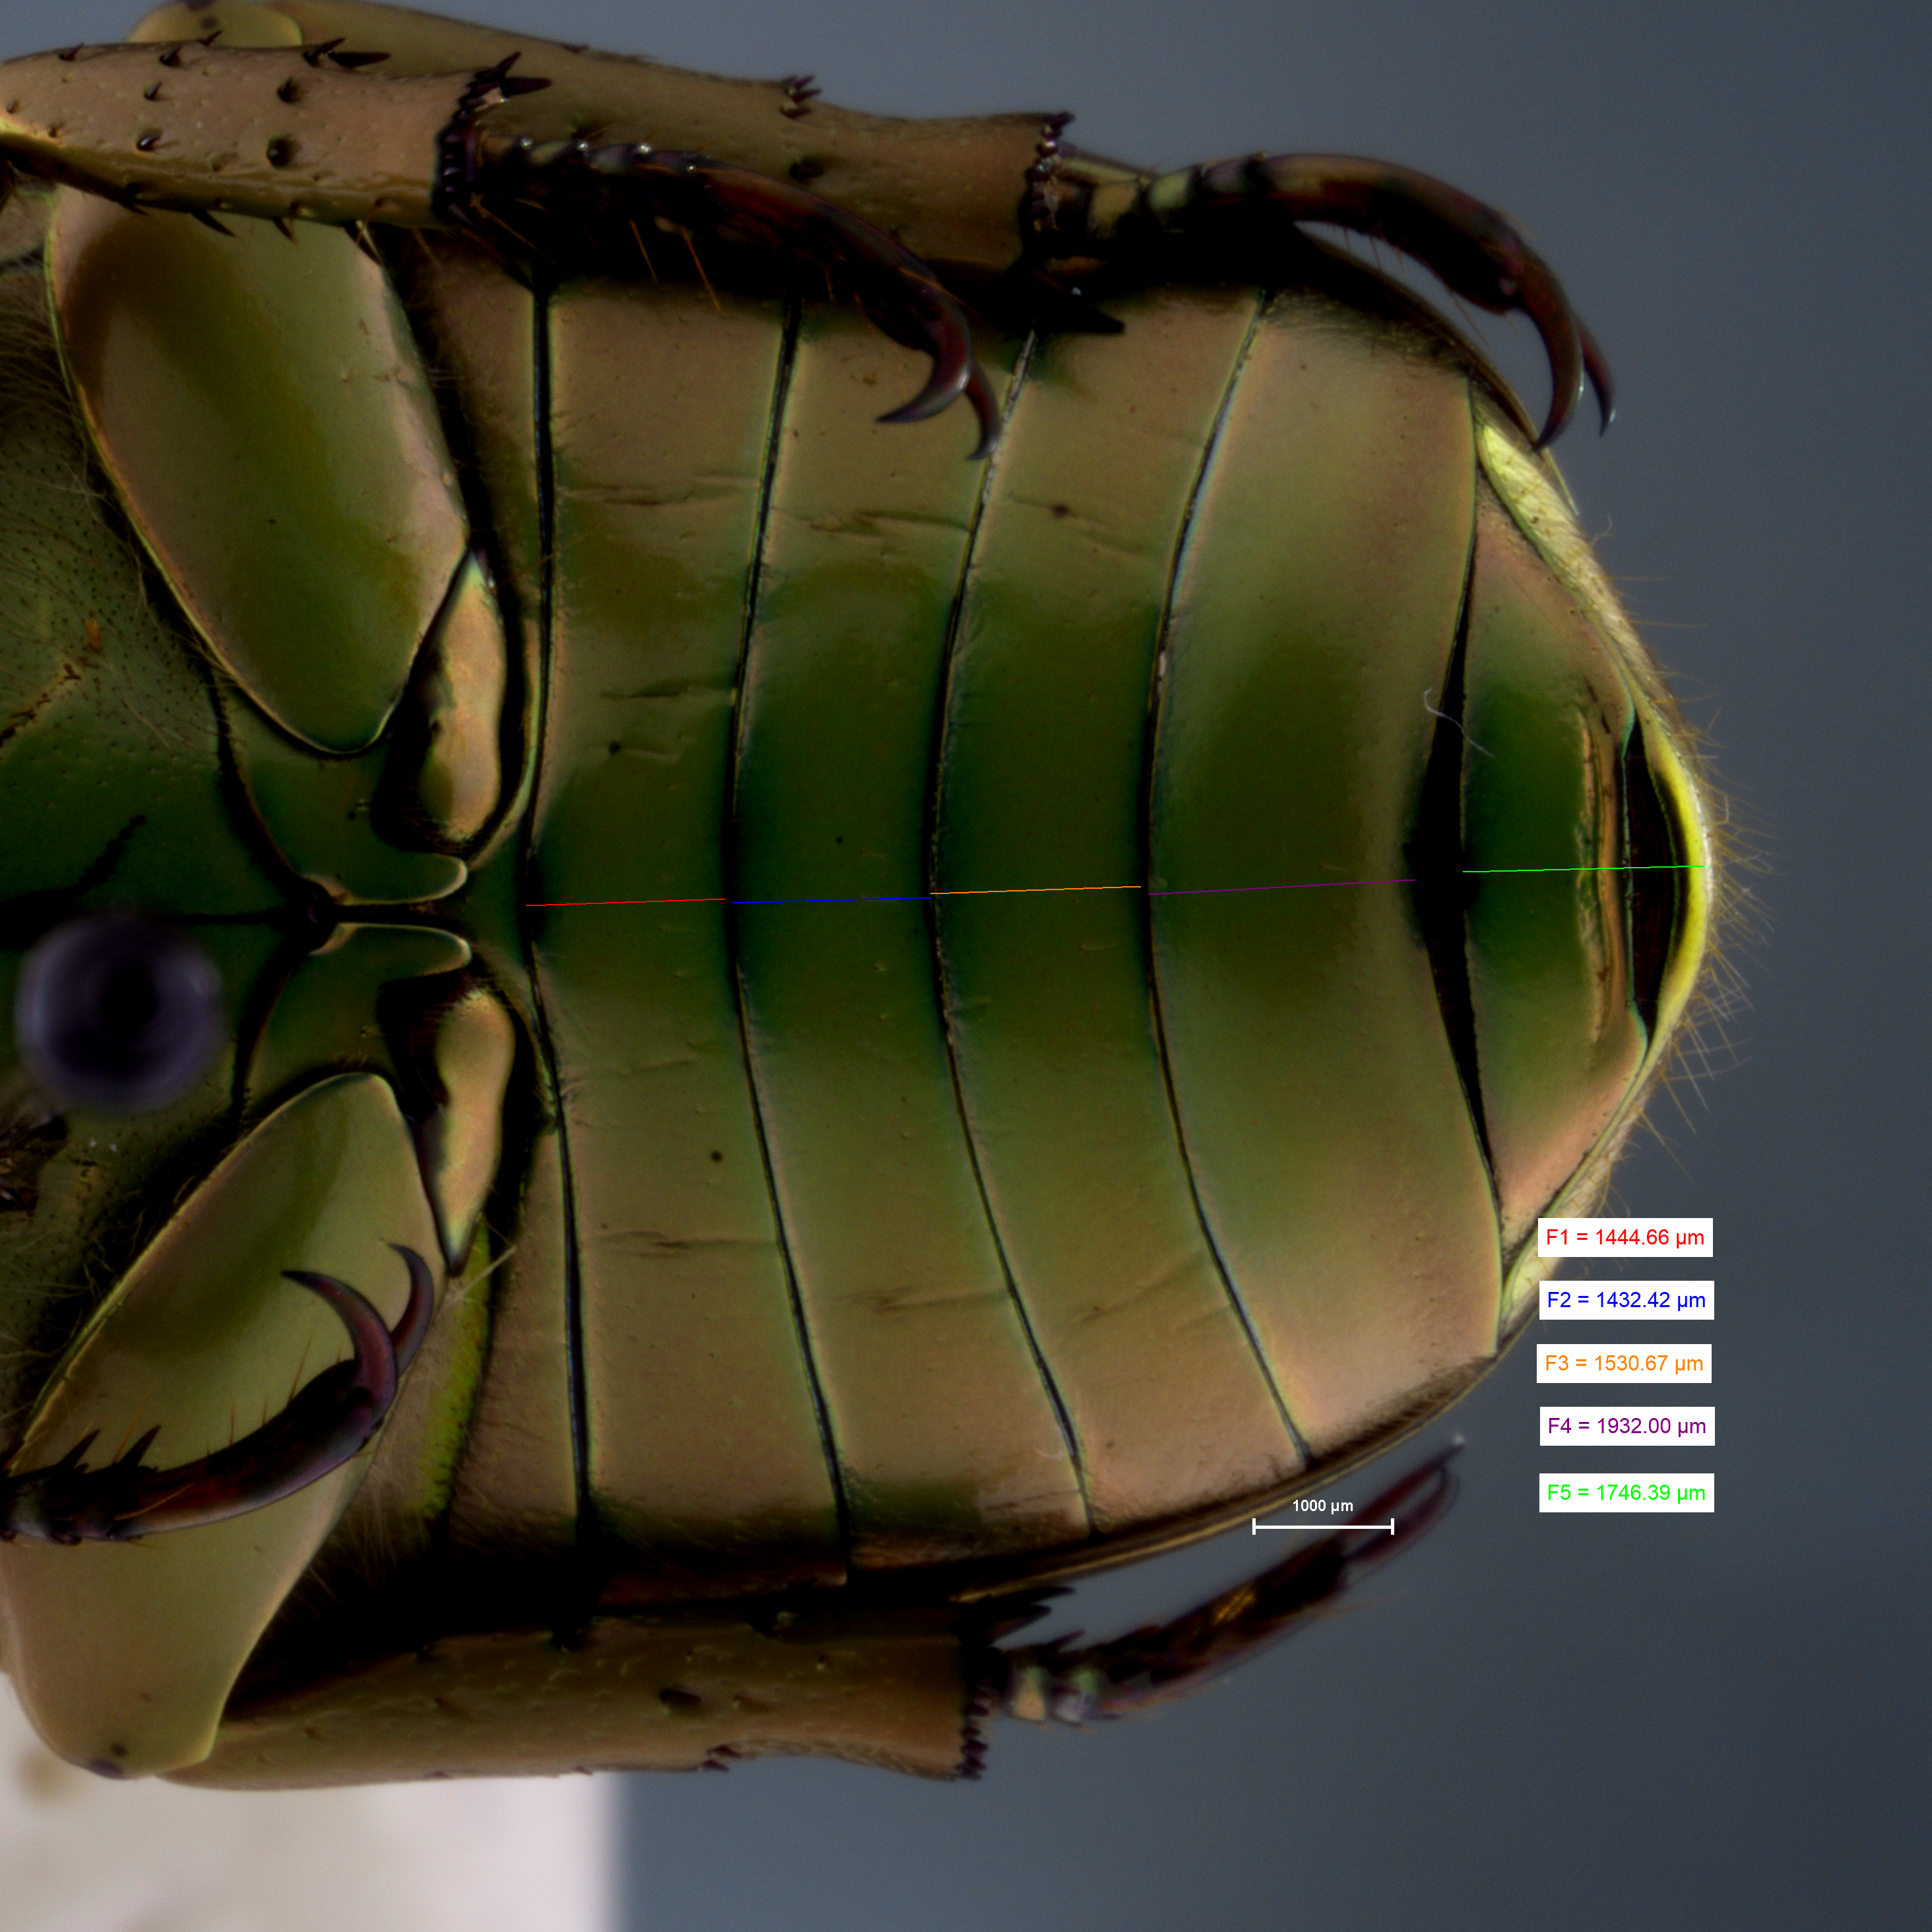
\includegraphics[width=0.5\linewidth]{images/protocol/Ventral.png}
\caption{ Metric F3}
\end{figure}

\newpage
\subsection*{Metric: F4}

Vertical length of the fourth foremost ventral plate 

\begin{figure}[H]
\centering
\includegraphics[width=0.7\linewidth]{images/boxplot/boxplot_F4.png}
\caption{  Boxplot and specimen distribution (superposed) for the metric  F4 by species}
\end{figure}

\noindent\textbf{Test Type:} Student's t-test \\
\noindent\textbf{Test Statistic:} -2.925 \\
\noindent\textbf{P-value:} 0.006 \\
\noindent\textbf{Interpretation:} significant difference

\begin{figure}[H]
\centering
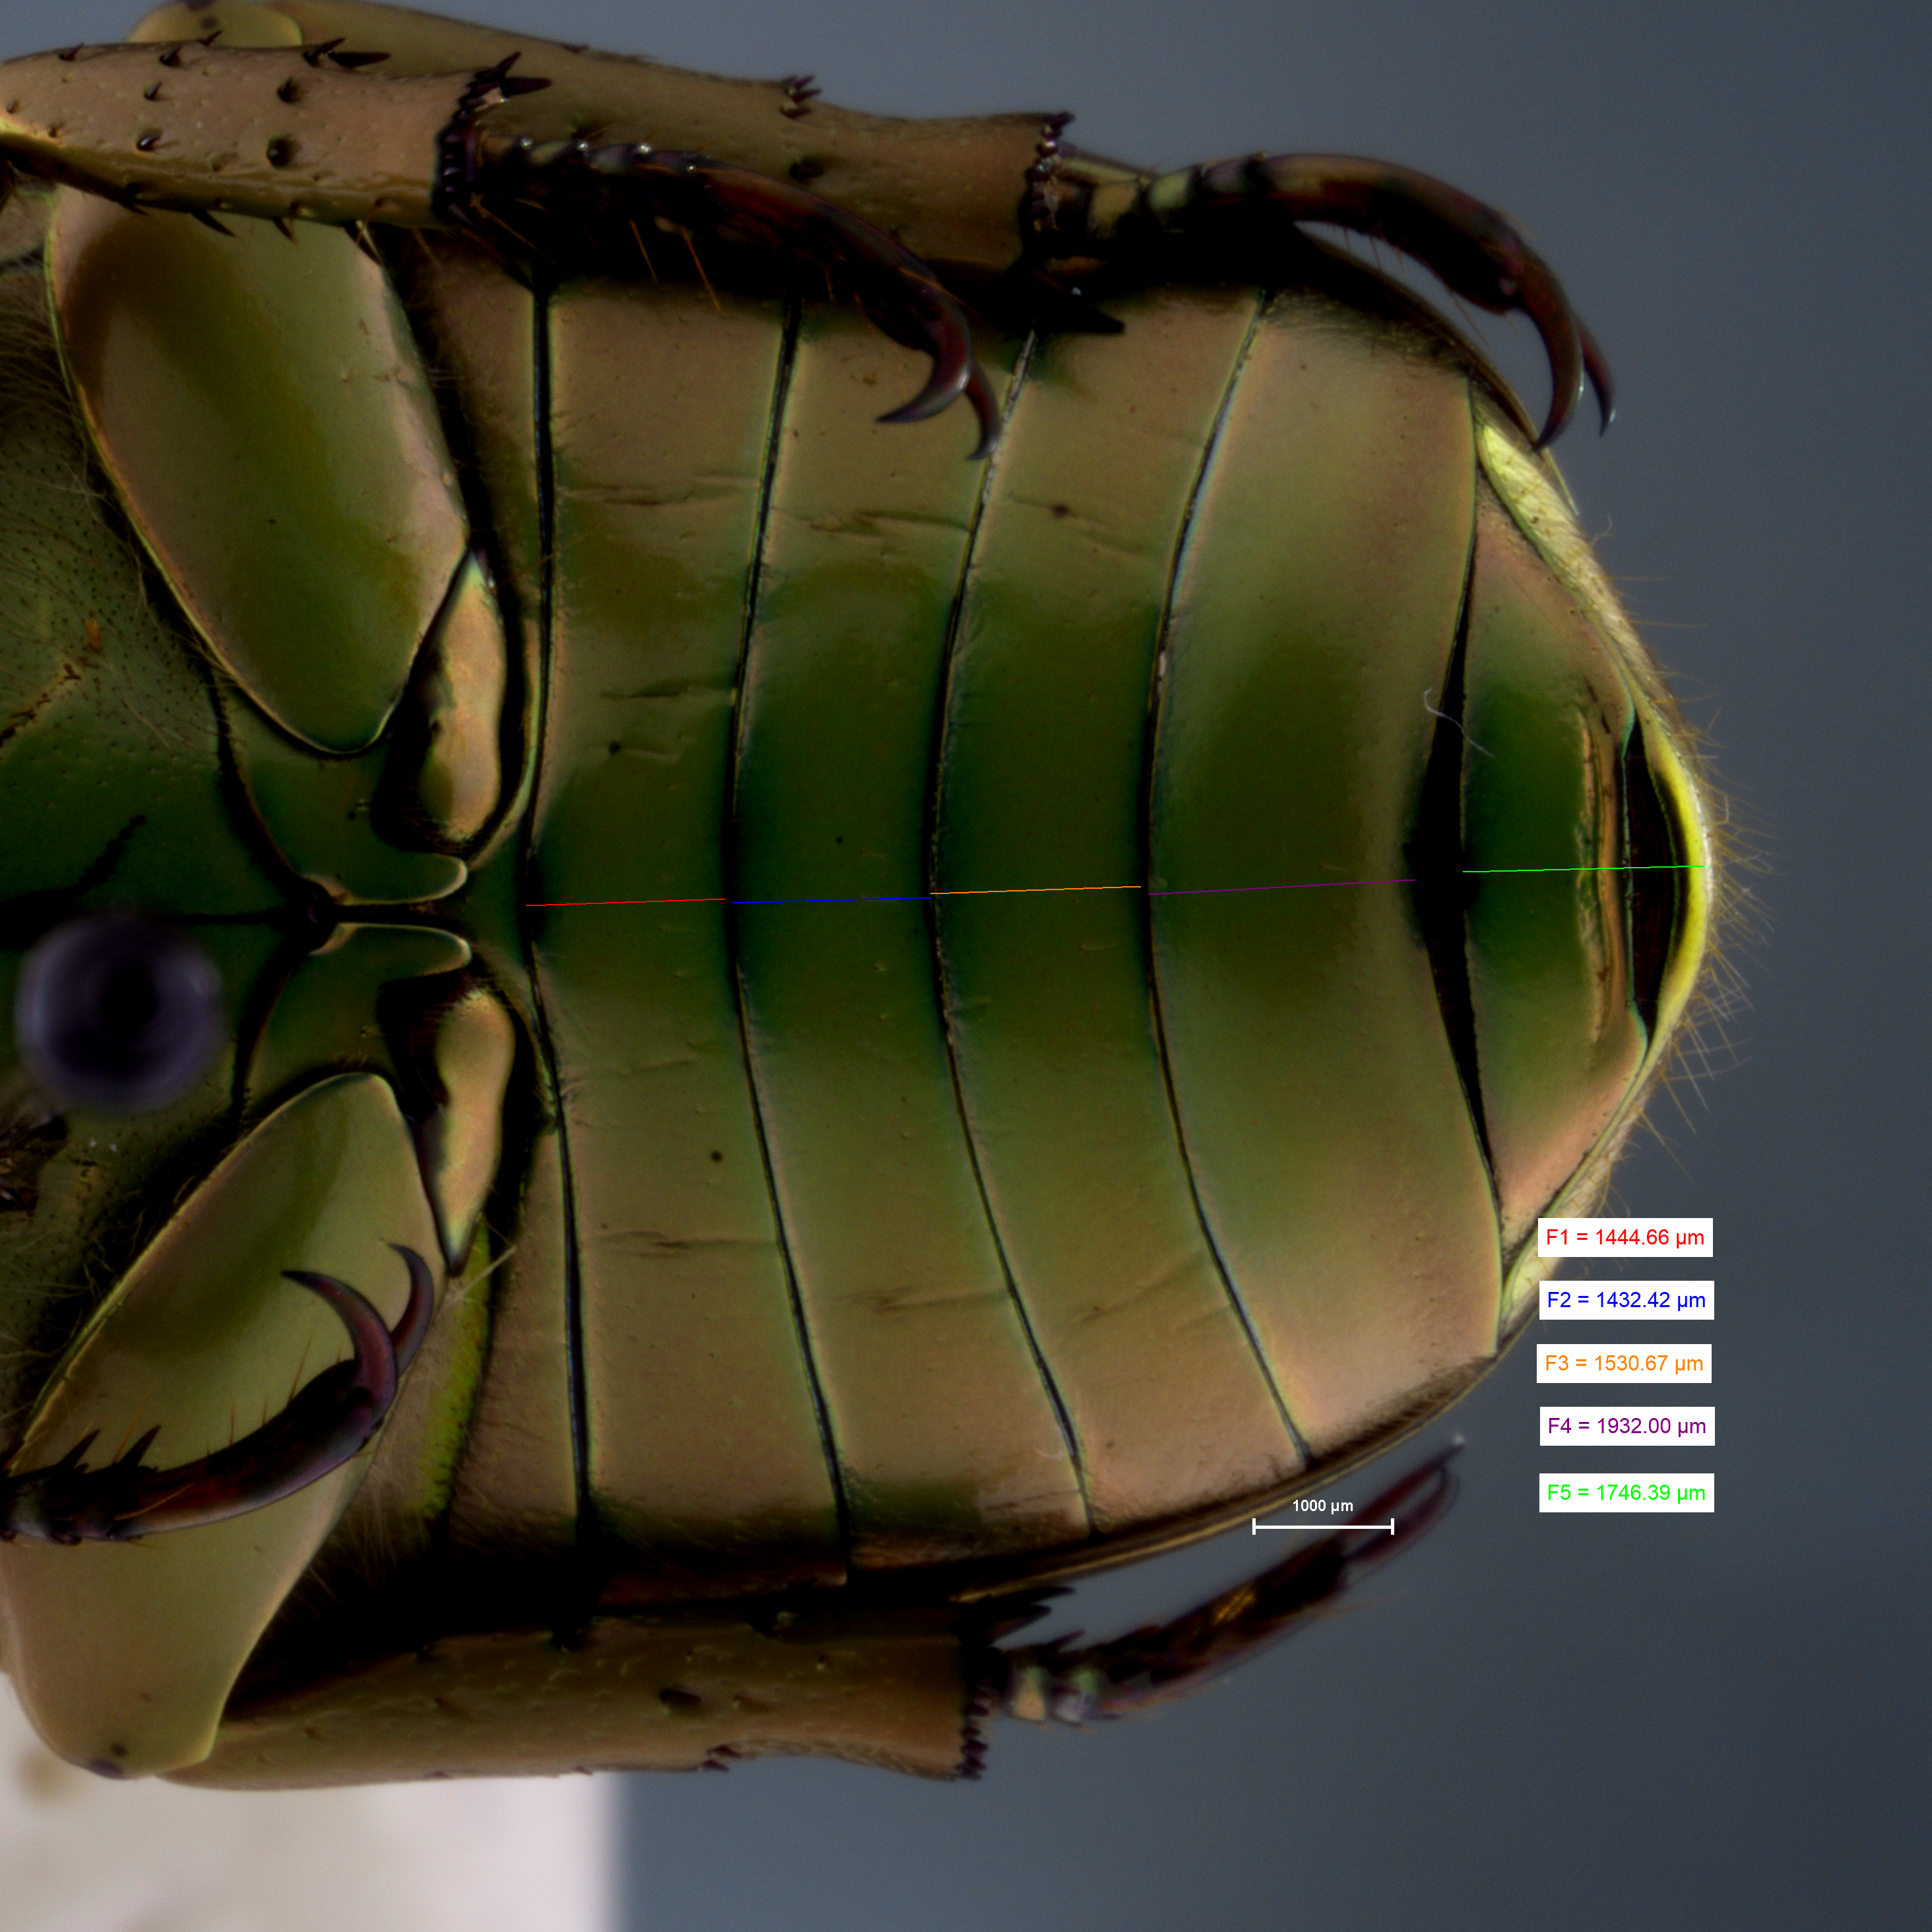
\includegraphics[width=0.5\linewidth]{images/protocol/Ventral.png}
\caption{ Metric F4}
\end{figure}

\newpage
\subsection*{Metric: F5}

Vertical length of the fifth foremost ventral plate

\begin{figure}[H]
\centering
\includegraphics[width=0.7\linewidth]{images/boxplot/boxplot_F5.png}
\caption{  Boxplot and specimen distribution (superposed) for the metric  F5 by species}
\end{figure}

\noindent\textbf{Test Type:} Student's t-test \\
\noindent\textbf{Test Statistic:} -1.949 \\
\noindent\textbf{P-value:} 0.060 \\
\noindent\textbf{Interpretation:} no significant difference

\begin{figure}[H]
\centering
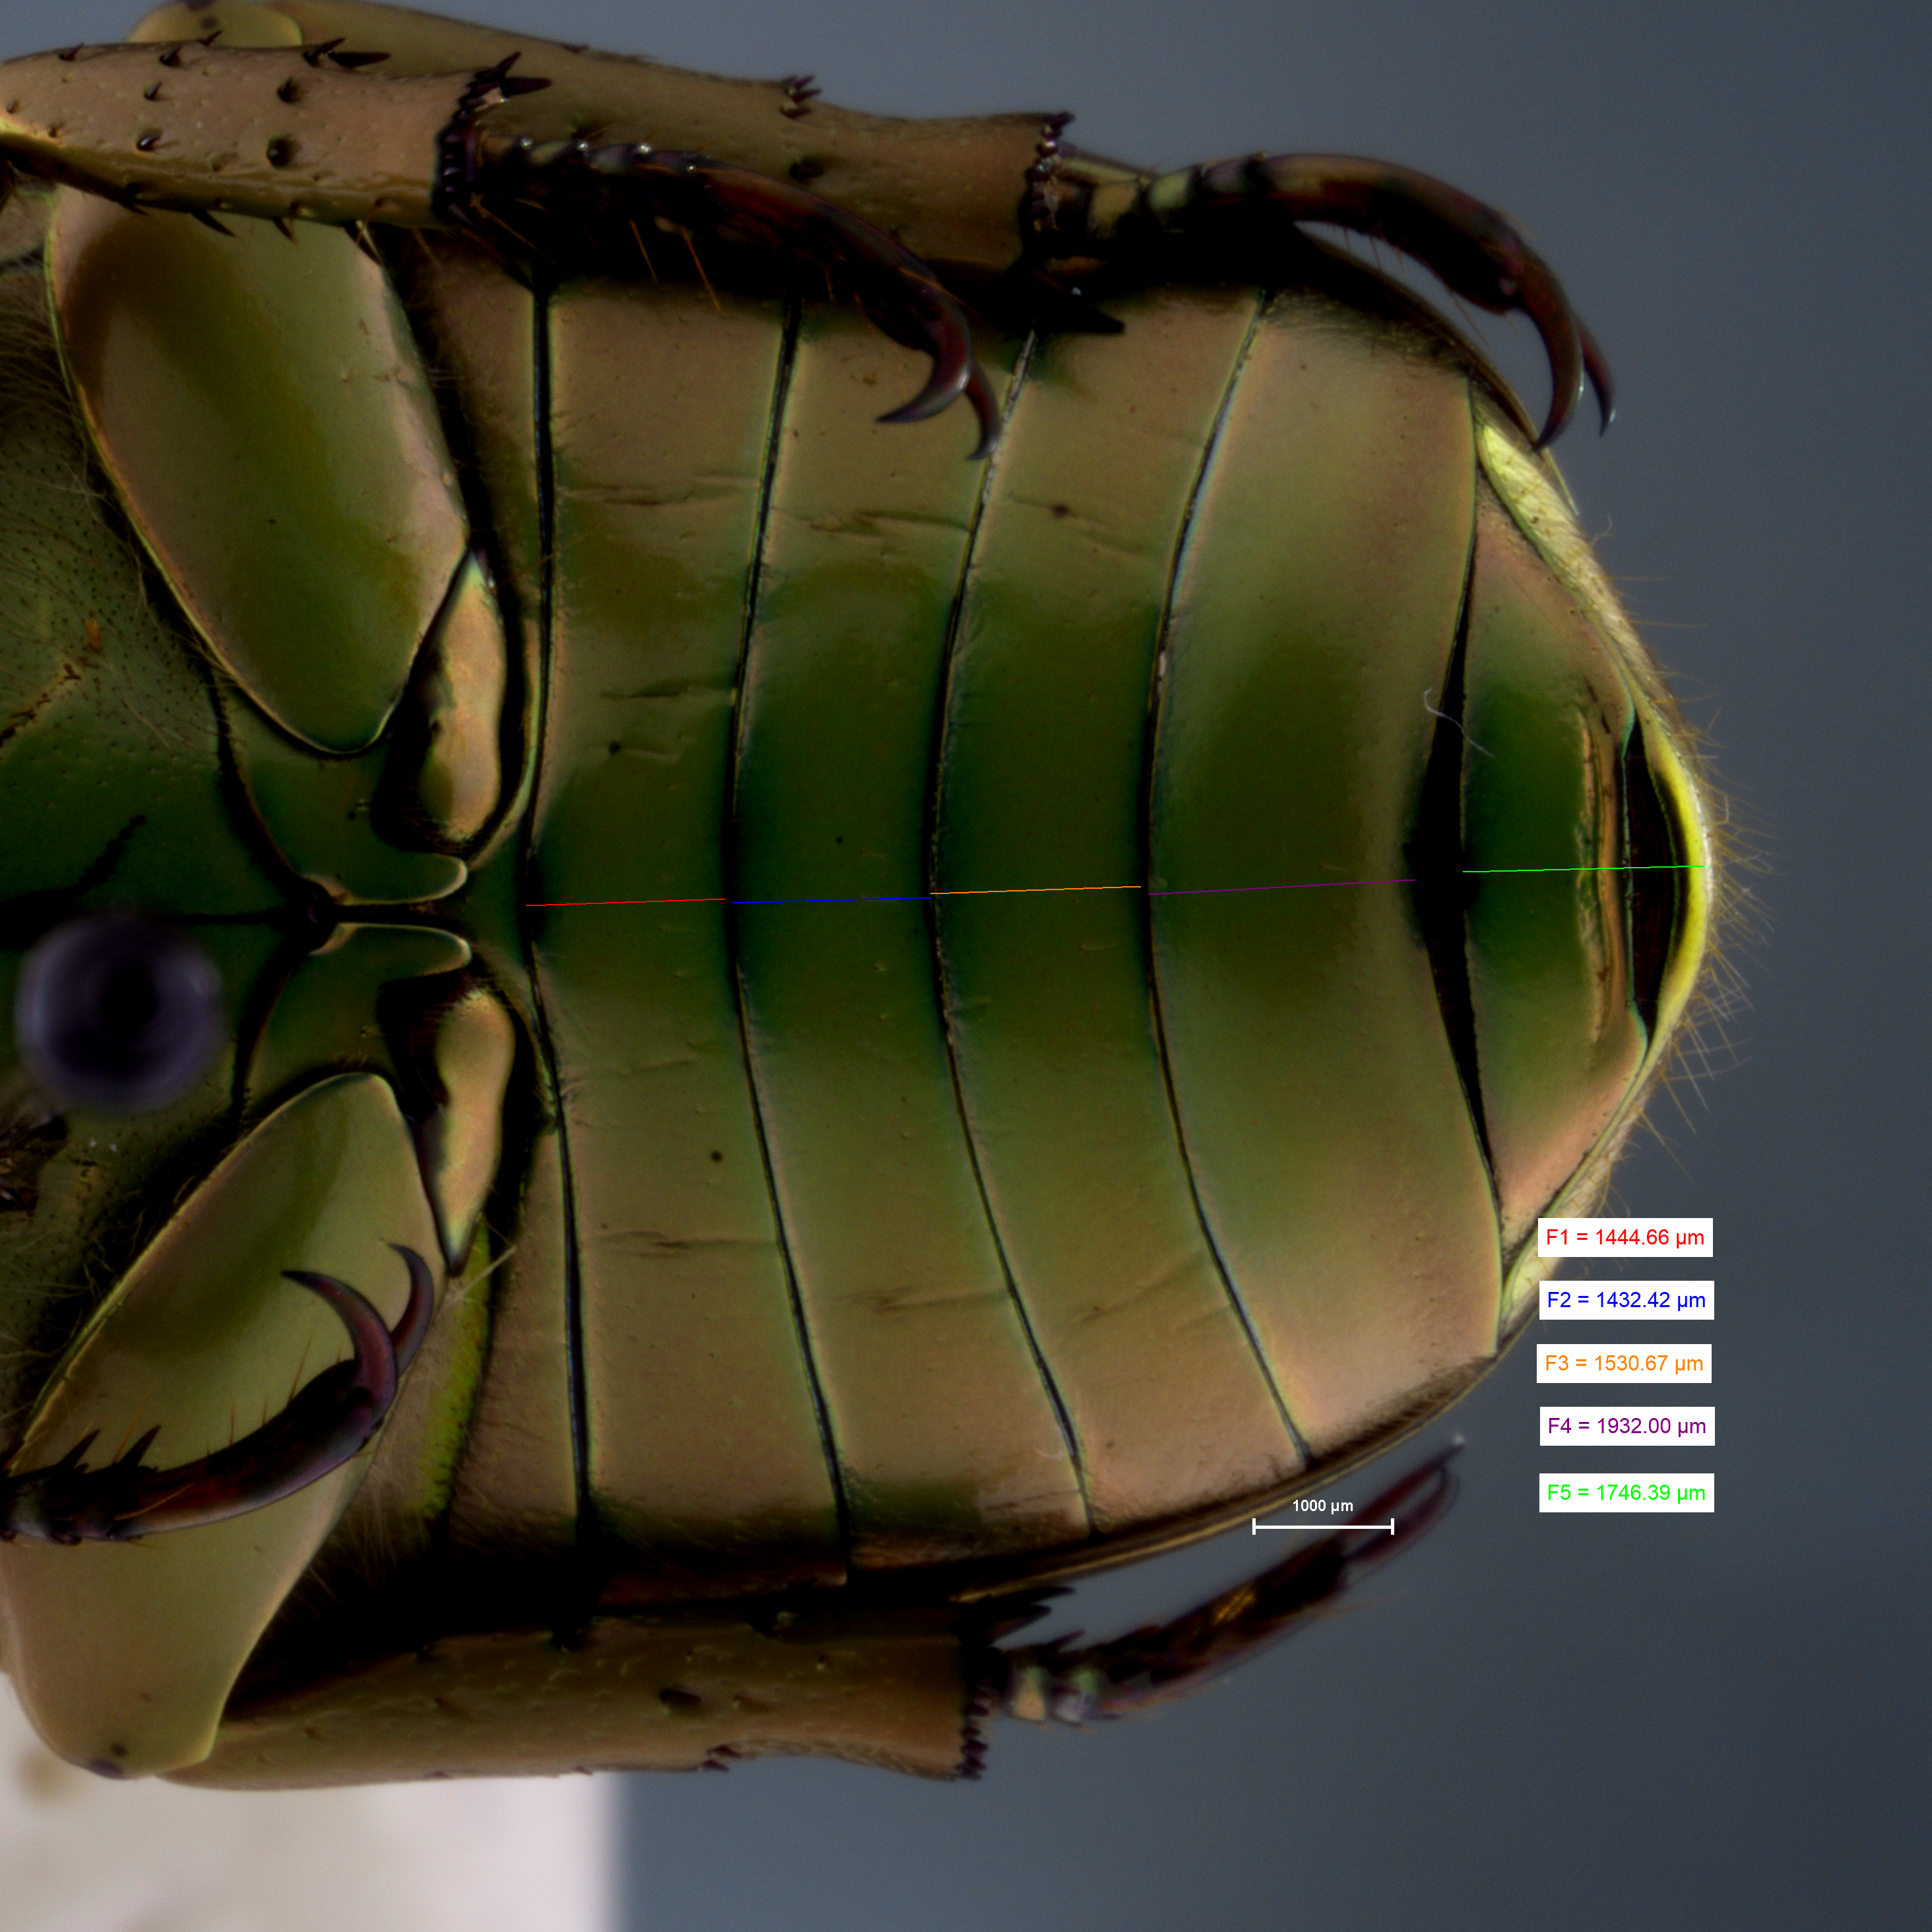
\includegraphics[width=0.5\linewidth]{images/protocol/Ventral.png}
\caption{ Metric F5}
\end{figure}

\newpage
\subsection*{Metric: A1÷A3}

A1/A3 Measure of the vertical length of beetle's head relative to its canthuses' distance width

\begin{figure}[H]
\centering
\includegraphics[width=0.7\linewidth]{images/boxplot/boxplot_A1÷A3.png}
\caption{  Boxplot and specimen distribution (superposed) for the metric  A1÷A3 by species}
\end{figure}

\noindent\textbf{Test Type:} Student's t-test \\
\noindent\textbf{Test Statistic:} 0.140 \\
\noindent\textbf{P-value:} 0.890 \\
\noindent\textbf{Interpretation:} no significant difference

\begin{figure}[H]
\centering
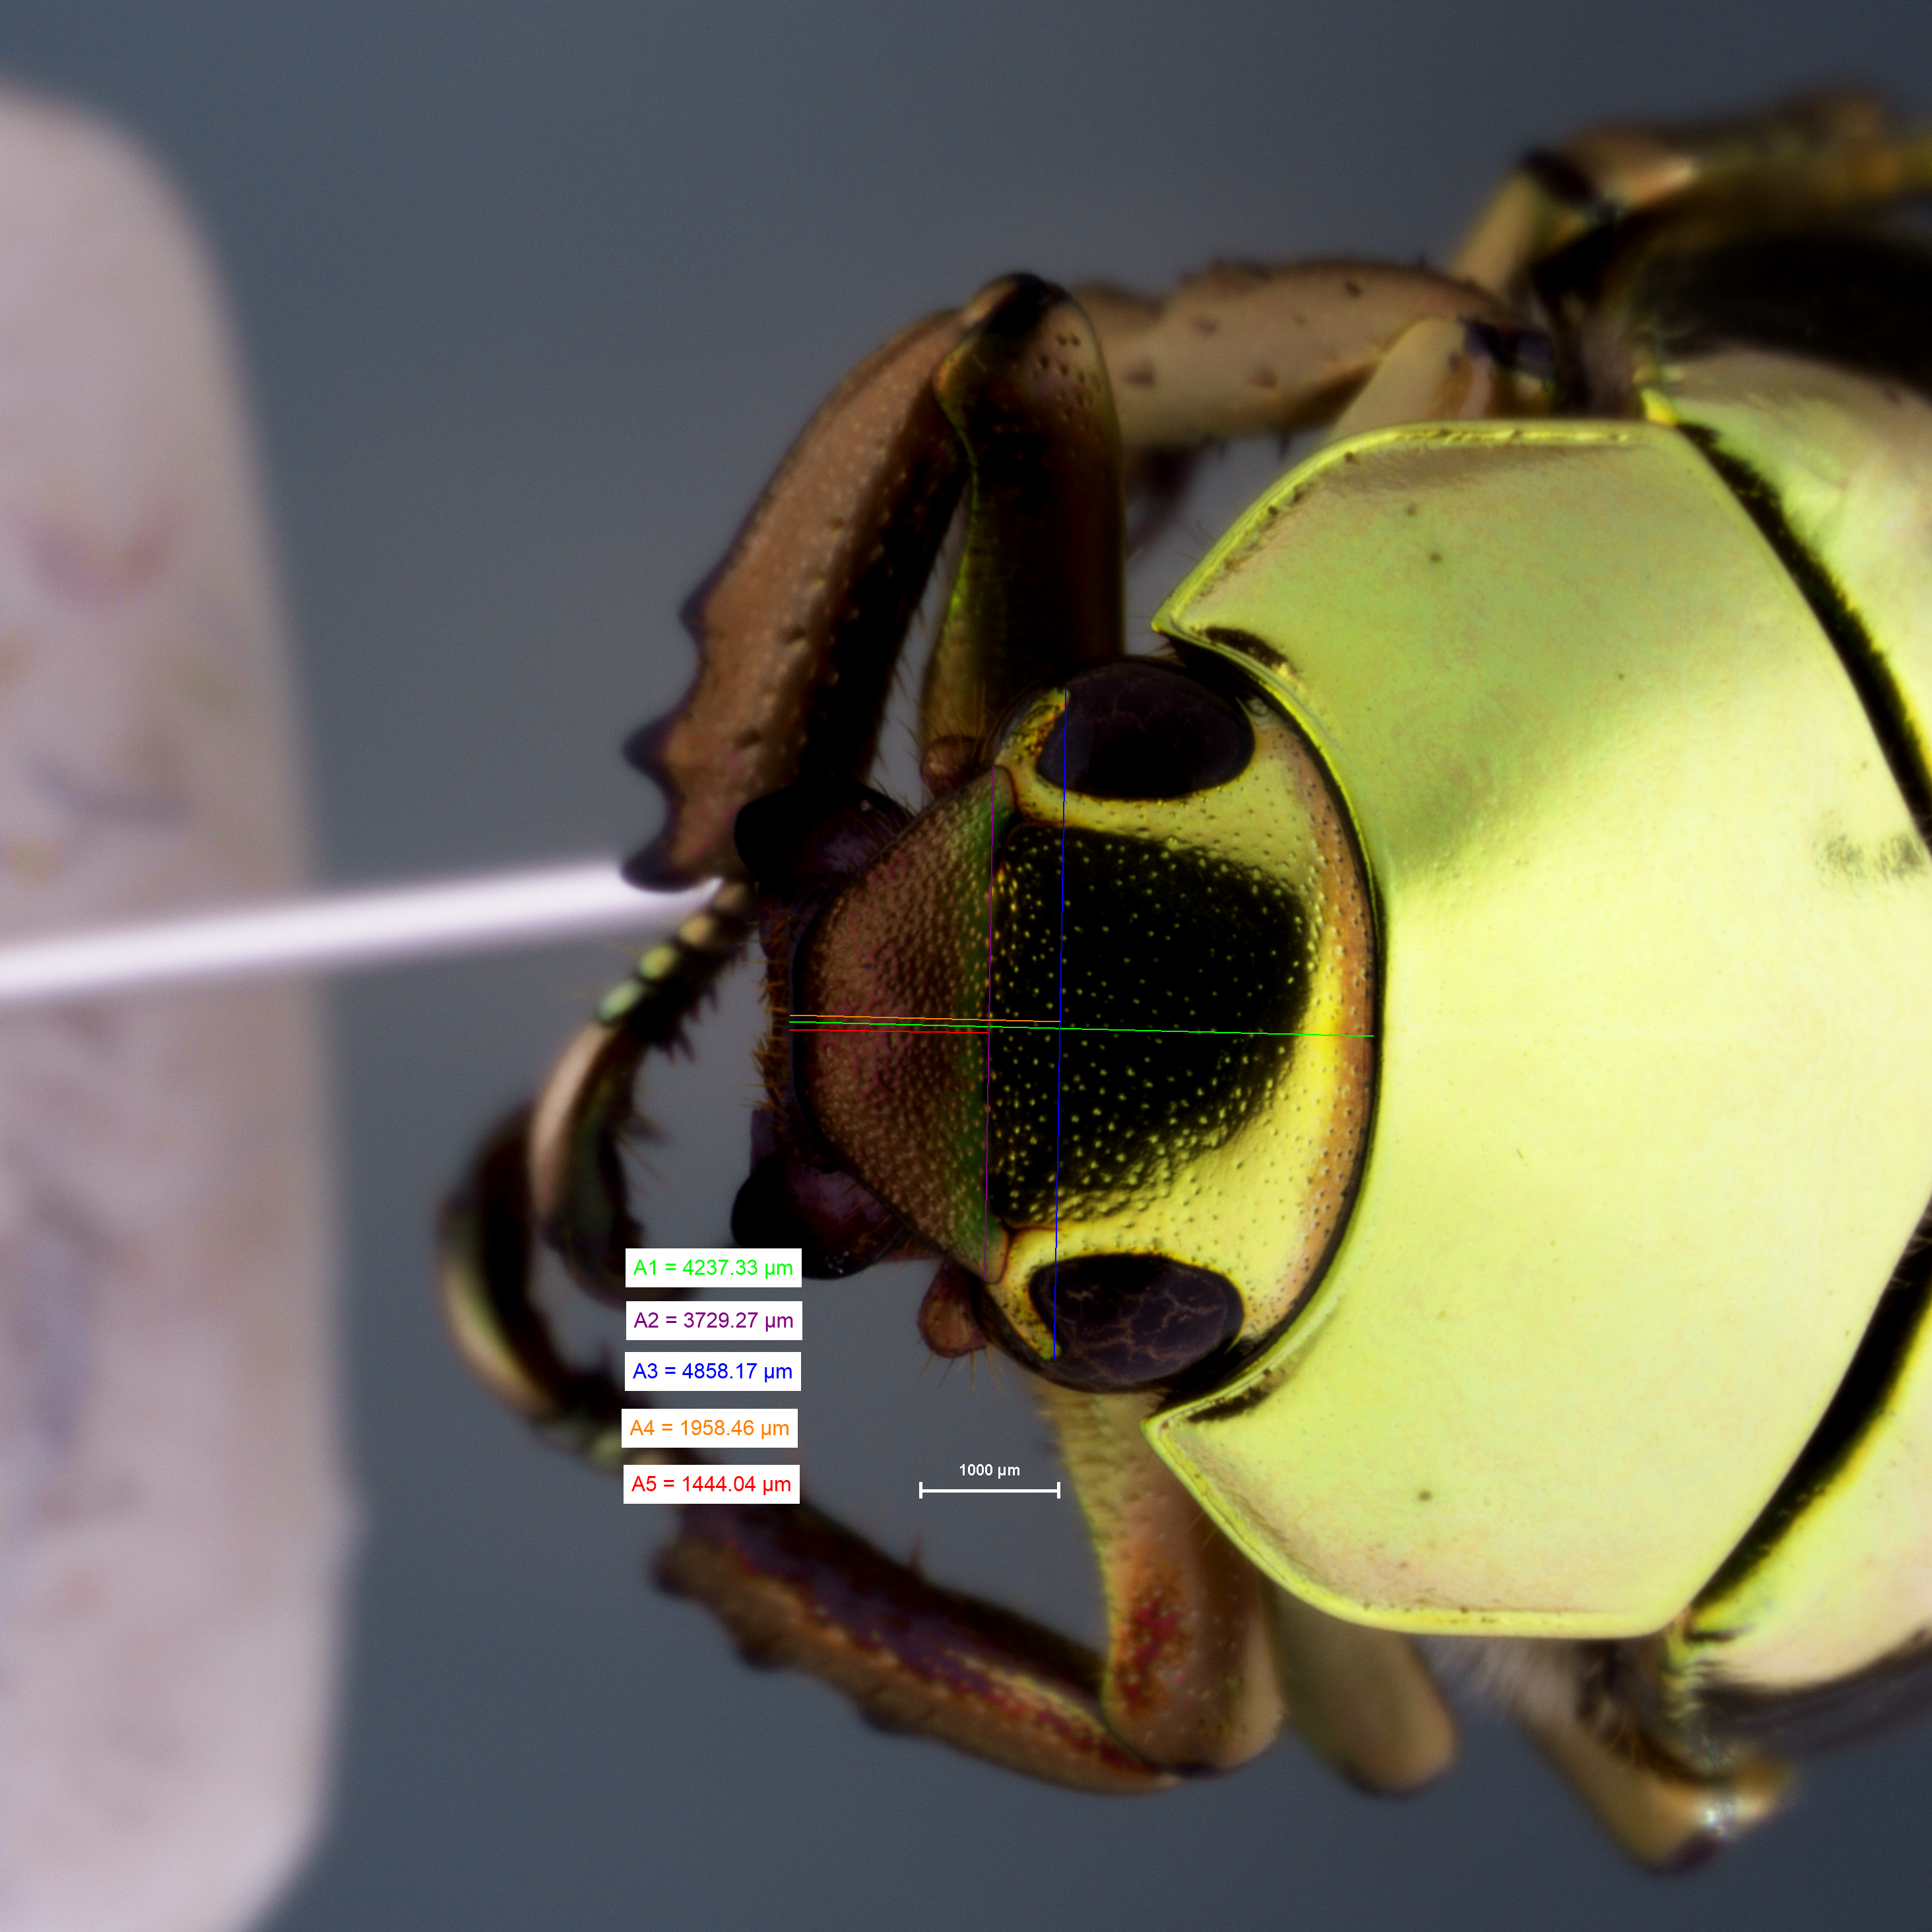
\includegraphics[width=0.5\linewidth]{images/protocol/Head.png}
\caption{ Metric A1÷A3}
\end{figure}

\newpage
\subsection*{Metric: A4÷A3}

A4/A3 Measure of the vertical length of beetle's clipeum relative to its canthuses' distance width

\begin{figure}[H]
\centering
\includegraphics[width=0.7\linewidth]{images/boxplot/boxplot_A4÷A3.png}
\caption{  Boxplot and specimen distribution (superposed) for the metric  A4÷A3 by species}
\end{figure}

\noindent\textbf{Test Type:} Mann-Whitney U test \\
\noindent\textbf{Test Statistic:} 56.000 \\
\noindent\textbf{P-value:} 0.511 \\
\noindent\textbf{Interpretation:} no significant difference

\begin{figure}[H]
\centering
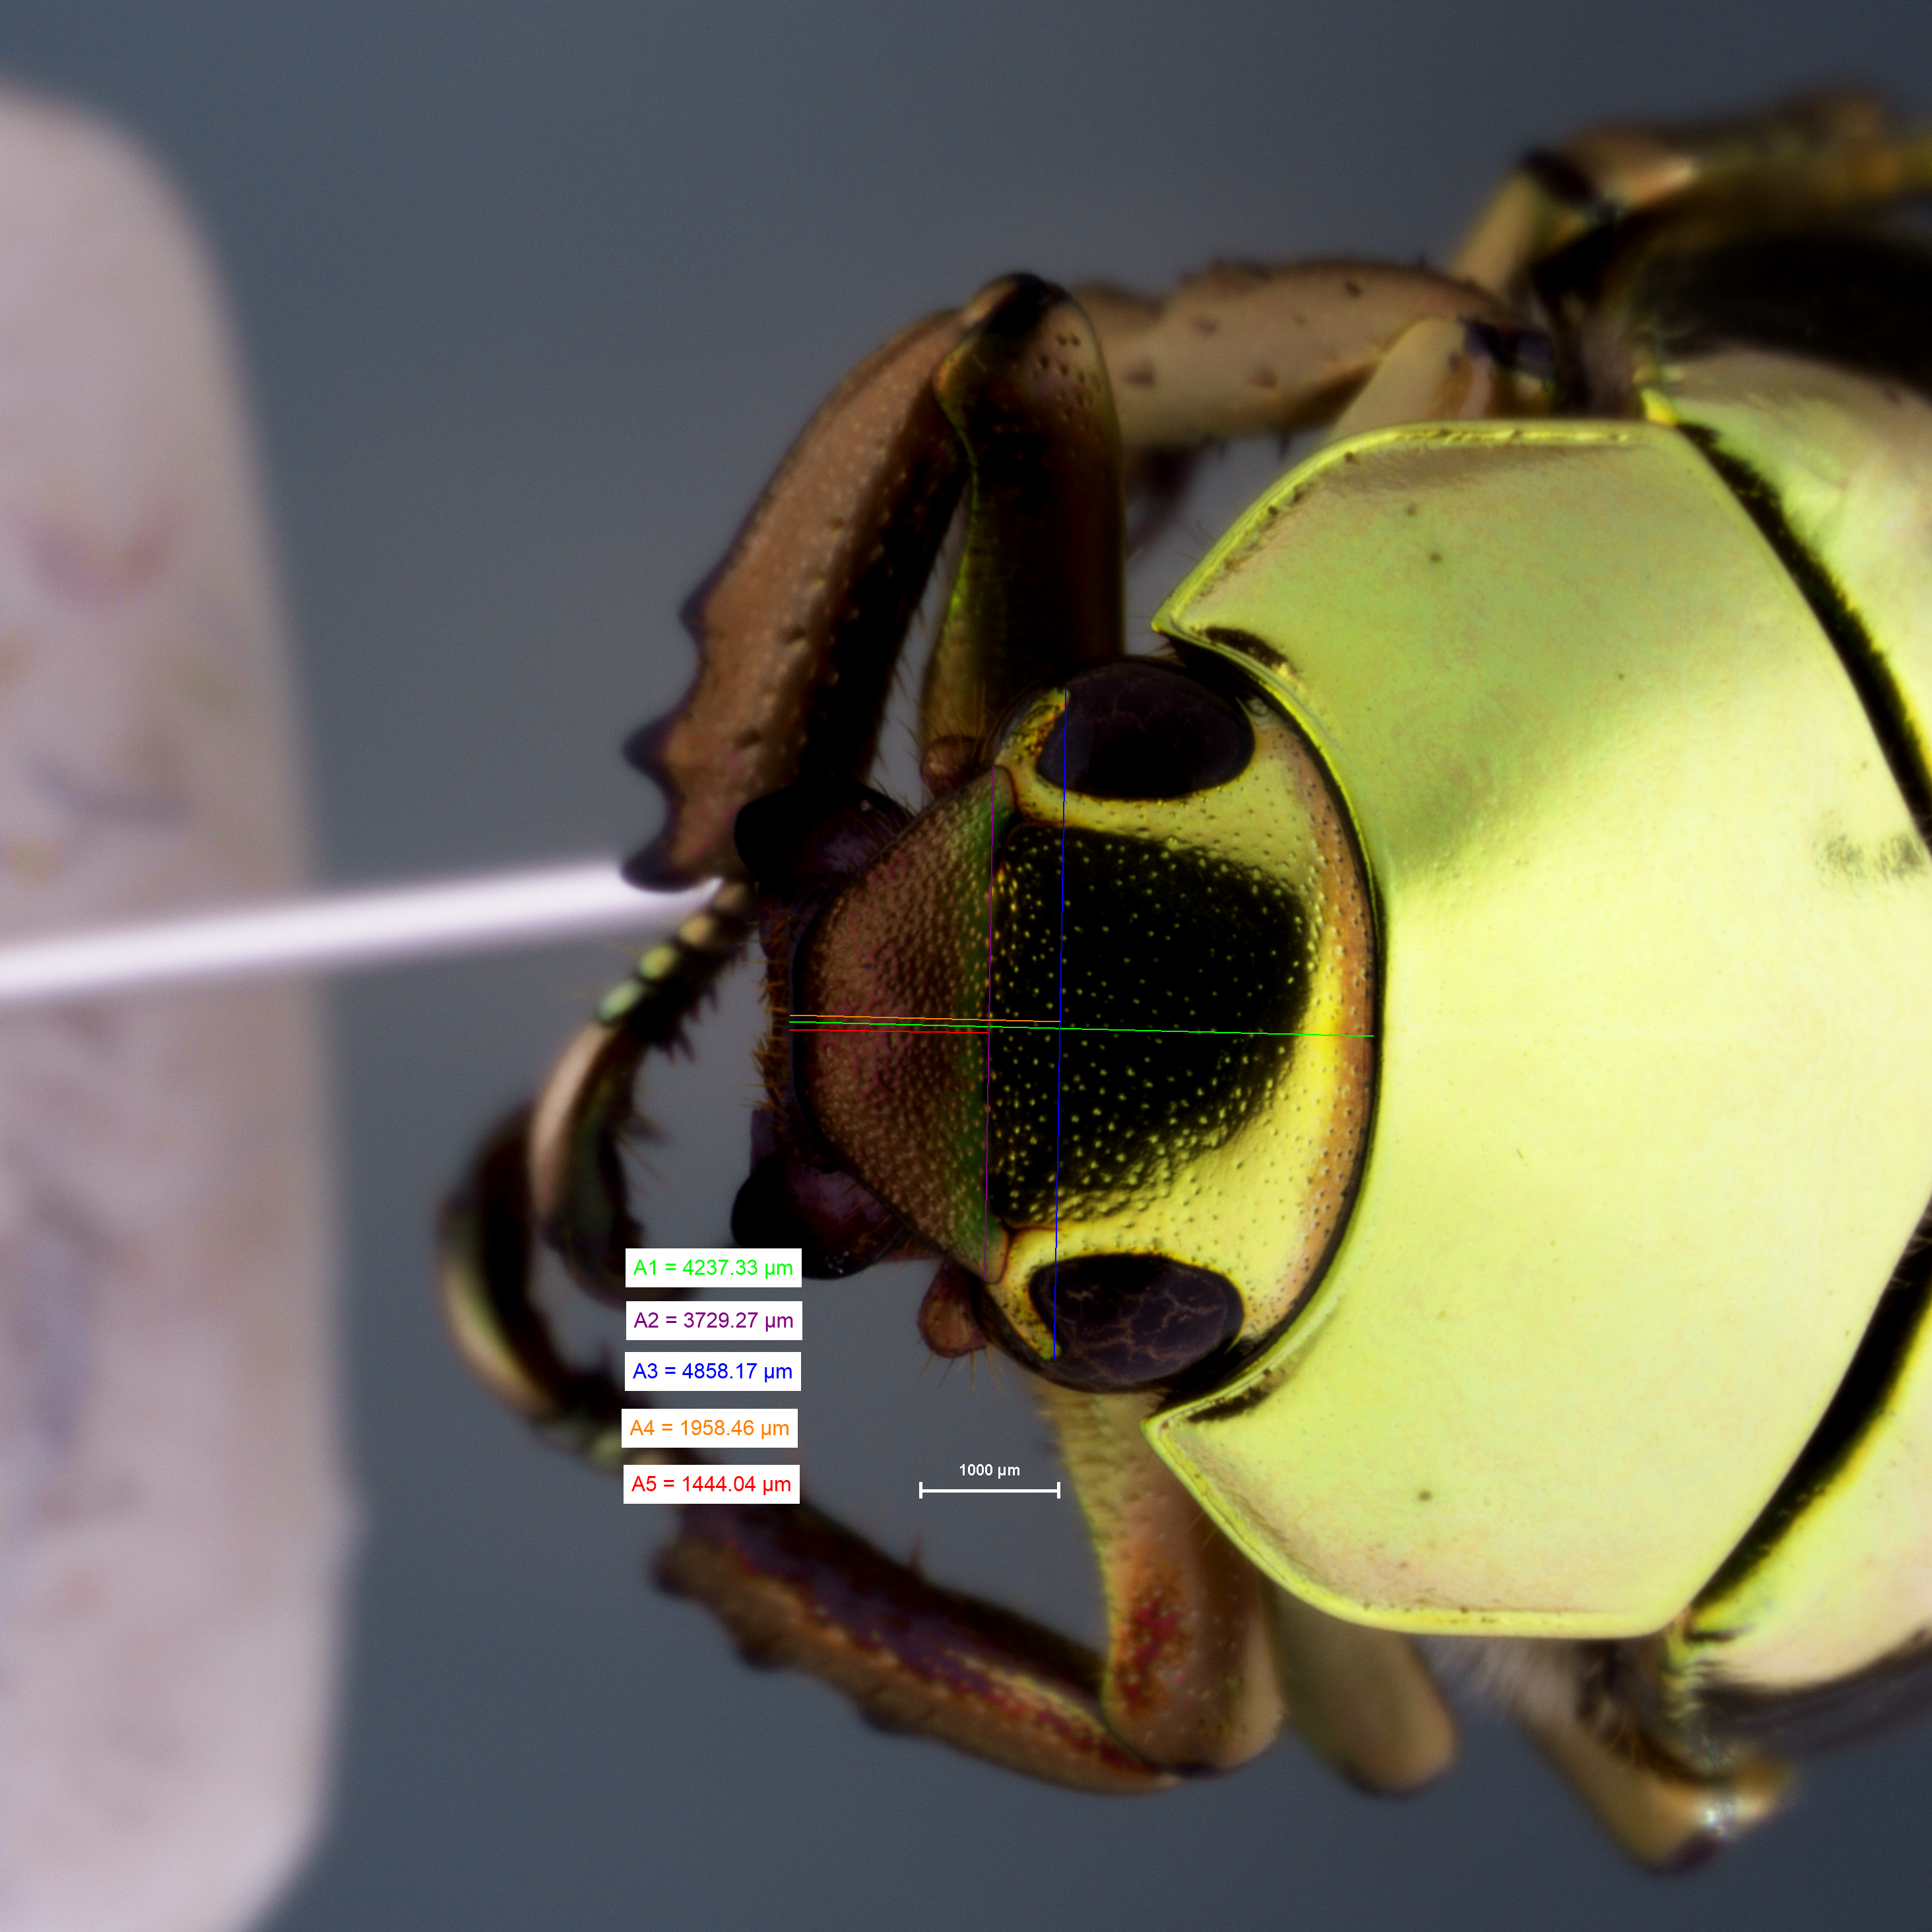
\includegraphics[width=0.5\linewidth]{images/protocol/Head.png}
\caption{ Metric A4÷A3}
\end{figure}

\newpage
\subsection*{Metric: A5÷A3}

A5/A3 Measure of the vertical length of beetle's eyes relative to its canthuses' distance width

\begin{figure}[H]
\centering
\includegraphics[width=0.7\linewidth]{images/boxplot/boxplot_A5÷A3.png}
\caption{  Boxplot and specimen distribution (superposed) for the metric  A5÷A3 by species}
\end{figure}

\noindent\textbf{Test Type:} Mann-Whitney U test \\
\noindent\textbf{Test Statistic:} 77.000 \\
\noindent\textbf{P-value:} 0.694 \\
\noindent\textbf{Interpretation:} no significant difference

\begin{figure}[H]
\centering
\includegraphics[width=0.5\linewidth]{images/protocol/Head.png}
\caption{ Metric A5÷A3}
\end{figure}

\newpage
\subsection*{Metric: B4÷B1}

Measure of the vertical length of the pronotum relative to its front width. B4/B1

\begin{figure}[H]
\centering
\includegraphics[width=0.7\linewidth]{images/boxplot/boxplot_B4÷B1.png}
\caption{  Boxplot and specimen distribution (superposed) for the metric  B4÷B1 by species}
\end{figure}

\noindent\textbf{Test Type:} Mann-Whitney U test \\
\noindent\textbf{Test Statistic:} 142.000 \\
\noindent\textbf{P-value:} 0.581 \\
\noindent\textbf{Interpretation:} no significant difference

\begin{figure}[H]
\centering
\includegraphics[width=0.5\linewidth]{images/protocol/Pronotum.png}
\caption{ Metric B4÷B1}
\end{figure}

\newpage
\subsection*{Metric: B4÷B2}

Measure of the vertical length of the pronotum relative to its middle width. B4/B2

\begin{figure}[H]
\centering
\includegraphics[width=0.7\linewidth]{images/boxplot/boxplot_B4÷B2.png}
\caption{  Boxplot and specimen distribution (superposed) for the metric  B4÷B2 by species}
\end{figure}

\noindent\textbf{Test Type:} Mann-Whitney U test \\
\noindent\textbf{Test Statistic:} 141.000 \\
\noindent\textbf{P-value:} 0.606 \\
\noindent\textbf{Interpretation:} no significant difference

\begin{figure}[H]
\centering
\includegraphics[width=0.5\linewidth]{images/protocol/Pronotum.png}
\caption{ Metric B4÷B2}
\end{figure}

\newpage
\subsection*{Metric: B4÷B3}

Measure of the vertical length of the pronotum relative to its back width. B4/B3

\begin{figure}[H]
\centering
\includegraphics[width=0.7\linewidth]{images/boxplot/boxplot_B4÷B3.png}
\caption{  Boxplot and specimen distribution (superposed) for the metric  B4÷B3 by species}
\end{figure}

\noindent\textbf{Test Type:} Mann-Whitney U test \\
\noindent\textbf{Test Statistic:} 134.000 \\
\noindent\textbf{P-value:} 0.797 \\
\noindent\textbf{Interpretation:} no significant difference

\begin{figure}[H]
\centering
\includegraphics[width=0.5\linewidth]{images/protocol/Pronotum.png}
\caption{ Metric B4÷B3}
\end{figure}

\newpage
\subsection*{Metric: D3÷D1}

Measure of the vertical length of the mesosternal process relative to its back width. D2/D1

\begin{figure}[H]
\centering
\includegraphics[width=0.7\linewidth]{images/boxplot/boxplot_D3÷D1.png}
\caption{  Boxplot and specimen distribution (superposed) for the metric  D3÷D1 by species}
\end{figure}

\noindent\textbf{Test Type:} Student's t-test \\
\noindent\textbf{Test Statistic:} 0.909 \\
\noindent\textbf{P-value:} 0.370 \\
\noindent\textbf{Interpretation:} no significant difference

\newpage
\subsection*{Metric: D4÷D2}

Measure of the vertical length of the mesosternal process down to the middle dark stripe  relative to its middle width. D2/D3

\begin{figure}[H]
\centering
\includegraphics[width=0.7\linewidth]{images/boxplot/boxplot_D4÷D2.png}
\caption{  Boxplot and specimen distribution (superposed) for the metric  D4÷D2 by species}
\end{figure}

\noindent\textbf{Test Type:} Student's t-test \\
\noindent\textbf{Test Statistic:} -2.646 \\
\noindent\textbf{P-value:} 0.013 \\
\noindent\textbf{Interpretation:} significant difference

\newpage
\subsection*{Metric: E1÷E2}

Measure of how square the prosternal plate is. Front width back width ratio E1/E2

\begin{figure}[H]
\centering
\includegraphics[width=0.7\linewidth]{images/boxplot/boxplot_E1÷E2.png}
\caption{  Boxplot and specimen distribution (superposed) for the metric  E1÷E2 by species}
\end{figure}

\noindent\textbf{Test Type:} Student's t-test \\
\noindent\textbf{Test Statistic:} -1.968 \\
\noindent\textbf{P-value:} 0.058 \\
\noindent\textbf{Interpretation:} no significant difference

\begin{figure}[H]
\centering
\includegraphics[width=0.5\linewidth]{images/protocol/Prosternal_process.png}
\caption{ Metric E1÷E2}
\end{figure}

\newpage


%\subsection{Comparison with Zubov et al. claims}

\subsubsection*{Claim 1}
\textit{The new species is very close to \textit{C. resplendens} and has only few morphological differences from it. Clypeus of \textit{C. kalinini sp.n.} is slightly longer than in \textit{C. resplendens}.}

Head's vertical clipeus length, \textbf{A5}, shows a statistically significant difference. \subsubsection*{Claim 2}
\textit{Pronotum in \textit{C. kalinini sp.n.} is slightly longer in relation to its width than in \textit{C. resplendens}, its sides have smaller angles, whereas in \textit{C. resplendens} the sides of pronotum are rounded.}

None of the pronotum's vertical length---horizontal width ratios (Metrics \textbf{B4÷B1}, \textbf{B4÷B2}, \textbf{B4÷B3}) showed a significant difference between species.

For the metric B1 C. kalinini has an average of 5.49 $mm$ and a standard deviation of  0.20 $mm$. C. resplendens has an average of 5.68 $mm$ and a standard deviation of  0.21 $mm$. The difference between species is statiscally significant
For the metric B2 C. kalinini has an average of 8.24 $mm$ and a standard deviation of  0.27 $mm$. C. resplendens has an average of 8.56 $mm$ and a standard deviation of  0.35 $mm$. The difference between species is statiscally significant
The angle of the pronotum, as seen from its side (C1), has no significant difference between species.The angle of the pronotum, or as seen from the top (B5), has no significant difference between species.\subsubsection*{Claim 3}
\textit{Mesosternal process shiny, shorter and wider than in \textit{C. resplendens}, where the process is long and narrow and its apical half is greenish golden (Fig. 6--8).}

The first approach is to interpret the claim as a statement about the width-length ratio of the mesosternal process. 

The vertical length base width ratio, \textbf{D3÷D1},  is not statistically significant 

The vertical length down to the vertex of the dark stripe of the mesosternal process- horizontal length of the dark stripe, \textbf{D4÷D2}

, is not statistically significant.There is a significant difference in  the absolute vertical length values between the two species (Metric \textbf{D2}, Figure 23). There is no significant difference in their widths (Metrics \textbf{D1} and \textbf{D3}). There is a significant difference between species in the vertical distance between the tip of the mesosternal process and the lower point of the dark curve in its middle.

\subsubsection*{Claim 4}
\textit{Prosternal plate of \textit{C. kalinini sp.n.} is rounded triangular and flat, whereas in \textit{C. resplendens} it is square and has a clear dent.}

Although there is a difference between the absolute values of the foremost width of the prosternal process (Metric \textbf{E1}, Figure 29), there is no significant difference in how square the prosternal plate is for each species when the ratio of lengths is taken into account (Metric \textbf{E1÷E2}, ratio between \textbf{E1} and \textbf{E2}; Figure 51).

\subsubsection*{Other metrics}
Other metrics of interest, not directly related to any of Zubov et al's claims are the following:

For the metric D4 C. kalinini has an average of 0.73 $mm$ and a standard deviation of  0.12 $mm$. C. resplendens has an average of 0.86 $mm$ and a standard deviation of  0.14 $mm$. The difference between species is statiscally significant


For the metric E1 C. kalinini has an average of 0.50 $mm$ and a standard deviation of  0.06 $mm$. C. resplendens has an average of 0.58 $mm$ and a standard deviation of  0.09 $mm$. The difference between species is statiscally significant


For the metric F1 C. kalinini has an average of 1.40 $mm$ and a standard deviation of  0.04 $mm$. C. resplendens has an average of 1.46 $mm$ and a standard deviation of  0.09 $mm$. The difference between species is statiscally significant


For the metric F2 C. kalinini has an average of 1.40 $mm$ and a standard deviation of  0.07 $mm$. C. resplendens has an average of 1.48 $mm$ and a standard deviation of  0.09 $mm$. The difference between species is statiscally significant


For the metric F3 C. kalinini has an average of 1.45 $mm$ and a standard deviation of  0.09 $mm$. C. resplendens has an average of 1.54 $mm$ and a standard deviation of  0.09 $mm$. The difference between species is statiscally significant


For the metric F4 C. kalinini has an average of 1.94 $mm$ and a standard deviation of  0.18 $mm$. C. resplendens has an average of 2.18 $mm$ and a standard deviation of  0.24 $mm$. The difference between species is statiscally significant


\newpage

\subsection{A word of caution}

Even though there are multiple significant metrics, all of them are unfeasible to be used in the field given that most of these differences are of less than 1 mm in length.:

\newpage


%\newpage
\begin{table}[H]
\centering
\begin{tabular}{|c|c|c|c|c|}
\hline
species & A2\_mean (mm) & A2\_std (mm) & A3\_mean (mm) & A3\_std (mm) \\ 
\hline
kalinini & 3.609 & 0.115 & 4.608 & 0.116 \\ 
resplendens & 3.772 & 0.173 & 4.811 & 0.138 \\ 
\hline
\end{tabular}
\end{table}
\begin{table}[H]
\centering
\begin{tabular}{|c|c|c|c|c|}
\hline
species & B1\_mean (mm) & B1\_std (mm) & B2\_mean (mm) & B2\_std (mm) \\ 
\hline
kalinini & 5.491 & 0.196 & 8.238 & 0.274 \\ 
resplendens & 5.68 & 0.208 & 8.561 & 0.346 \\ 
\hline
\end{tabular}
\end{table}
\begin{table}[H]
\centering
\begin{tabular}{|c|c|c|c|c|}
\hline
species & D4\_mean (mm) & D4\_std (mm) & E1\_mean (mm) & E1\_std (mm) \\ 
\hline
kalinini & 0.732 & 0.118 & 0.504 & 0.06 \\ 
resplendens & 0.86 & 0.144 & 0.577 & 0.09 \\ 
\hline
\end{tabular}
\end{table}
\begin{table}[H]
\centering
\begin{tabular}{|c|c|c|c|c|}
\hline
species & F1\_mean (mm) & F1\_std (mm) & F2\_mean (mm) & F2\_std (mm) \\ 
\hline
kalinini & 1.402 & 0.042 & 1.398 & 0.075 \\ 
resplendens & 1.464 & 0.09 & 1.475 & 0.093 \\ 
\hline
\end{tabular}
\end{table}
\begin{table}[H]
\centering
\begin{tabular}{|c|c|c|c|c|}
\hline
species & F3\_mean (mm) & F3\_std (mm) & F4\_mean (mm) & F4\_std (mm) \\ 
\hline
kalinini & 1.452 & 0.086 & 1.935 & 0.178 \\ 
resplendens & 1.537 & 0.087 & 2.184 & 0.241 \\ 
\hline
\end{tabular}
\end{table}
\begin{table}[H]
\centering
\begin{tabular}{|c|c|c|}
\hline
species & D4÷D2\_mean & D4÷D2\_std \\ 
\hline
kalinini & 0.001 & 0.0 \\ 
resplendens & 0.001 & 0.0 \\ 
\hline
\end{tabular}
\end{table}

\newpageFor the non significant metrics, its range varies between 0.06 and 0.98.
 \begin{table}[H]
\centering
\begin{tabular}{|c|c|c|c|}
\hline
metric & p\_value & difference (mm) & percentual\_diff \\ 
\hline
E1÷E2 & 0.06 & 0.01 & 15.59 \\ 
F5 & 0.06 & 0.01 & 20.82 \\ 
B3 & 0.1 & 0.05 & 98.88 \\ 
B5 & 0.11 & 0.06 & 126.81 \\ 
D1 & 0.15 & 0.1 & 209.36 \\ 
A1 & 0.19 & 0.14 & 270.42 \\ 
A4 & 0.23 & 0.18 & 365.0 \\ 
B4 & 0.26 & 0.21 & 413.57 \\ 
D3 & 0.26 & 0.21 & 419.19 \\ 
D3÷D1 & 0.37 & 0.32 & 640.19 \\ 
C1 & 0.4 & 0.35 & 701.79 \\ 
A4÷A3 & 0.51 & 0.46 & 921.8 \\ 
D2 & 0.52 & 0.47 & 944.6 \\ 
B4÷B1 & 0.58 & 0.53 & 1061.64 \\ 
B4÷B2 & 0.61 & 0.56 & 1112.58 \\ 
A5÷A3 & 0.69 & 0.64 & 1287.82 \\ 
B4÷B3 & 0.8 & 0.75 & 1493.3 \\ 
A1÷A3 & 0.89 & 0.84 & 1679.39 \\ 
E2 & 0.94 & 0.89 & 1782.62 \\ 
A5 & 0.98 & 0.93 & 1858.21 \\ 
\hline
\end{tabular}
\end{table}
That means for some non significant metrics, its p value is very close to 0.05, suggesting that there is a possibility with
    more samples its difference could be significant. For these metrics further investigation is required: ['A1' 'A4' 'A5' 'B3' 'B4'].

    
%\onecolumngrid\newpage
\small\centering\begin{table}[H]
\centering
\begin{tabular}{|c|c|c|c|c|c|c|c|c|}
\hline
metric & normality\_kalinini (mm) & normality\_resplendens (mm) & normality (mm) & levene\_pvalue (mm) & variance (mm) & test\_type & t\_stat (mm) & p\_value \\ 
\hline
A1 & True & True & normal & 0.286 & equal & Student's t-test & -1.36 & 0.185 \\ 
A2 & True & True & normal & 0.185 & equal & Student's t-test & -2.168 & 0.039 \\ 
A3 & True & True & normal & 0.504 & equal & Student's t-test & -3.297 & 0.003 \\ 
A4 & False & True & non normal & nan & different & Mann-Whitney U test & nan & 0.232 \\ 
A5 & True & False & non normal & nan & different & Mann-Whitney U test & nan & 0.979 \\ 
B1 & False & True & non normal & nan & different & Mann-Whitney U test & nan & 0.012 \\ 
B2 & True & True & normal & 0.412 & equal & Student's t-test & -2.71 & 0.011 \\ 
B3 & True & True & normal & 0.493 & equal & Student's t-test & -1.697 & 0.099 \\ 
B4 & True & True & normal & 0.354 & equal & Student's t-test & -1.155 & 0.257 \\ 
B5 & False & True & non normal & nan & different & Mann-Whitney U test & nan & 0.113 \\ 
C1 & True & True & normal & 0.819 & equal & Student's t-test & 0.851 & 0.401 \\ 
D1 & True & True & normal & 0.8 & equal & Student's t-test & -1.458 & 0.155 \\ 
D2 & True & True & normal & 0.224 & equal & Student's t-test & -0.647 & 0.522 \\ 
D3 & True & True & normal & 0.848 & equal & Student's t-test & -1.148 & 0.26 \\ 
D4 & True & True & normal & 0.123 & equal & Student's t-test & -2.552 & 0.016 \\ 
E1 & True & True & normal & 0.153 & equal & Student's t-test & -2.453 & 0.02 \\ 
E2 & False & True & non normal & nan & different & Mann-Whitney U test & nan & 0.941 \\ 
F1 & True & True & normal & 0.013 & different & Welch's t-test & -2.665 & 0.012 \\ 
F2 & True & True & normal & 0.312 & equal & Student's t-test & -2.331 & 0.026 \\ 
F3 & True & True & normal & 0.956 & equal & Student's t-test & -2.605 & 0.014 \\ 
F4 & True & True & normal & 0.108 & equal & Student's t-test & -2.925 & 0.006 \\ 
F5 & True & True & normal & 0.981 & equal & Student's t-test & -1.949 & 0.06 \\ 
A1÷A3 & True & True & normal & 0.231 & equal & Student's t-test & 0.14 & 0.89 \\ 
A4÷A3 & False & False & non normal & nan & different & Mann-Whitney U test & nan & 0.511 \\ 
A5÷A3 & True & False & non normal & nan & different & Mann-Whitney U test & nan & 0.694 \\ 
B4÷B1 & True & False & non normal & nan & different & Mann-Whitney U test & nan & 0.581 \\ 
B4÷B2 & True & False & non normal & nan & different & Mann-Whitney U test & nan & 0.606 \\ 
B4÷B3 & True & False & non normal & nan & different & Mann-Whitney U test & nan & 0.797 \\ 
D3÷D1 & True & True & normal & 0.977 & equal & Student's t-test & 0.909 & 0.37 \\ 
D4÷D2 & True & True & normal & 0.059 & equal & Student's t-test & -2.646 & 0.013 \\ 
E1÷E2 & True & True & normal & 0.382 & equal & Student's t-test & -1.968 & 0.058 \\ 
\hline
\end{tabular}
\end{table}


\normalsize \newpage
\small\centering\begin{table}[H]
\centering
\begin{tabular}{|c|c|c|c|}
\hline
metric & interpretation (mm) & u\_stat (mm) & significance (mm) \\ 
\hline
A1 & no significant difference & nan & non significant \\ 
A2 & significant difference & nan & significant \\ 
A3 & significant difference & nan & significant \\ 
A4 & no significant difference & 46.0 & non significant \\ 
A5 & no significant difference & 68.0 & non significant \\ 
B1 & significant difference & 58.0 & significant \\ 
B2 & significant difference & nan & significant \\ 
B3 & no significant difference & nan & non significant \\ 
B4 & no significant difference & nan & non significant \\ 
B5 & no significant difference & 170.0 & non significant \\ 
C1 & no significant difference & nan & non significant \\ 
D1 & no significant difference & nan & non significant \\ 
D2 & no significant difference & nan & non significant \\ 
D3 & no significant difference & nan & non significant \\ 
D4 & significant difference & nan & significant \\ 
E1 & significant difference & nan & significant \\ 
E2 & no significant difference & 124.0 & non significant \\ 
F1 & significant difference & nan & significant \\ 
F2 & significant difference & nan & significant \\ 
F3 & significant difference & nan & significant \\ 
F4 & significant difference & nan & significant \\ 
F5 & no significant difference & nan & non significant \\ 
A1÷A3 & no significant difference & nan & non significant \\ 
A4÷A3 & no significant difference & 56.0 & non significant \\ 
A5÷A3 & no significant difference & 77.0 & non significant \\ 
B4÷B1 & no significant difference & 142.0 & non significant \\ 
B4÷B2 & no significant difference & 141.0 & non significant \\ 
B4÷B3 & no significant difference & 134.0 & non significant \\ 
D3÷D1 & no significant difference & nan & non significant \\ 
D4÷D2 & significant difference & nan & significant \\ 
E1÷E2 & no significant difference & nan & non significant \\ 
\hline
\end{tabular}
\end{table}


\normalsize 

\bibliographystyle{apsrev4-1}
\bibliographystyle{plain}
\bibliography{ref}

%\section{Anexos}
%\appendix

\end{document}
